\PassOptionsToPackage{pdfpagelabels=false}{hyperref}
\documentclass[fleqn,usenatbib,usedcolumn]{mnras}
%==============================================================================%
\usepackage[british]{babel}             % British English hyphenation
\usepackage{txfonts}                  % Good fonts
% Use vector fonts, so it zooms properly in on-screen viewing software
% Don't change these lines unless you know what you are doing
%\usepackage[T1]{fontenc}
%\usepackage{ae,aecompl}
%%%%% AUTHORS - PLACE YOUR OWN PACKAGES HERE %%%%%
\usepackage{graphicx}	% Including figure files
\usepackage{hyperref} % hyperlinks
\usepackage{natbib}
\usepackage{aastexmacros}
\usepackage{tikz}
\usepackage[caption=false]{subfig}
\usepackage[mediumspace,mediumqspace,Grey,squaren]{SIunits}
%%%%%%%%%%%%%%%%%%%%%%%%%%%%%%%%%%%%%%%%%%%%%%%%%%

%%%%% AUTHORS - PLACE YOUR OWN COMMANDS HERE %%%%%
\usetikzlibrary{shapes,arrows,calc,positioning}

\renewcommand{\vec}[1]{\mathbf{#1}}
% \newcommand{\text}{\mathrm}
\newcommand{\jansky}{\text{Jy}}
\newcommand{\cheng}[1]{ {\color{teal}[{\bf Cheng TODO:~{#1}}]} }
\newcommand{\matthew}[2]{ {\color{white!20!violet}[{\bf TODO(#1):~{#2}}]} }
\newcommand{\todo}[1]{ {\color{red}[{\bf TODO:~{#1}}]} }


\newcommand{\underset}[2]{\mathop{#2}\limits_{#1}}

\let\subsectionautorefname\sectionautorefname
\let\subsubsectionautorefname\sectionautorefname

%%%%%%%%%%%%%%%%%%%%%%%%%%%%%%%%%%%%%%%%%%%%%%%%%%

%%%%%%%%%%%%%%%%%%% TITLE PAGE %%%%%%%%%%%%%%%%%%%

\title[Machine learning methods for radio source cross-identification]{Radio Galaxy Zoo: Machine learning methods for radio source host galaxy cross-identification}

\author[Alger et al.]{
  M.~J.~Alger$^{1, 2}$,
  J.~K.~Banfield$^{3, 1}$,
  C.~S.~Ong$^{2, 4}$,
  O.~I.~Wong$^{5, 3}$,
  L.~Rudnick$^{6}$,
  R.~P.~Norris$^{7, 8}$
\\
% List of institutions
$^{1}$Research School of Astronomy and Astrophysics, The Australian National University, Canberra, ACT 2611, Australia\\
$^{2}$Data61, CSIRO, Canberra, ACT 2601, Australia\\
$^{3}$ARC Centre of Excellence for All-Sky Astrophysics (CAASTRO)\\
$^{4}$Research School of Computer Science, The Australian National University, Canberra, ACT 2601, Australia\\
$^{5}$International Centre for Radio Astronomy Research-M468, The University of Western Australia, 35 Stirling Hwy, Crawley, WA 6009, Australia\\
$^{6}$Minnesota Institute for Astrophysics, University of Minnesota, 116 Church St. SE, Minneapolis, MN 55455\\
$^{7}$Western Sydney University, Locked Bag 1797, Penrith South, NSW 1797, Australia\\
$^{8}$CSIRO Astronomy \& Space Science, PO Box 76, Epping, NSW 1710, Australia
}

% These dates will be filled out by the publisher
\date{Accepted XXX. Received XXX}

% Enter the current year, for the copyright statements etc.
\pubyear{2017}

% Don't change these lines
\begin{document}
\label{firstpage}
\pagerange{\pageref{firstpage}--\pageref{lastpage}}
\maketitle

% Abstract of the paper
\begin{abstract}
  Radio source host galaxy cross-identification is the problem of determining
  the host galaxies of radio sources detected in wide-area radio surveys. We
  propose a method for reducing the cross identification task to the standard
  machine learning task of binary classification. We apply our methods to the
  $1.4$~GHz Australian Telescope Large Area Survey (ATLAS) observations of the
  \emph{Chandra} Deep Field South (CDFS) and the ESO Large Area ISO Survey
  South 1 (ELAIS-S1) fields, cross-identifying them with the \emph{Spitzer}
  Wide-area Infrared Extragalactic survey (SWIRE). We compare two sets of
  training data: expert cross-identifications of CDFS from the initial ATLAS
  data release and crowdsourced cross-identifications of CDFS from Radio
  Galaxy Zoo. Our results show that the cross-identification accuracy of the
  predictor trained on Radio Galaxy Zoo cross-identifications is comparable to
  the predictor trained on expert cross-identifications, demonstrating the
  value of crowdsourced training data.
\end{abstract}

% Select between one and six entries from the list of approved keywords.
% Don't make up new ones.
\begin{keywords}
galaxies: active -- galaxies: clusters -- radio continuum: galaxies
\end{keywords}

%%%%%%%%%%%%%%%%%%%%%%%%%%%%%%%%%%%%%%%%%%%%%%%%%%
%%%%%%%%%%%%%%%%% BODY OF PAPER %%%%%%%%%%%%%%%%%%

\section{Introduction}\label{introduction}

  Next generation radio telescopes such as the Australian SKA Pathfinder
  \citep[ASKAP;][]{johnston07} and Apertif \citep{verheijen08} will conduct
  increasingly wide, deep, and high-resolution radio surveys, producing large
  amounts of data. The Evolutionary Map of the Universe survey
  \citep[EMU;][]{norris11} using ASKAP is expected to detect over 70 million
  radio components, compared to the 2.5 million radio components currently
  known \citep{banfield15}.

  An important part of processing this data is cross-identifying observed
  radio emission regions with observations of their host galaxy in surveys at
  other wavelengths. Cross-identification of the host to an extended radio
  souce can be a difficult task. \autoref{fig1} illustrates the different
  radio emission regions that a host galaxy may have. Compact components are
  unresolved or point-like regions of radio emission separated from the host
  while compact radio sources have one compact component coincident with the
  host galaxy location. Extended radio sources consist of resolved single
  components or multiple (resolved or unresolved) components. The two most
  common classes of radio-loud sources, Fanaroff \& Riley type I and type II
  \citep{Fanaroff1974}, are examples of resolved radio sources. Small surveys
  of a few thousand sources such as the Australia Telescope Large Area Survey
  \citep[ATLAS;][]{norris06,middelberg08} can be cross-identified manually,
  but this is impractical for larger surveys.

  One approach to cross-identification is crowdsourcing, where volunteers
  cross-identify radio components (both resolved and unresolved; see
  \autoref{fig1}) with their host galaxy. This is the premise of Radio Galaxy
  Zoo\footnote{\url{https://radio.galaxyzoo.org}} \citep{banfield15}, a
  citizen science project hosted on the Zooniverse platform \citep{lintott08}.
  Volunteers are shown radio and infrared images and are asked to
  cross-identify radio sources with the corresponding infrared host galaxy. An
  explanation of the project can be found in \citet{banfield15}. The first
  data release for Radio Galaxy Zoo will provide a large dataset of over
  75~000 radio host cross-identifications and radio source morphologies
  (Wong et al., in prep). While this is a much larger number of visual
  cross-identifications than have been made by experts \citep[e.g.,
  ][]{Taylor2007,Gendre2008,Grant2010,norris06,middelberg08} it is still far
  short of the millions of radio sources expected to be detected in upcoming
  radio surveys.

  Automated algorithms have been developed for this cross-identification
  problem. \citet{fan15} developed a method of cross-identification using
  Bayesian hypothesis testing, fitting a three-component model to extended
  radio sources. This was achieved under the assumption that extended radio
  sources are composed of a core radio component and two lobe components. The
  core radio component is coincident with the host galaxy, so
  cross-identification amounts to finding the galaxy coincident with the core
  radio component in the most likely model fit. This method is easily extended
  to use other, more complex models, but it is purely geometric. The model
  does not incorporate other information such as the physical properties of
  the potential host galaxy. Additionally, there may be new classes of radio
  sources detected in future surveys like EMU which do not fit the model.
  Weston et al. (in prep) developed a modification of the likelihood ratio method of
  cross-identification \citep{richter75likelihood} for application to ATLAS
  and EMU. This method does well on single (resolved or compact) radio sources
  with approximately 70 per cent success rate in the ATLAS fields, but does
  not currently handle extended multiple component radio sources
  \citep{norris17unexpected}. The hope is that machine learning techniques can
  be developed for the cross-identification problem. Machine learning
  describes a class of methods that learn approximations to functions, and so
  if the cross-identification task can be cast as a machine learning problem,
  data sets such as that provided by Radio Galaxy Zoo can be generalised to
  work on data not seen by the original cross-identifiers.

  We apply an approach from computer vision literature to the
  cross-identification task. This approach casts cross-identification as the
  standard machine learning problem of binary classification. We train our
  methods on expert cross-identifications and cross-identifications from Radio
  Galaxy Zoo. In \autoref{sec:data} we describe the data we use to train our
  methods. In \autoref{sec:method} we discuss how we cast the radio host
  galaxy cross-identification problem as a machine learning problem. In
  \autoref{sec:results} we present results of applying our method to ATLAS
  observations of the \emph{Chandra} Deep Field South (CDFS) and in
  \autoref{sec:elais} we apply the cross-identifiers trained on CDFS to the
  ESO Large Area ISO Survey South 1 (ELAIS-S1) field. Our data and code are
  available at \url{https://radiogalaxyzoo.github.io/atlas-xid}.

  \begin{figure}
  \begin{center}
    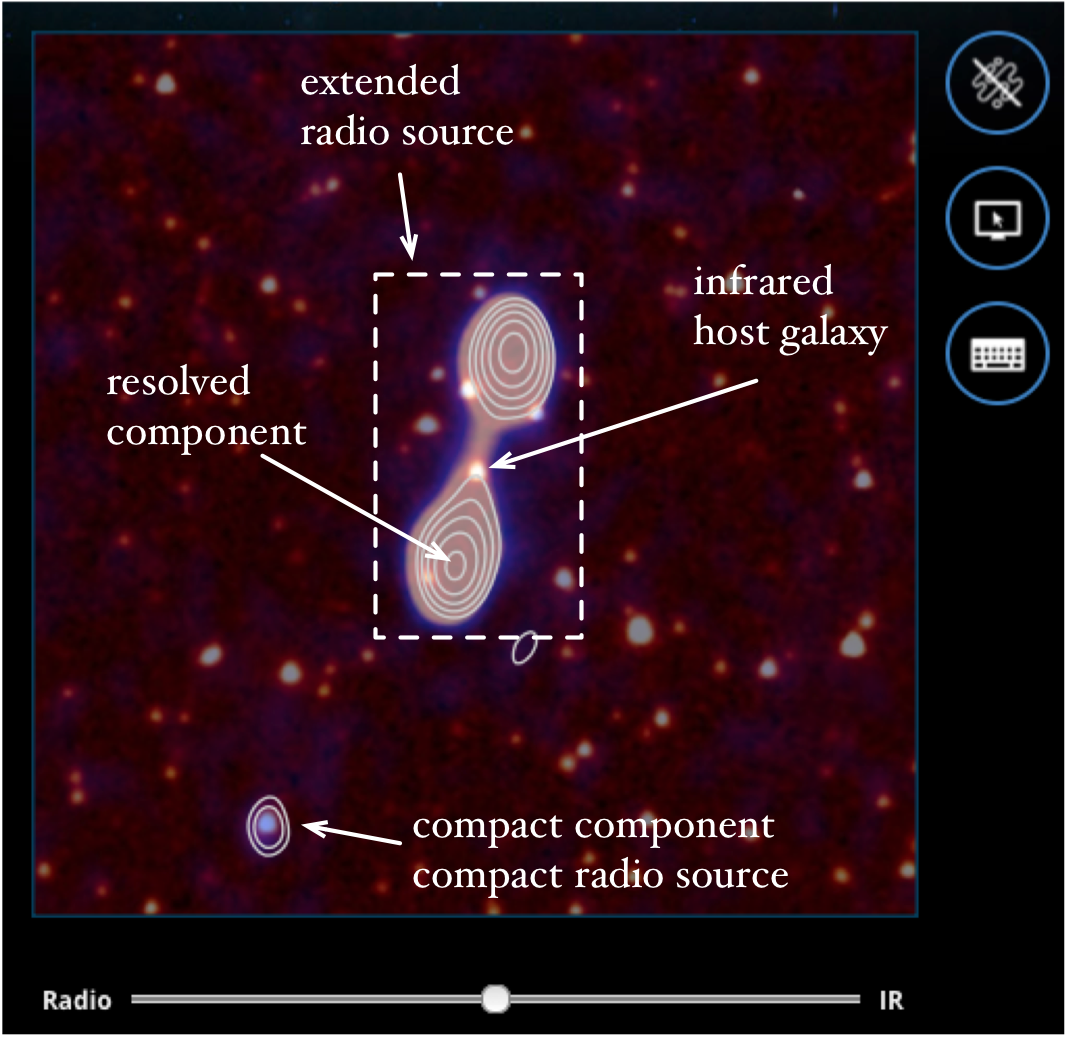
\includegraphics[width=0.75\linewidth]{images/fig1.png}
    \caption{The Radio Galaxy Zoo tutorial image illustrating key definitions
      used throughout this paper. A colour version of this figure is available
      online.}\label{fig1}
  \end{center}
  \end{figure}

\section{Data}\label{sec:data}

  We use data from the citizen science project Radio Galaxy Zoo
  \citep{banfield15}, the Australia Telescope Large Area Survey
  \citep[ATLAS;][]{norris06,franzen15}, and the \emph{Spitzer} Wide-area Infrared
  Extragalactic survey \citep[SWIRE;][]{lonsdale03swire, surace05swire}. Radio Galaxy Zoo also includes data from the Faint Images of the
    Radio Sky at Twenty-Centimeters \citep[FIRST;][]{white97first}. However, here we focus only on Radio Galaxy Zoo data from ATLAS and SWIRE.

  \subsection{ATLAS}\label{sec:atlas}
    \begin{table}
      \caption{Catalogues of ATLAS/SWIRE cross-identifications for the CDFS
        and ELAIS-S1 fields. The method used to generate each catalogue is
        shown, along with the number of radio components cross-identified in each
        field.}
      \label{tab:atlas-cids}
      \begin{tabular}{llcc}
        \hline
        Catalogue & Method & CDFS & ELAIS-S1\\
        \hline
        \citet{norris06} & Manual & 784 & 0\\
        \citet{middelberg08} & Manual & 0 & 1366\\
        \citet{fan15} & Bayesian models & 784 & 0\\
        Weston et al. (in prep) & Likelihood ratio & 3078 & 2113\\
        Wong et al. (in prep) & Crowdsourcing & 2460 & 0 \\
        \hline
      \end{tabular}
    \end{table}

    ATLAS is a pilot survey for the EMU \citep{norris11} survey, which will
    cover the entire southern sky south of $+30$ deg and is expected to
    detect approximately 70 million new radio sources. EMU will be conducted
    at the same depth and resolution as ATLAS, so methods developed for
    processing ATLAS data are expected to work for EMU. ATLAS is a wide-area
    radio survey of the CDFS and ELAIS-S1 fields at 1.4~GHz with a sensitivity
    of 14 and \unit{17}{\micro\jansky} on CDFS and ELAIS-S1 respectively. CDFS
    covers 3.6~deg$^2$ and contains 3034 radio components above a signal-to-noise ratio of 5.
    ELAIS-S1 covers 2.7~deg$^2$ and contains 2084 radio components above a signal-to-noise ratio of 5 \citep{franzen15}. \autoref{tab:atlas-cids} summarises
    catalogues that cross-identify radio components in ATLAS with host
    galaxies in SWIRE. In our work, we train our methods on CDFS and test these methods on both CDFS and ELAIS-S1.  This ensures our methods are transferable to different areas of the sky observed by the same telescope as will be the case for EMU.

  \subsection{SWIRE}\label{sec:swire}

    SWIRE \citep{lonsdale03swire, surace05swire} is a wide-area infrared
    survey at the four IRAC wavelengths 3.6, 4.5, 5.8, and
    \unit{8.0}{\micro\meter} \citep{lonsdale03swire}. It covers eight fields, including CDFS and ELAIS-S1. SWIRE is the source of infrared
    observations for cross-identification with ATLAS. SWIRE catalogues 221~535
    infrared objects in CDFS and 186~059 infrared objects in ELAIS-S1 above a signal-to-noise ratio of 5.

  \subsection{Radio Galaxy Zoo}\label{sec:rgz}

    Radio Galaxy Zoo asks volunteers to cross-identify radio components with
    their infrared host galaxies. There are a total of 2460 radio
    components in Radio Galaxy Zoo sourced from ATLAS. These
    components are cross-identified by Radio Galaxy Zoo participants to host galaxies detected in SWIRE.
    A more detailed description can be found in
    \citet{banfield15} and a full description of how the Radio Galaxy Zoo Data Release 1 catalogue used in this work\footnote{The Radio Galaxy Zoo Data Release 1 catalogue will only
    include cross-identifications for which over 65 per cent of volunteers
    agree. However, we use data from all volunteers.}
    is generated can be found in Wong et al. (in prep).

     The ATLAS~CDFS radio components that appear in Radio Galaxy Zoo are both unresolved and resolved radio components from the third data release of ATLAS by \citet{franzen15}.  Each radio component was fit with a two-dimensional
    Gaussian. Depending on the residual of the fit, more than one Gaussian may
    be fit to one region of radio emission.  Each of these Gaussian fits is
    listed as a radio component in the ATLAS catalogue. The brightest radio
    component from the multiple Gaussian fit is called the `primary
    component'. Each primary component found in the ATLAS DR3 component
    catalogue appears in Radio Galaxy Zoo. Non-primary components may appear
    within the image of a primary component, but do not have their own entry
    in Radio Galaxy Zoo. We will henceforth only discuss the primary
    components.

  \section{Method}\label{sec:method}
    \begin{figure}
      \centering
      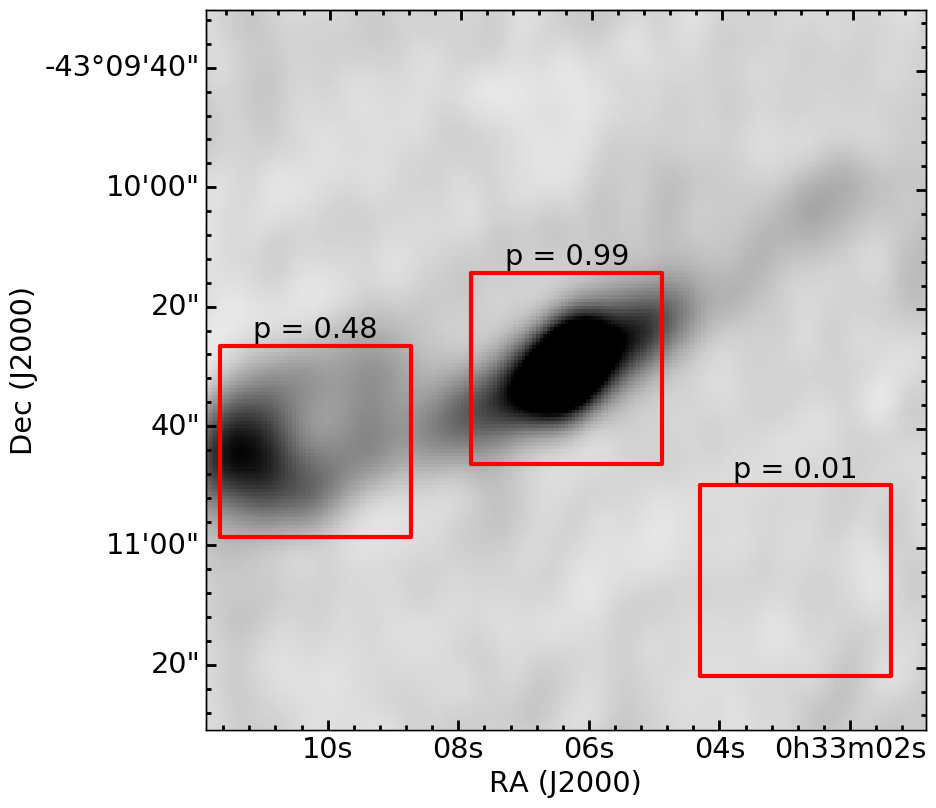
\includegraphics[width=\columnwidth]{images/fig2-jkb.png}
      \caption{An example of localising the host galaxy of a radio source using
        our method. This image is a radio image from ATLAS and is centred on
        $\alpha = 00^\text{h}33^\text{m}06.36^\text{s}, \delta =
        -43^\circ{}10'30.1''$. Boxes represent $32 \times 32$ pixel windows
        centred on various locations in the image. The image contained in each
        window is used to represent the location that the window is centred
        on. The probabilities of each patch coinciding with the host galaxy
        would then be estimated by a classification model. The probabilities
        shown are for illustration only. In this example, the centre window of
        the image would be chosen as the location of the host galaxy, as the
        window centred on it has the highest probability.}
      \label{fig:windows}
    \end{figure}

  \subsection{Cross-identification as binary
  classification}\label{cross-identification-as-binary-classification}
    \begin{figure}
      \centering
      % http://www.texample.net/tikz/examples/simple-flow-chart/
      \tikzstyle{decision} = [diamond, draw, fill=white,
          text width=4.5em, text badly centered, inner sep=0pt]
      \tikzstyle{block} = [rectangle, draw, fill=white,
          text width=5em, text centered, rounded corners, minimum height=4em]
      \tikzstyle{line} = [draw, -latex']
      \begin{tikzpicture}[node distance=6mm, auto]
        \node [block] (init) {input radio source};
        \node [decision, right= of init] (iscompact) {compact?};
        \node [block, below= of iscompact] (compact) {find nearest infrared object};
        \node [block, right= of iscompact] (resolved) {find nearby infrared objects};
        \node [block, fill=black!10, right= of resolved] (classify) {classify objects};
        \node [block, below= of classify] (best) {choose object based on probability};
        \coordinate (middle) at ($(compact)!0.5!(best)$);
        \node [block, below= of middle, fill=green!10] (done) {\textbf{host galaxy}};
        \path [line] (init) -- (iscompact);
        \path [line] (iscompact) -- (compact) node [midway] {yes};
        \path [line] (compact) -- (done);
        \path [line] (iscompact) -- (resolved) node [midway] {no};
        \path [line] (resolved) -- (classify);
        \path [line] (classify) -- (best);
        \path [line] (best) -- (done);
      \end{tikzpicture}
      \caption{A cross-identification method employing a binary classifier. As
        input we accept a radio source. If the source is compact, we select
        the nearest infrared object as the host galaxy. If the source is
        resolved, we classify all infrared objects nearby within radius $R$
        and select the highest probability object as the host galaxy. The grey
        box is the classifier, which can be any binary classifier that outputs
        a probability.}
      \label{fig:flowchart}
    \end{figure}

    We focus on the problem of host galaxy cross-identification without using
    radio morphology information. Given a radio component, we want to find the
    corresponding host galaxy as a human would. The input is a $2' \times 2'$
    radio image and a corresponding infrared image to match the size of the
    images used by Radio Galaxy Zoo. We make the assumption that each radio
    image represents a single, complex extended source. This limitation is
    discussed in \autoref{sec:limitations}. The radio cross-identification
    task is then formalised as the computer vision problem of object localisation: given a radio
    image and an infrared image centred on a radio component, locate the host
    galaxy of the source containing the radio component.

    A common approach to object localisation is to estimate the probability
    that each location in an image is coincident with the desired object,
    called a sliding window method \citep[e.g.][]{rowley1996facedetection}.
    Fixed-size windows of the image are taken centred on each pixel and we
    estimate the probability that the pixel is the location of the object.
    This task can be made more efficient if we assume that the host galaxy is
    always detected in the infrared. We then only consider windows centred on
    infrared sources, which we call `candidate host galaxies'. This assumption
    usually holds in CDFS, except for a rare class of infrared-faint radio
    sources\footnote{\citet{norris06} found 22 such radio sources in their
    sample of 784 bright ATLAS components in CDFS.}. This defines a binary
    classification task where given a candidate host galaxy we compute the
    probability that it is a host galaxy. We refer to this binary
    classification task as the `galaxy classification task' (GCT). To find the host
    galaxy given a radio source, we can classify each galaxy within 1~arcmin
    of the source and select the host galaxy based on the probability output
    by a classifier. We refer to this as the `cross-identification task' (X-ID). Our
    approach is illustrated in \autoref{fig:windows}.

    Solving the galaxy classification task amounts to modelling a function $f$
    from infrared sources $\mathcal{X}$ to the probability that an infrared
    source belongs to a binary class in $\mathcal{Y} = \{0, 1\}$:
    \begin{equation}
        f(x) \coloneqq \text{Pr}\left(\mathcal{Y} = 1 \mid \mathcal X = x\right)\,\,\,\,.
    \end{equation}
    The space of infrared sources $\mathcal{X}$ needs to be encoded as a vector
    for the models we will use. We describe this in
    \autoref{vector-representation-of-infrared-sources}. There are many options
    for modelling $f$. In this paper we apply three different models: logistic
    regression, random forests, and convolutional neural networks.

    Going from the galaxy classification task to the cross-identification task
    requires choosing the host galaxy based on the probability that each
    galaxy is a host galaxy. One approach would be to select the galaxy with
    the highest estimated class probability, i.e. the host galaxy is the candidate galaxy $x$ that maximises $f(x)$. This fails if there are multiple host galaxies within the $2' \times
    2'$ image, as only one host galaxy can be the maximum. An example of such
    an image is shown in \autoref{fig:broken-isolation}. Instead, we weight
    the estimated class probability of each candidate host galaxy by a Gaussian function of
    its angular separation from the radio component we want to cross-identify,
    and then select the maximum weighted probability.
    The Gaussian introduces dependence on the radio component we want to cross-identify and hence allows cross-identification of multiple host galaxies in the same image. It also acts as a prior for the host galaxy location. The standard deviation of the
    Gaussian, $\sigma$, controls the influence of the Gaussian on the final
    cross-identification. In the limit where $\sigma \to 0$, our approach is
    equivalent to a nearest-neighbours approach where we select the nearest
    infrared object to the radio component as the host galaxy. In the limit
    where $\sigma \to \infty$, we maximise the probability output by the
    classifier as above. We take $\sigma = 30''$ as this was the best value found by a grid search.

    We can improve upon this method by filtering out compact radio sources,
    which are much easier to cross-identify --- the nearest SWIRE object may
    be identified as the host galaxy, or a more complex method such as
    likelihood ratios may be applied (see Weston et al. in prep). A full
    cross-identification pipeline making use of this alongside a binary
    classifier is shown in \autoref{fig:flowchart}.

  \subsection{Limitations of our approach}
    \label{sec:limitations}

     \begin{figure}
      \centering
      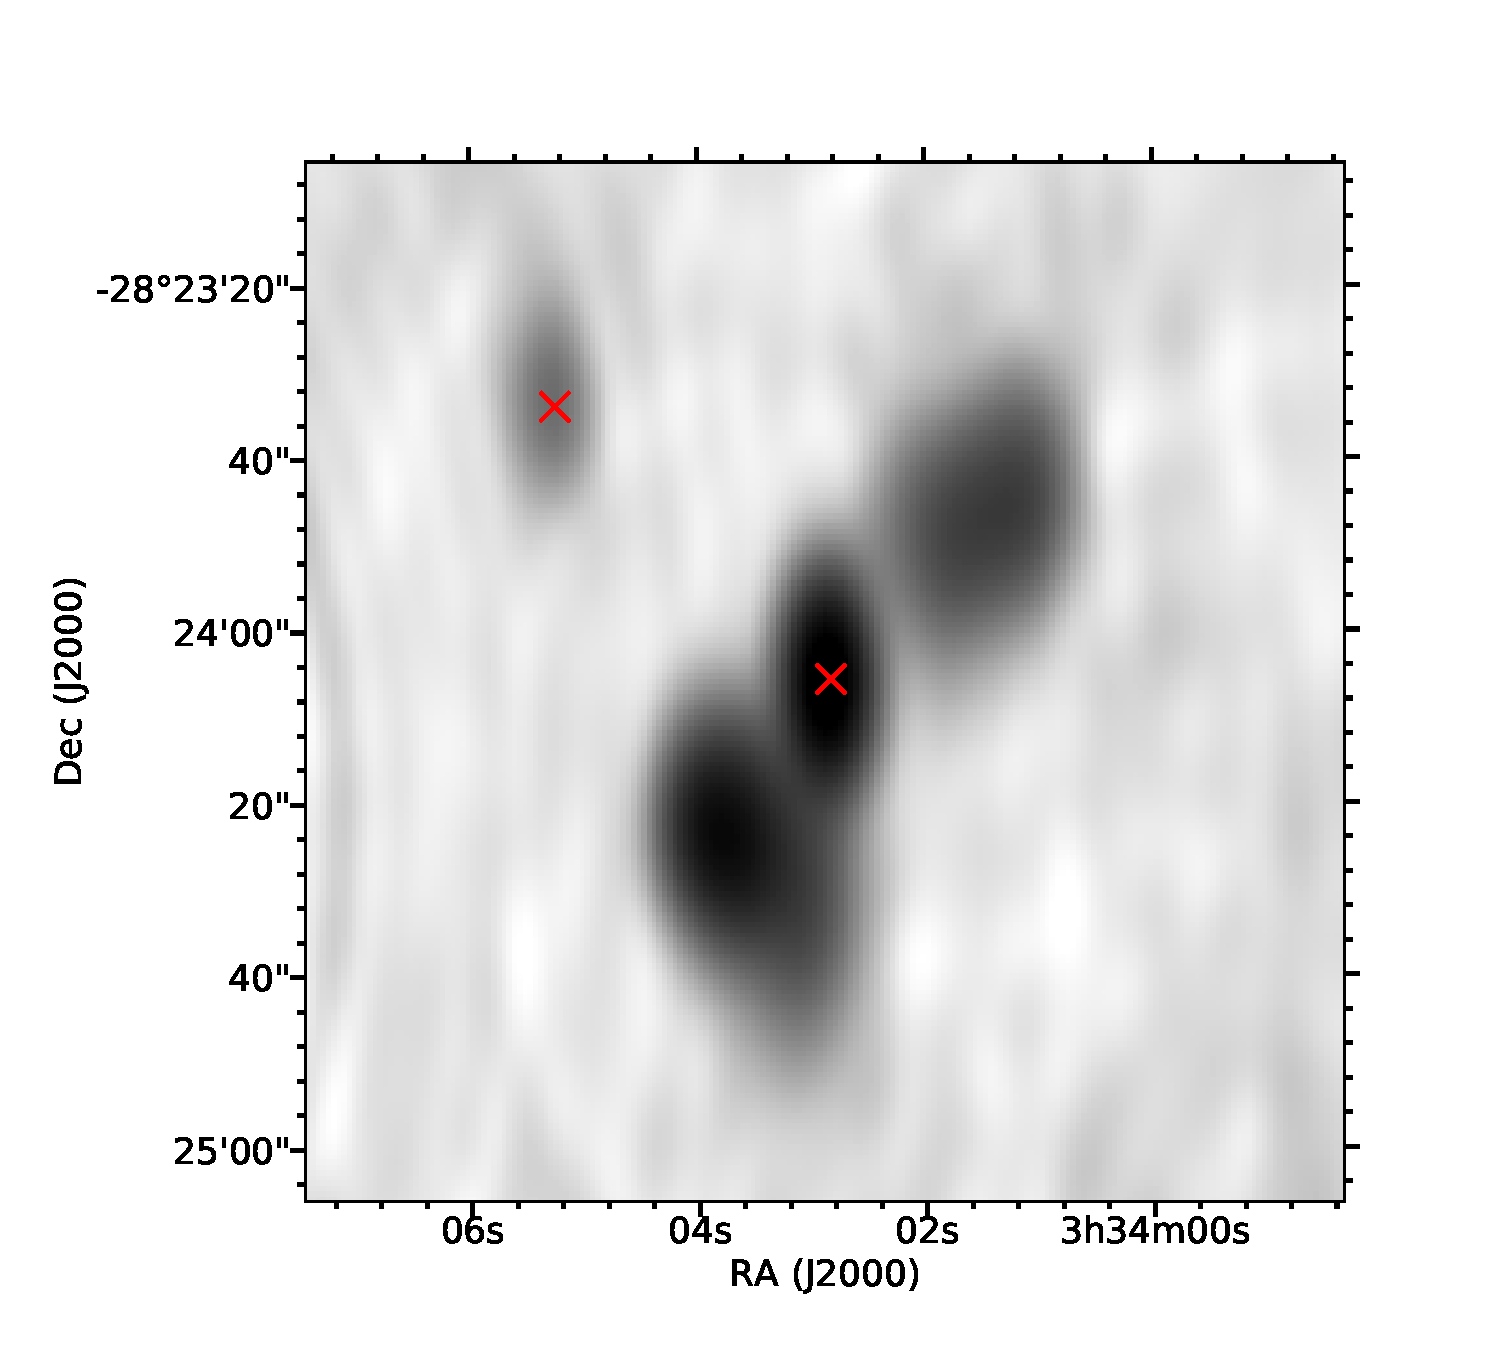
\includegraphics[width=\linewidth]{images/CI0077C1_fig.pdf}
      \caption{$2'$-wide radio image centred on ATLAS3\textunderscore{}J033402.87-282405.8C.
        %(ARG0003r2v)
        This radio source breaks the assumption that there are no other radio
        sources within 1~arcmin of the source. Another radio source is visible
        to the upper-left. Host galaxies found by Radio Galaxy Zoo volunteers
        are shown by a cross.}
      \label{fig:broken-isolation}
    \end{figure}

      \begin{figure}
      \centering
      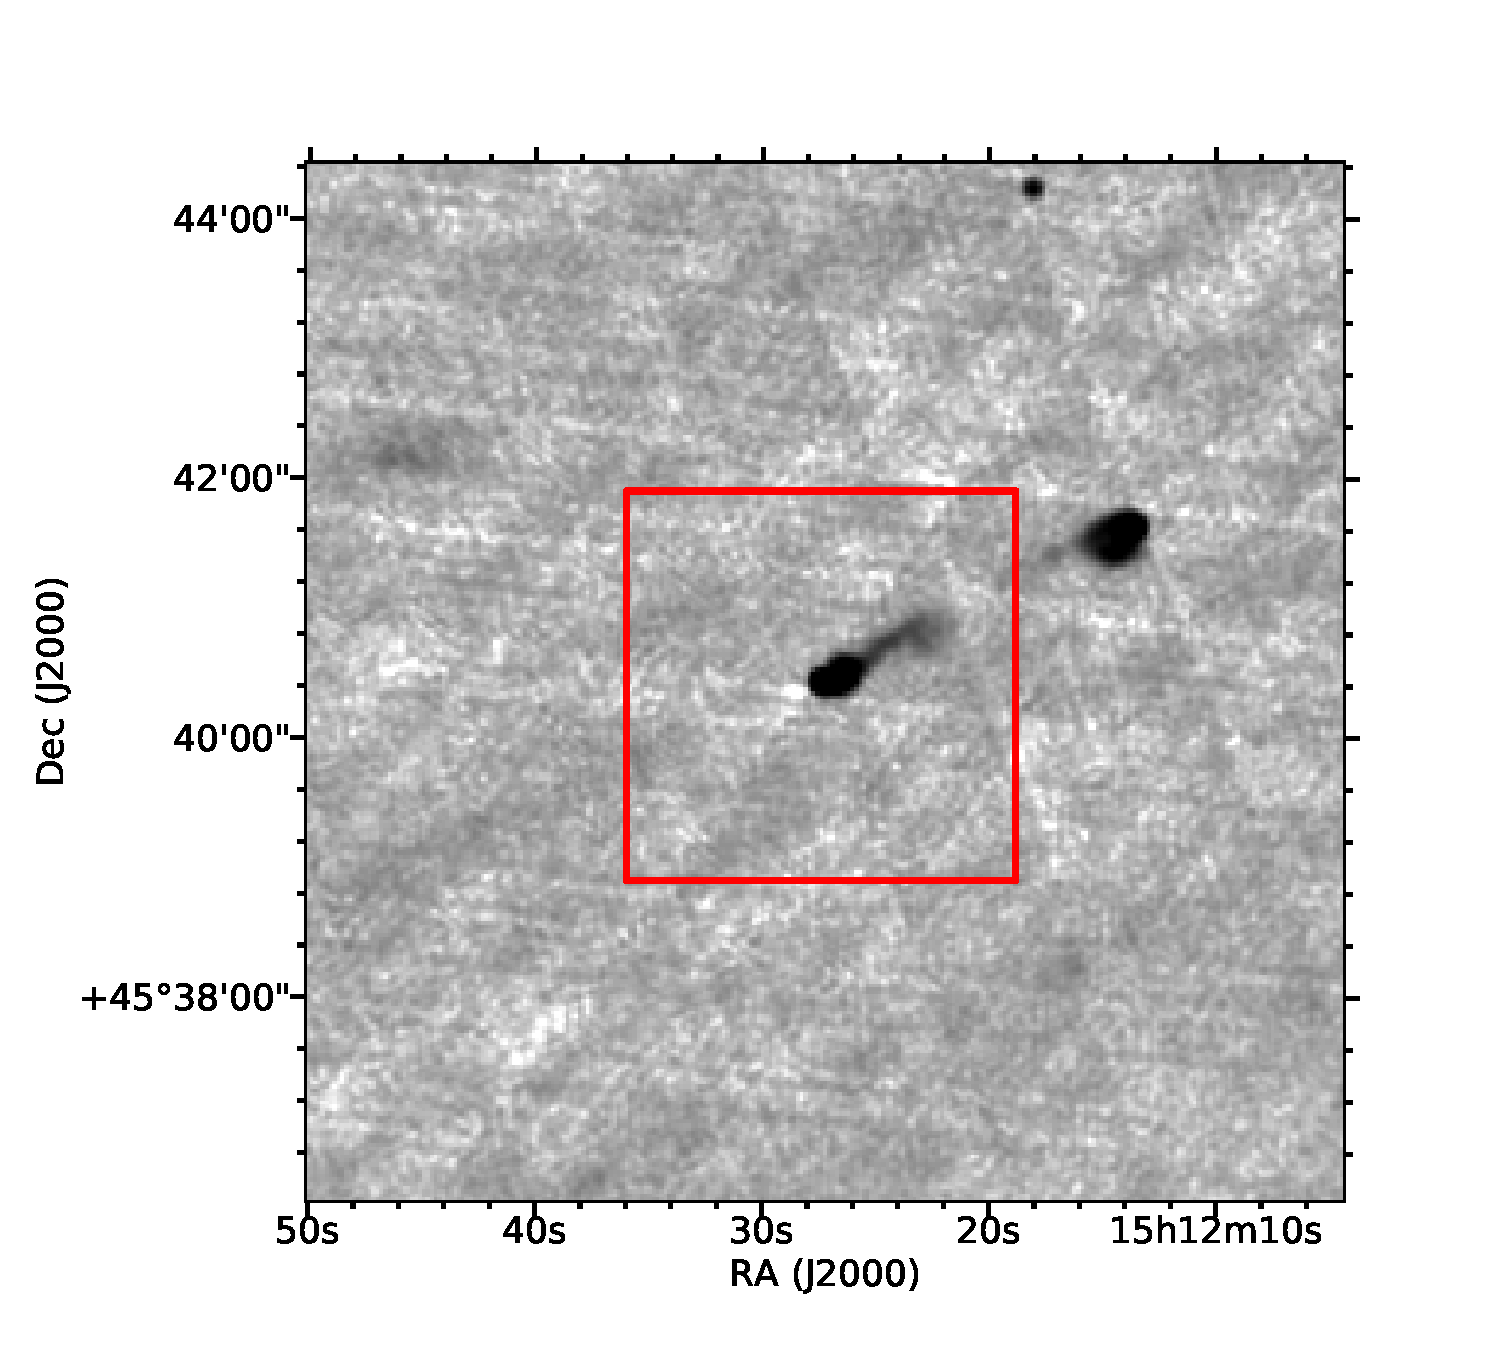
\includegraphics[width=\linewidth]{images/FIRSTJ151227_fig.pdf}
      \caption{A $8'$-wide radio image from FIRST, centred on
        FIRSTJ151227.2+454026. The $3'$-wide red box indicates the boundaries of
        the image of this radio component shown to volunteers in Radio Galaxy
        Zoo. This radio source breaks our assumption that the whole radio source
        is visible in the chosen radius. As one of the lobes of the radio source
        is outside of the image, a volunteer (or automated algorithm) looking at
        the $3'$-wide image may be unable to determine that this is a radio
        double or locate the host galaxy.}
      \label{fig:broken-contains}
    \end{figure}
        \begin{figure}
      \centering
      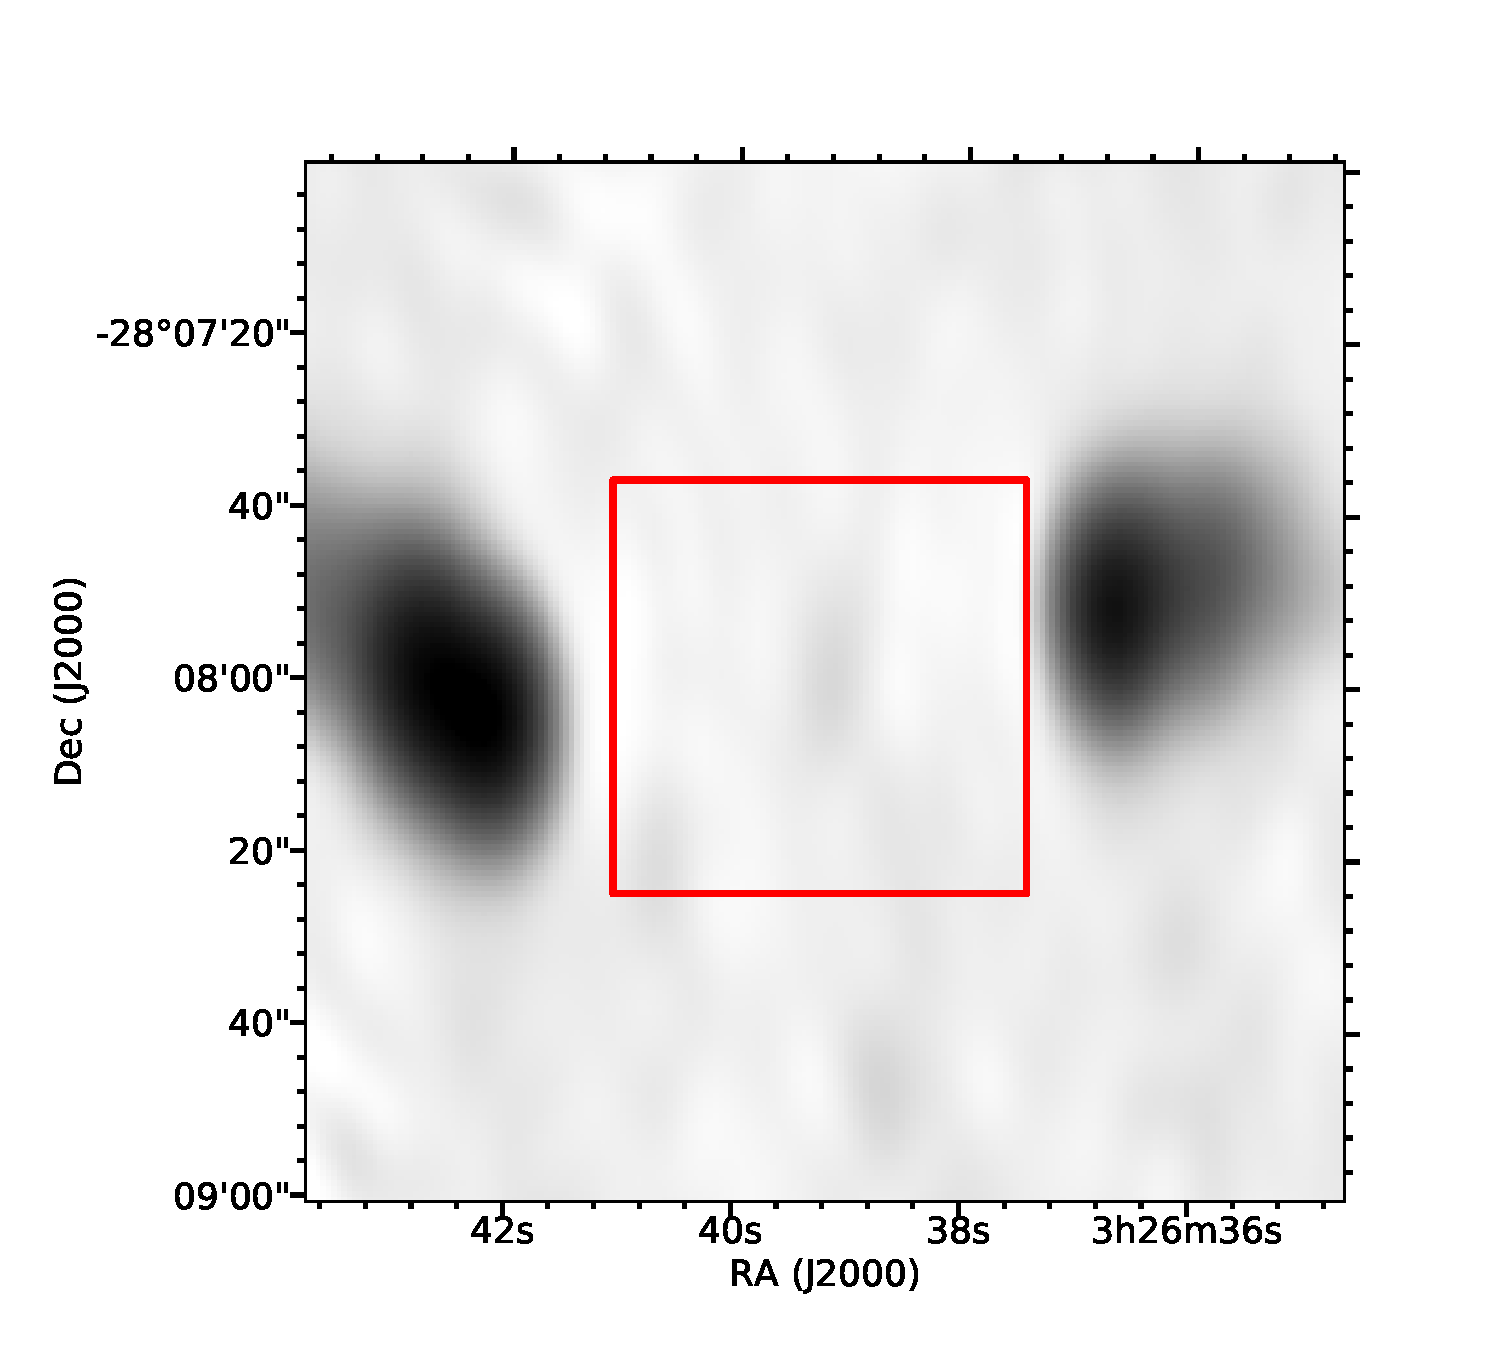
\includegraphics[width=\linewidth]{images/CI2363_fig.pdf}
      \caption{A radio image centred on $\alpha =
        03^\text{h}26^\text{m}39.12^\text{s}$, $\delta = -28^\circ{}07'58.80''$.        %ARG0003sky
        This is an example of a radio source where the window centred on the
        host galaxy, shown as a rectangle, does not contain enough radio
        information to correctly identify the galaxy as the host.}
      \label{fig:broken-window-size}
    \end{figure}

    We make a number of assumptions to relate the cross-identification task to
    the galaxy classification task:
    \begin{itemize}
      \item A radio image represents a whole, single radio source.
      \item The host galaxy of a radio component is within 1~arcmin of the
        component.
      \item The host galaxy of a radio component is closer on the sky to the
        radio component than any other host galaxy.
      \item The host galaxy appears in the SWIRE catalogue.
    \end{itemize}
    These assumptions limit the effectiveness of our approach, regardless of
    how accurate our binary classification may be.

    The main limitation is in choosing the image width and candidate search
    radius. If the radio image does not contain the whole source, then we are
    missing radio information useful for finding the host galaxy. If the radio
    image contains multiple sources, then we may be giving our classifiers
    irrelevant information. If the search radius is too small, we may not
    consider the host galaxy as a candidate. If the search radius is too
    large, we may consider multiple host galaxies (though this is somewhat
    mediated by the Gaussian multiplier). These kinds of size problems are
    difficult even for non-automated methods as radio sources can be extremely
    wide --- for example, Radio Galaxy Zoo found a radio giant that spanned
    over three different images presented to volunteers and the full source
    was only cross-identified by the efforts of citizen scientists
    \citep{banfield15}. An example of a radio image where part of the radio
    source is outside the search radius is shown in
    \autoref{fig:broken-contains}.

    A related issue is that we need to choose a window size for the image
    representations of each SWIRE object. If this image is too small, radio
    emission may extend past the edges of the window, and it may be impossible
    to identify the galaxy as a host galaxy. If the image is too large, then
    too much information will be included and it will be difficult or
    computationally expensive to classify. We chose a window size of $32
    \times 32$ pixels, corresponding to approximately $18'' \times 18''$ in
    CDFS. This is shown as red rectangles in \autoref{fig:windows} and
    \autoref{fig:broken-window-size}.

    The assumption that the host galaxy of a radio component is closer on the
    sky to the radio component than any other host galaxy is required for the
    Gaussian multiplier to correctly break ties.

    We only need the assumption that the host galaxy appears in SWIRE to
    incorporate galaxy-specific features
    (\autoref{vector-representation-of-infrared-sources}) and to improve
    efficiency. Our method is applicable even to infrared-faint radio sources
    by considering every pixel as a candidate location as would be done in the
    original computer vision approach.

    Our assumptions impose an upper bound on how well we can cross-identify
    radio sources. We estimate this upper bound in \autoref{sec:relation}.

  \subsection{Feature vector representation of infrared sources}
  \label{vector-representation-of-infrared-sources}

    Classification methods require that the inputs to be classified are
    represented by an array of real values called feature vectors. We thus
    need to choose a feature vector representation of our candidate host
    galaxies.

    We use the SWIRE catalogue to find candidate
    hosts to classify. Candidates are represented by a a 32 $\times$ 32 pixel radio image from
    ATLAS, centered on the location of the candidate.
    As the visual appearance of infrared objects is likely irrelevant to
    whether the galaxy is a host galaxy, the candidate host location encodes
    almost all information we could gain from the infrared image. We therefore
    do not use the infrared image for object localisation in this work.

    We represent each candidate host as 1034 real-valued features. For a given
    candidate host, these features are:
    \begin{itemize}
      \item the 6 logarithms of the ratios of fluxes of the candidate
        host in the four IRAC wavelengths;
      \item the stellarity index of the host in both 3.6 and
        \unit{4.5}{\micro\meter};
      \item the flux of the host in \unit{3.6}{\micro\meter};
      \item the radial distance between the candidate host and the nearest
        radio component in the ATLAS catalogue; and
      \item a 32 $\times$ 32 pixel image from ATLAS (approximately $18''
        \times 18''$), centred on the candidate host.
    \end{itemize}

    The infrared fluxes provide insight into the properties of the host galaxy
    of the radio emission. The 3.6 and \unit{4.5}{\micro\meter} fluxes trace
    both galaxies with faint polycyclic aromatic hydrocarbon (PAH) emission and
    elliptical galaxies dominated by old stellar popluations. The
    \unit{5.8}{\micro\meter} flux selects galaxies where the infrared emission
    is dominated by non-equilibrium emission of dust grains (PAH destruction
    by the hard UV spectrum of AGN), while the \unit{8.0}{\micro\meter} flux
    traces strong PAH emission at low redshift \citep{Sajina2005}.
    The stellarity index represents how likely the object is to be a star
    rather than a galaxy.

    We use the pixels of each $32 \times 32$ radio image as independent
    features for all classifiers, with the convolutional neural network
    automatically extracting
    features that are relevant. Other features of the radio components may be used instead of the pixel values, but there has been limited research on extracting
    such features. \citet{proctor06} describes hand-selected
    features for radio doubles in FIRST, and \citet{aniyan17cnn} and
    Lukic et al. (in prep) make use of deep convolutional neural networks
    which automatically extract features as part of classification. A more
    comprehensive investigation of features is beyond the scope of this initial study, and is a good
    avenue for potential improvement in our pipeline.

  \subsection{Classifiers}\label{sec:classifiers}

    We use three different classifiers as our binary classification model:
    logistic regression, convolutional neural networks, and random forests.
    These classifiers cover three different approaches to machine learning.
    Logistic regression is a probabilistic binary classification model.
    It is linear in the
    feature space and outputs the probability that the input has a positive
    label~\citep[Chap. 4]{bishop06ml}.
    Convolutional neural networks (CNN) are a biologically-inspired
    prediction model for prediction with image inputs.
    They have recently produced good results on large image-based datasets
    in astronomy \citep[e.g.][Lukic et al. in prep]{dieleman15cnn}.
    Random forests are an ensemble of decision
    trees~\citep{breiman01random-forest}. It considers multiple subsamples
    of the training set, where each bootstrap subsample is sampled with
    replacement from the training set. To classify a new data
    point, the random forest takes the weighted average of all
    classifications produced by each decision tree.

    Further details and background of these models are available in the
    supplement\footnote{\url{https://radiogalaxyzoo.github.io/atlas-xid/}}.

  \subsection{Labels}\label{sec:labels}
    \begin{figure}
      \centering
      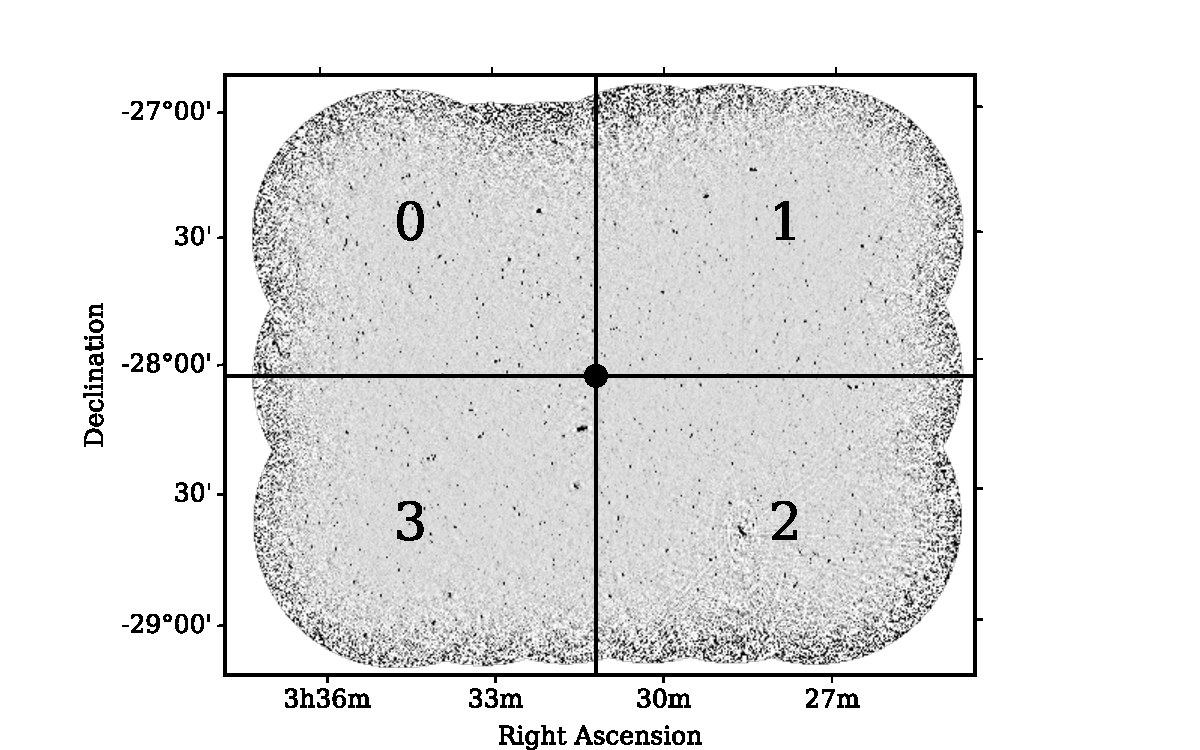
\includegraphics[width=\columnwidth]{images/quadrants.pdf}
      \caption{CDFS field training and testing quadrants labelled 0 -- 3. The
        central dot is located at $\alpha = 03^\text{h}31^\text{m}12^\text{s},
        \delta = -28^\circ{}06'00''$. The quadrants were chosen such that
        there are similar numbers of radio sources in each
        quadrant.\label{fig:quadrants}}
    \end{figure}

    \begin{table}
      \caption{Number of compact and resolved radio objects in each CDFS quadrant. Radio Galaxy Zoo (RGZ) has more cross-identifications than the expert catalogue provides, and so has more objects in each quadrant for training.}
      \label{tab:radio-count}
      \begin{tabular}{lcccc}
        \hline
        Quadrant & Compact & Resolved & Compact & Resolved\\
        &&&(RGZ)&(RGZ)\\
        \hline
        0 & 126 & 24 & 410 & 43 \\
        1 & 99 & 21 & 659 & 54 \\
        2 & 61 & 24 & 555 & 57 \\
        3 & 95 & 18 & 631 & 51 \\
        \hline
        \textit{Total} & 381 & 87 & 2255 & 205\\
        \hline
      \end{tabular}
    \end{table}

    \begin{figure}
      \centering
      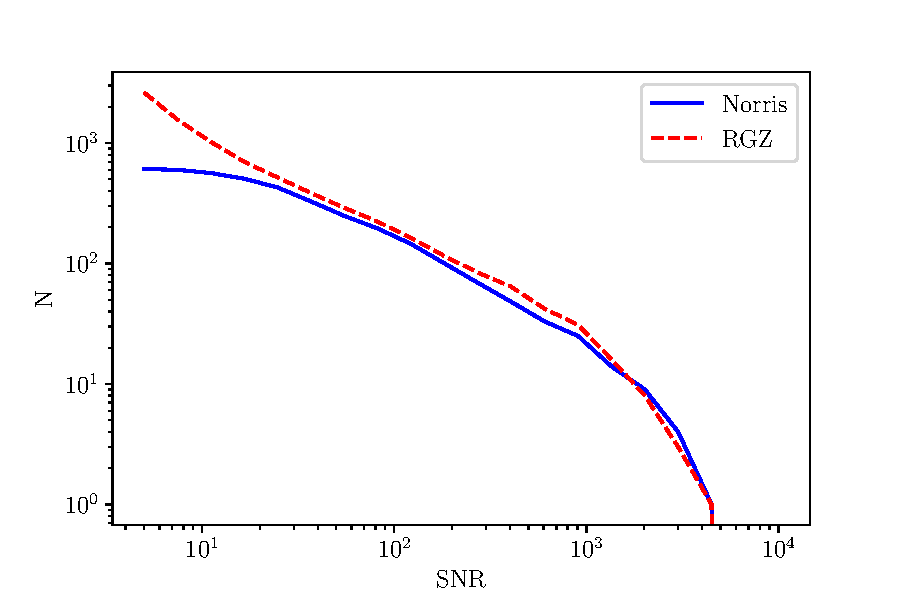
\includegraphics[width=\columnwidth]{images/snr_cutoff_cumulative.pdf}
      \caption{Number of radio components ($N$) in the expert (Norris) and Radio Galaxy
        Zoo (RGZ) training sets with different signal-to-noise (SNR) cutoffs.}
      \label{fig:distribution-cutoffs}
    \end{figure}

    Converting the Radio Galaxy Zoo and \citet{norris06} cross-identification
    catalogues to binary labels for infrared objects is a non-trivial task. One problem is that there is no clear way to capture radio morphology
    information in binary classification of infrared objects. Another problem is that there is no way to indicate
    \emph{which} radio object an infrared object is associated with, only that
    it is associated with \emph{some} radio object. We ignore these problems
    for this paper and make the na\"ive
    assumption that any given search radius contains only one host galaxy. This allows us to assume that if a candidate host galaxy in the search radius of a component is not the host galaxy of that component, then it is not a host galaxy at all.

    We then generate positive labels from a cross-identification catalogue.
    We decide that if an infrared object is listed in the catalogue, then it
    is assigned a positive label as a host galaxy. We then assign every other galaxy a negative label. This has some problems
    --- an example is that if the cross-identifier did not observe a radio
    object (e.g.~it was below the signal-to-noise ratio) then the host galaxy
    of that radio object would receive a negative label. This occurs with
    \citet{norris06} cross-identifications, as these are associated with the
    first data release of ATLAS. The first data release went to a 5$\sigma$
    flux density level of $S_{1.4} \geq 1 \text{ mJy beam}^{-1}$
    \citep{norris06}, compared to $S_{1.4} \geq \unit{85}{\micro\jansky}\text{
    beam}^{-1}$ for the third data release used by Radio Galaxy Zoo
    \citep{franzen15}. The labels from \citet{norris06} may therefore disagree with labels
    from Radio Galaxy Zoo even if they are both plausible. The difference in
    training set size at different flux cutoffs is shown in
    \autoref{fig:distribution-cutoffs}. We train and test our classifiers on
    infrared objects within a 1~arcmin radius of an ATLAS radio object.

  \subsection{Experimental Setup}
  \label{sec:experimental-setup}

    We trained binary classifiers on infrared objects in the CDFS field using two sets of labels. One label set was derived from
    Radio Galaxy Zoo cross-identifications and the other was derived from the
    \citet{norris06} cross-identification catalogue. We refer to these as the
    `Radio Galaxy Zoo labels' and the `expert labels' respectively. We divided the
    CDFS field into four quadrants for training and testing. The quadrants
    were centred on $\alpha = 52^\text{h}48^\text{m}00^\text{s},
    \delta = -28^\circ{}06'00''$ as shown in \autoref{fig:quadrants}. For
    each trial, one quadrant was used to draw test examples and the other three
    quadrants were used for training examples.

    We further divided the radio components into compact and resolved. Compact
    components are cross-identified by fitting a 2D Gaussian \citep[as
    in][]{norris06} and we would expect any machine learning approach for host
    cross-identification to attain high accuracy on this set. A radio component was
    considered resolved if
    \begin{equation}
        \ln \left(
          \frac{S_{\text{int}}}
               {S_{\text{peak}}}
        \right) > 2\sqrt{\left(
          \frac{\sigma_{S_{\text{int}}}}
               {S_{\text{int}}}
        \right)^2 + \left(
          \frac{\sigma_{S_{\text{peak}}}}
               {S_{\text{peak}}}
        \right)^2}\,\,\,\,,
    \end{equation}%
    where \(S_{\text{int}}\) is the integrated flux density and
    \(S_{\text{peak}}\) is the peak flux density
    \citep[following][]{franzen15}.

    Candidate hosts were selected from the SWIRE catalogue. For a given subset
    of radio components, all SWIRE objects within 1~arcmin of all radio
    components in the subset were added to the associated SWIRE subset. In the
    context of the galaxy classification task, we refer to SWIRE objects
    within 1~arcmin of a compact radio component as part of the `compact set',
    and SWIRE objects within 1~arcmin of a resolved radio component as part of
    the `resolved set'.

    To reduce
    bias in the testing data due to the expert labels being generated from a
    shallower data release of ATLAS, a SWIRE object was only included in the test
    set if it was within 1~arcmin of a radio object with a cross-identification
    in both the \citet{norris06} catalogue and the Radio Galaxy Zoo catalogue.

    Each classifier was trained on the training examples and used to predict
    labels for the test examples. The predicted labels were compared to the
    expert labels and the balanced accuracy was computed. Balanced accuracy is the average of the accuracy on the positive class and the accuracy on the negative class, and is not sensitive to class imbalance. The galaxy classification task has highly imbalanced classes --- in
    our total set of SWIRE objects within 1~arcmin of an ATLAS object, only
    4~per cent have positive labels.
    Only examples within 1~arcmin of ATLAS
    objects in the first ATLAS data release \citep{norris06} were used to
    compute accuracy, as these were the only ATLAS objects with expert labels.

    We then used the estimated class probabilities to predict the host galaxy for
    each radio component cross-identified by both \citet{norris06} and Radio
    Galaxy Zoo. For each SWIRE object within 1~arcmin of the radio component,
    the probability of the object having a positive label was estimated using
    the trained binary classifiers. The SWIRE object with the highest Gaussian-weighted
    probability was chosen as the host galaxy. The accuracy for the cross-identification task was then estimated
    by counting how many predicted host galaxies matched the \citet{norris06}
    cross-identifications.

\section{Results}\label{sec:results}

  In this section we present accuracies of our method trained on CDFS and
  applied to CDFS and ELAIS-S1, as well as results motivating our accuracy
  measures and estimates of upper and lower
  bounds for cross-identification accuracy using our method.

  \subsection{Relation between binary classification and cross-identification}
  \label{sec:relation}

    \begin{figure}
      \centering
      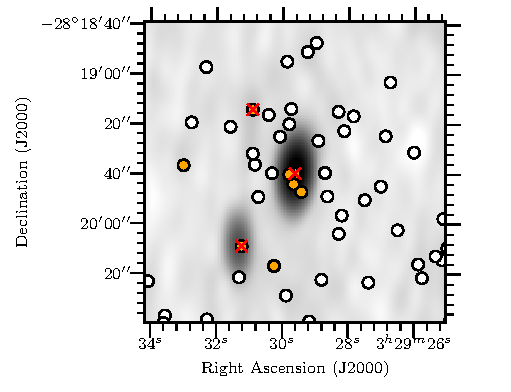
\includegraphics[width=\columnwidth]{images/positives.pdf}
      \caption{ATLAS3~J032929.61-281938.9. Radio Galaxy Zoo host galaxies are
      marked by crosses. SWIRE candidate host galaxies are circles, coloured orange
      circles have been assigned a `positive' label by a logistic regression
      classifier and white otherwise.
      \label{fig:positives}}
    \end{figure}

    \begin{figure}
      \centering
      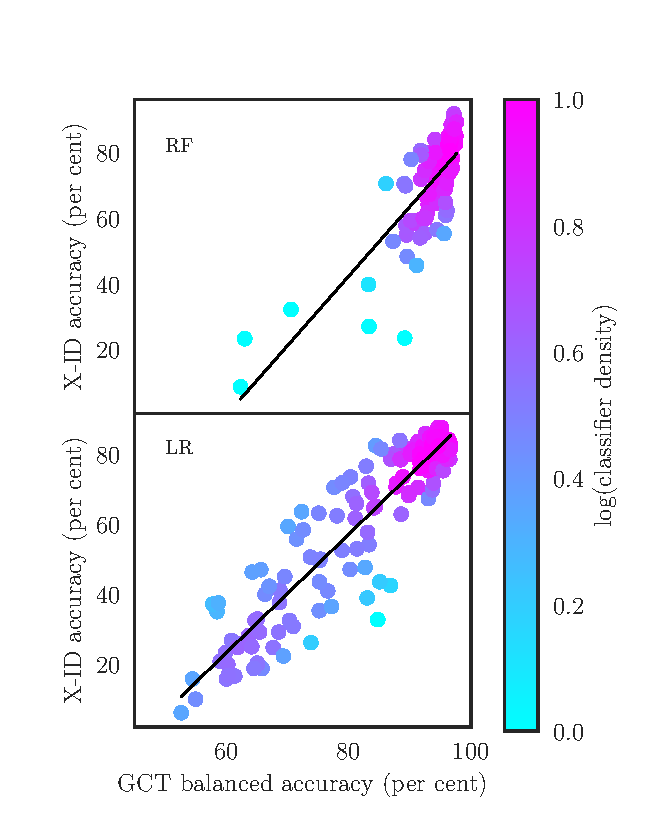
\includegraphics[width=\columnwidth]{images/gct-to-xid.pdf}
      \caption{Balanced accuracy on the galaxy classification task (GCT) plotted
      against accuracy on the cross-identification task (X-ID). RF indicates
      results from random forests, and LR indicates results from logistic
      regression. Classifiers were trained on random, small subsets of the
      training data to artificially restrict their accuracies. Colour shows
      the density of points on the plot estimated by a Gaussian kernel density
      estimate. The solid lines indicate the best linear fit; these fits have
      $R^2 = 0.92$ for logistic regression and $R^2 = 0.87$ for random
      forests. We did not include convolutional neural networks in this test,
      as training them is very computationally expensive. These results
      exclude classifiers witih balanced accuracies less than 51 per cent, as
      these are essentially random.
      \label{fig:gct-to-xid}}
    \end{figure}
  
    We can assess our classifiers either by their performance on the galaxy classification task or by their performance on the cross-identification task. Both performances are useful: performance on the galaxy classification task provides a robust and simple way to compare classifiers without the limitations of our specific formulation, and performance on the cross-identification task can be compared with other cross-identification methods. We therefore report two sets of accuracies: balanced accuracy for the galaxy classification task and accuracy for the cross-identification task. These accuracy measures are correlated and we show this correlation in \autoref{fig:gct-to-xid}. Fitting a line of best fit with \texttt{scipy} gives $R^2 = 0.92$ for logistic regression and $R^2 = 0.87$ for random forests.

    While performance on the galaxy classification task is correlated with performance on the cross-identification task, balanced accuracy does not completely capture the effectiveness of a binary classifier applied to the cross-identification task. This is because binary classifiers output a predicted label for each object in addition to the class probability, and it is this predicted label that is used to compute balanced accuracy. In the galaxy classification task, the classifier only needs to maximise the rate at which it correctly identifies host galaxies. This means there can be many `false positives' that do not affect cross-identification. An example of this is shown in \autoref{fig:positives}, where the classifier has identified 8 `host galaxies'. However, there are only three true host galaxies in this image --- one per radio component --- and so in the cross-identification task, only three of these galaxies will be identified as hosts.

    The formulation of cross-identification as binary classification also
    introduces limitations as described in \autoref{sec:limitations}, which
    impose upper limits on performance. Additionally, the classification
    pipeline described in \autoref{fig:flowchart} only uses the binary
    classification approach for non-compact objects, which imposes lower
    limits on performance. We estimate the upper limit on performance by
    assuming we have a `perfect' classifier which simply reads the correct
    label from the test set, and hence assign all true host galaxies a 100 per
    cent probability of being host galaxies. The accuracy of this
    classifier on the cross-identification task then represents the best
    possible cross-identification performance achievable under our
    assumptions. We estimate the lower limit on performance by taking a random
    classifier, which outputs random probabilities regardless of input galaxy.
    We expect any useful classifier to produce better results than this, so this
    represents the lowest expected cross-identification performance. We report
    the cross-identification accuracies of the perfect and random classifiers
    alongside the performance of other classifiers. We also report the accuracy of a nearest-neighbours approach, where the infrared object nearest to a radio component is chosen as its host galaxy. The upper estimates, lower estimates, and nearest-neighbour accuracy are shown as horizontal lines in \autoref{fig:cross-id-accuracy}
    for CDFS and \autoref{fig:elais-cross-id-accuracy} for ELAIS-S1.

  \subsection{Application to ATLAS~CDFS}

    \begin{figure}
    \centering
    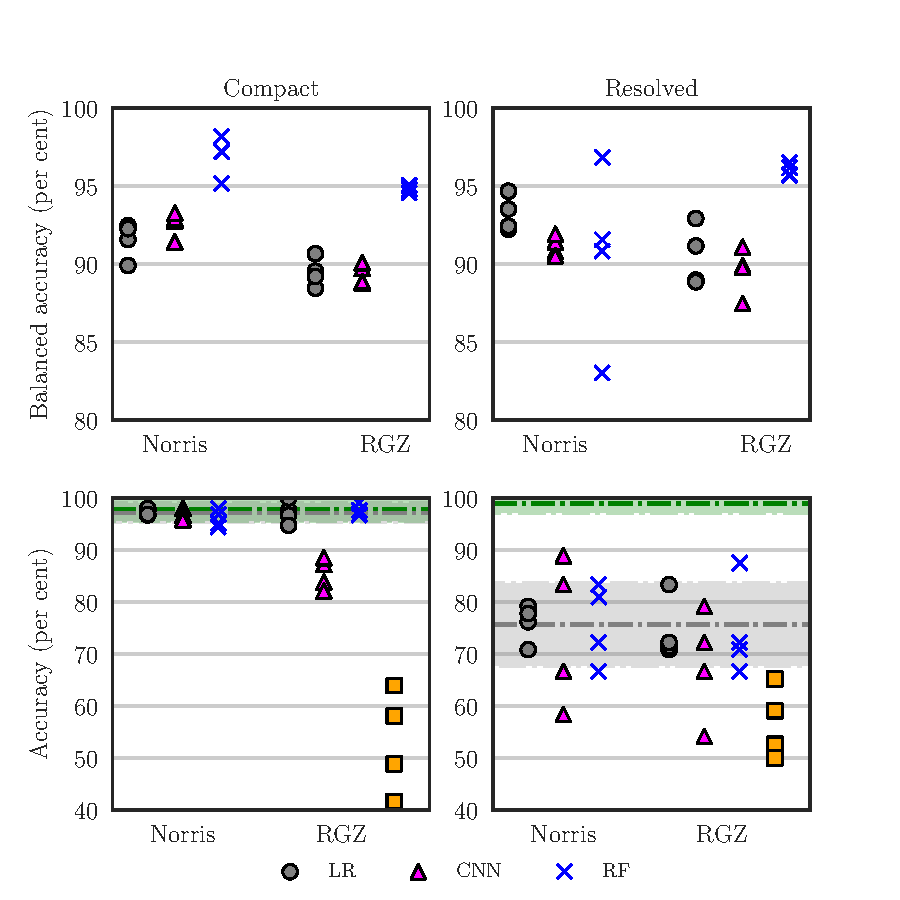
\includegraphics[width=\columnwidth]{images/cdfs-grid-new.pdf}
    \caption{Performance of logistic regression (LR), convolutional neural networks (CNN), and random forest (RF) classifiers. `Norris' indicates classifiers trained on the expert labels and `RGZ' indicates classifiers trained on the Radio Galaxy Zoo labels. The training and testing sets have been split into compact and resolved objects, with results on compact objects shown on the left and results on resolved objects shown on the right. Shown for comparison is the X-ID accuracy of the Radio Galaxy Zoo consensus cross-identifications (Labels). The X-ID accuracy attained by a perfect classifier is shown by a solid green line, and the X-ID accuracy of a nearest-neighbours approach is shown by a dashed grey line. The standard deviation of these accuracies across the four CDFS quadrants is shown by the shaded area. Note that the pipeline shown in \autoref{fig:flowchart} is not used for these results.
        \label{fig:ba}}
    \end{figure}

    \begin{figure}
      \centering
      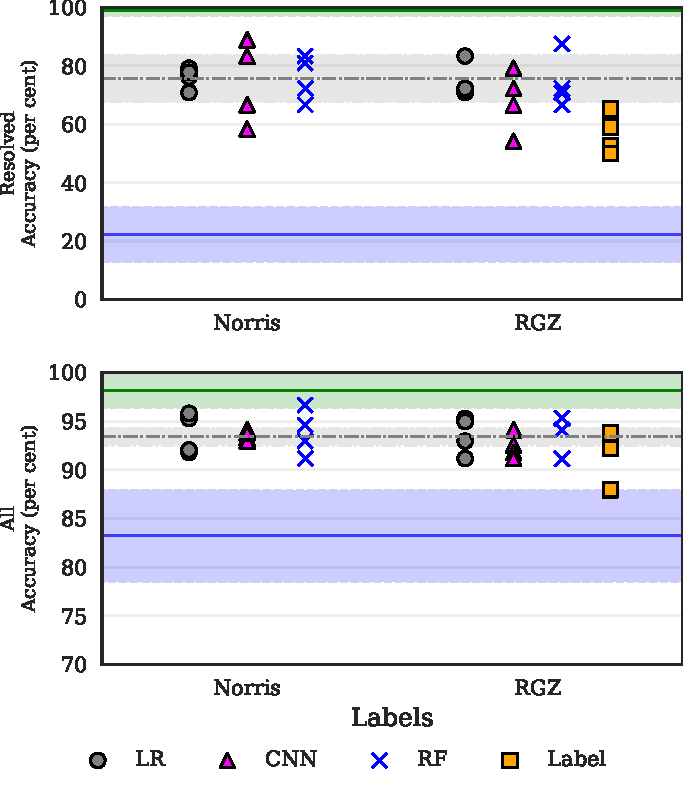
\includegraphics[width=0.9\columnwidth]{images/cdfs_cross_identification_grid.pdf}
      \caption{Performance of different classifiers on the cross-identification task. Markers and lines are as in \autoref{fig:ba}. The blue solid line indicates the performance of a random classifier and hence represents the minimum accuracy we expect to obtain. The standard deviation of this accuracy across 25 trials and 4 quadrants is shaded. The Radio Galaxy Zoo accuracies (`Labels') are below the axis and are marked by an arrow with the mean accuracy. Note that the pipeline shown in \autoref{fig:flowchart} is used here.
        \label{fig:cross-id-accuracy}}
    \end{figure}

    In \autoref{fig:ba} we plot the performance of logistic regression, random
    forests, and convolutional neural networks on both the galaxy
    classification task and the cross-identification task for resolved and
    compact sources. For comparison, we also plot the accuracy of Radio Galaxy
    Zoo and nearest neighbours on the cross-identifiction task. In \autoref{fig:cross-id-accuracy} we plot the performance of these classifiers on the full set of ATLAS~DR1 radio components using the pipeline in \autoref{fig:flowchart}.

    Differences between accuracies across training
    labels are well within error across the four quadrants, with convolutional neural networks on compact objects as the only exception. The spread of
    accuracies is similar for both sets of training labels, with the exception
    of random forests. The balanced accuracies of random forests trained on expert labels have a considerably higher spread than those trained on Radio Galaxy Zoo labels, likely because of the small size of the expert training set --- there are less than half the number of objects in the expert-labelled training set than the number of objects in the Radio Galaxy Zoo-labelled training set (\autoref{tab:radio-count}).

    Radio Galaxy Zoo-trained classifiers significantly outperform Radio Galaxy Zoo cross-identifications. Additionally, despite poor performance of Radio Galaxy Zoo on the cross-identification task, classifiers trained on these cross-identifications still perform comparably to those trained on expert labels. This shows the usefulness of crowdsourced training data, even when the data is noisy.

    Our classifiers perform comparably to a nearest-neighbours approach. For compact objects, this is to be expected --- indeed, nearest neighbours attains nearly 100 per cent accuracy on the compact test set. Our results do not improve on nearest neighbours for resolved objects. However, our method does allow for improvement on nearest neighbours with a sufficiently good binary classifier: a `perfect' classifier attains nearly 100 per cent accuracy on resolved sources. This shows that our method may be useful provided that a good binary classifier can be trained. The most obvious place for improvement is in feature selection; we use pixels of radio images directly and these are likely not conducive to good performance on the galaxy classification task. Convolutional neural networks, which are able to extract features from images, \emph{should} work better, but these require far more training data than the other methods we have applied and the small size of ATLAS thus results in poor performance.

    We noted in \autoref{sec:labels} that the test set of expert labels, derived from the initial ATLAS data release, was less deep than the third data release used by Radio Galaxy Zoo and this paper, introducing a source of label noise in the testing labels. Specifically, true host galaxies may be misidentified as non-host galaxies if the associated radio source was below the 5 signal-to-noise limit in ATLAS DR1 but not in ATLAS DR3. This has the effect of reducing the accuracy for Radio Galaxy Zoo-trained classifiers.

    We report the probabilities predicted by each classifier for each SWIRE
    object in the supplement. Probabilities reported for a given object
    were predicted by classifiers tested on the quadrant containing that
    object.

    For the cross-identification task, we report the accuracy of each
    classification model and training label set in
    \autoref{fig:cross-id-accuracy}. We report the averaged
    cross-identification accuracies across all four quadrants in the supplement.

    The predicted cross-identification for each ATLAS object is reported in
    the supplement. As with SWIRE predicted probabilities, reported
    cross-identifications for a given object were generated by classifiers
    tested on the quadrant containing that object.

    In \autoref{fig:examples} we show 6 of the 16 resolved sources where the incorrect cross-identification was selected by random forests trained on expert labels. The remaining 10 sources are shown in the supplement. In most cases the incorrect galaxy selected was also selected by nearest neighbours. We note that on no source do all classifiers agree. This raises the possibility of using the level of disagreement of an ensemble of classifiers as a measure of the complexity of a radio source, analogous to the consensus level for Radio Galaxy Zoo volunteers.

    \begin{figure*}
        \subfloat[]{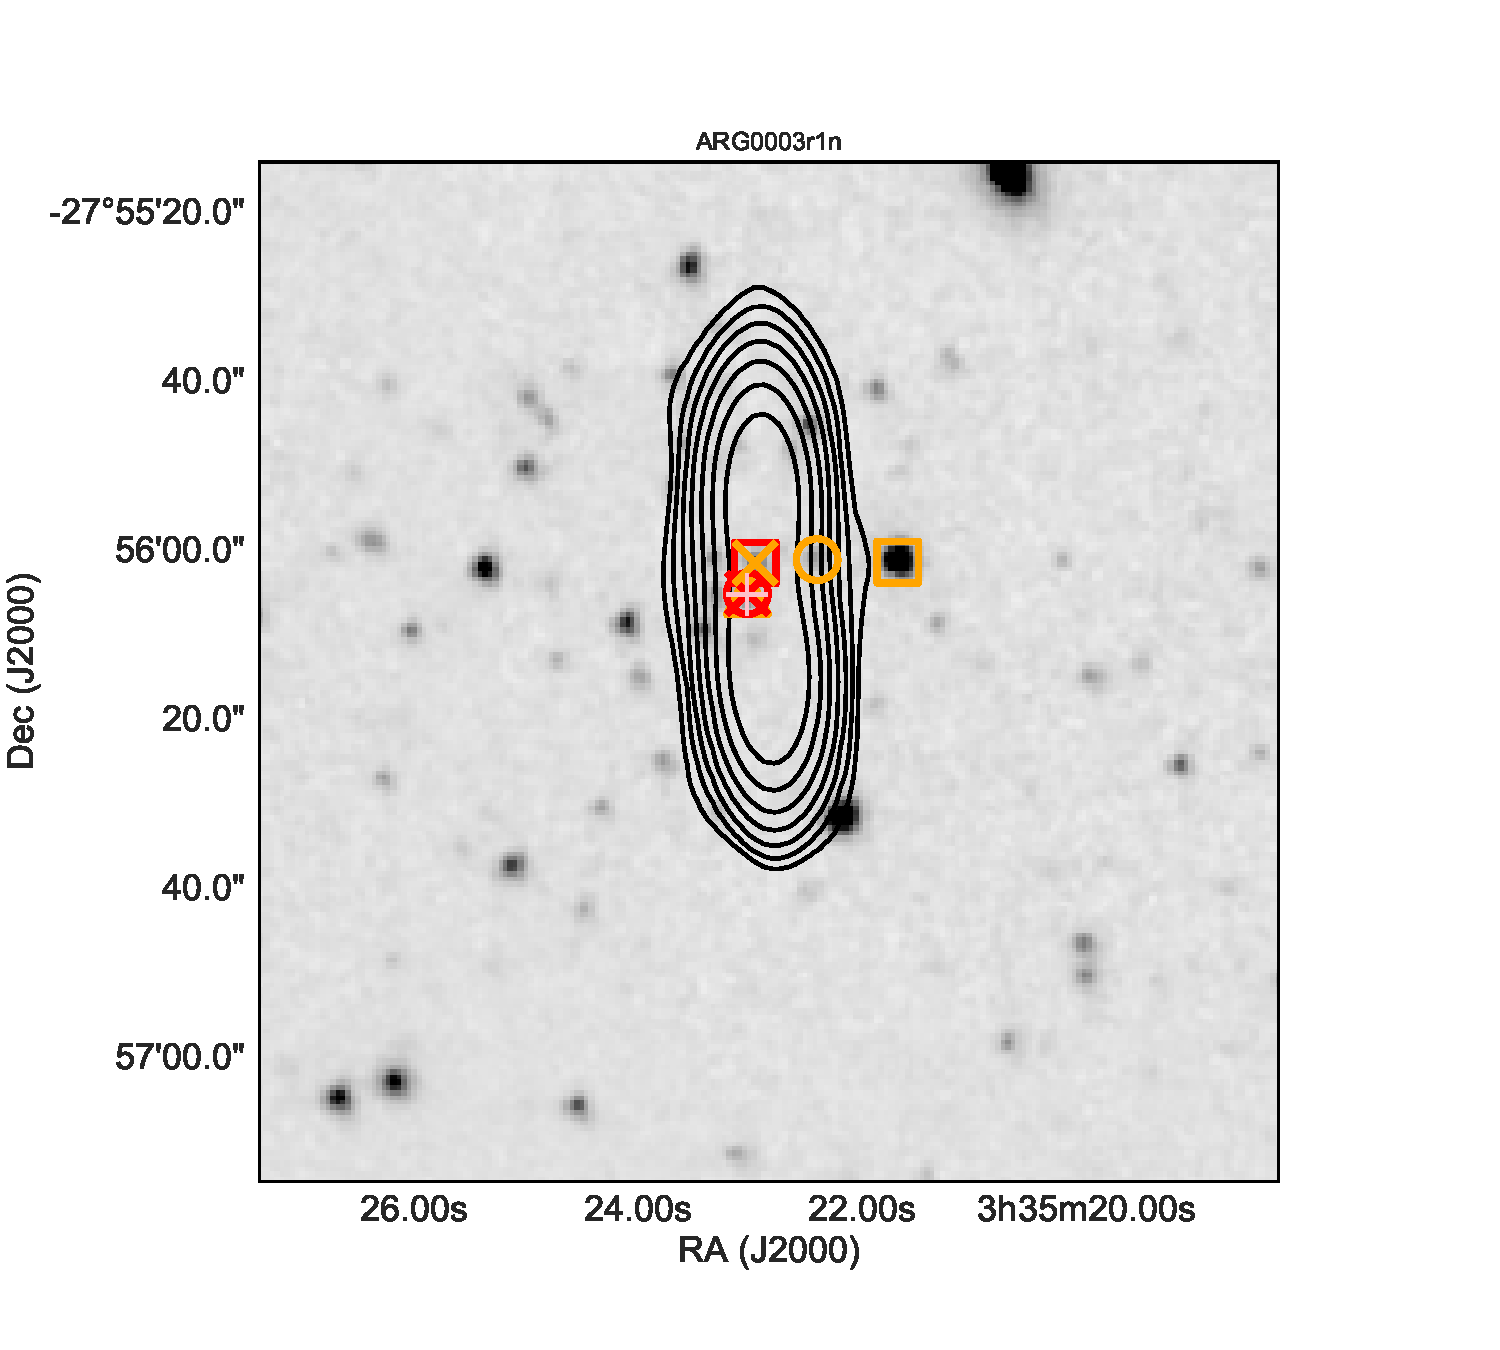
\includegraphics[trim={0cm 1cm 3.5cm 2.5cm}, clip, width=0.33\textwidth]{images/example_15_454.pdf}}%
        % \subfloat[]{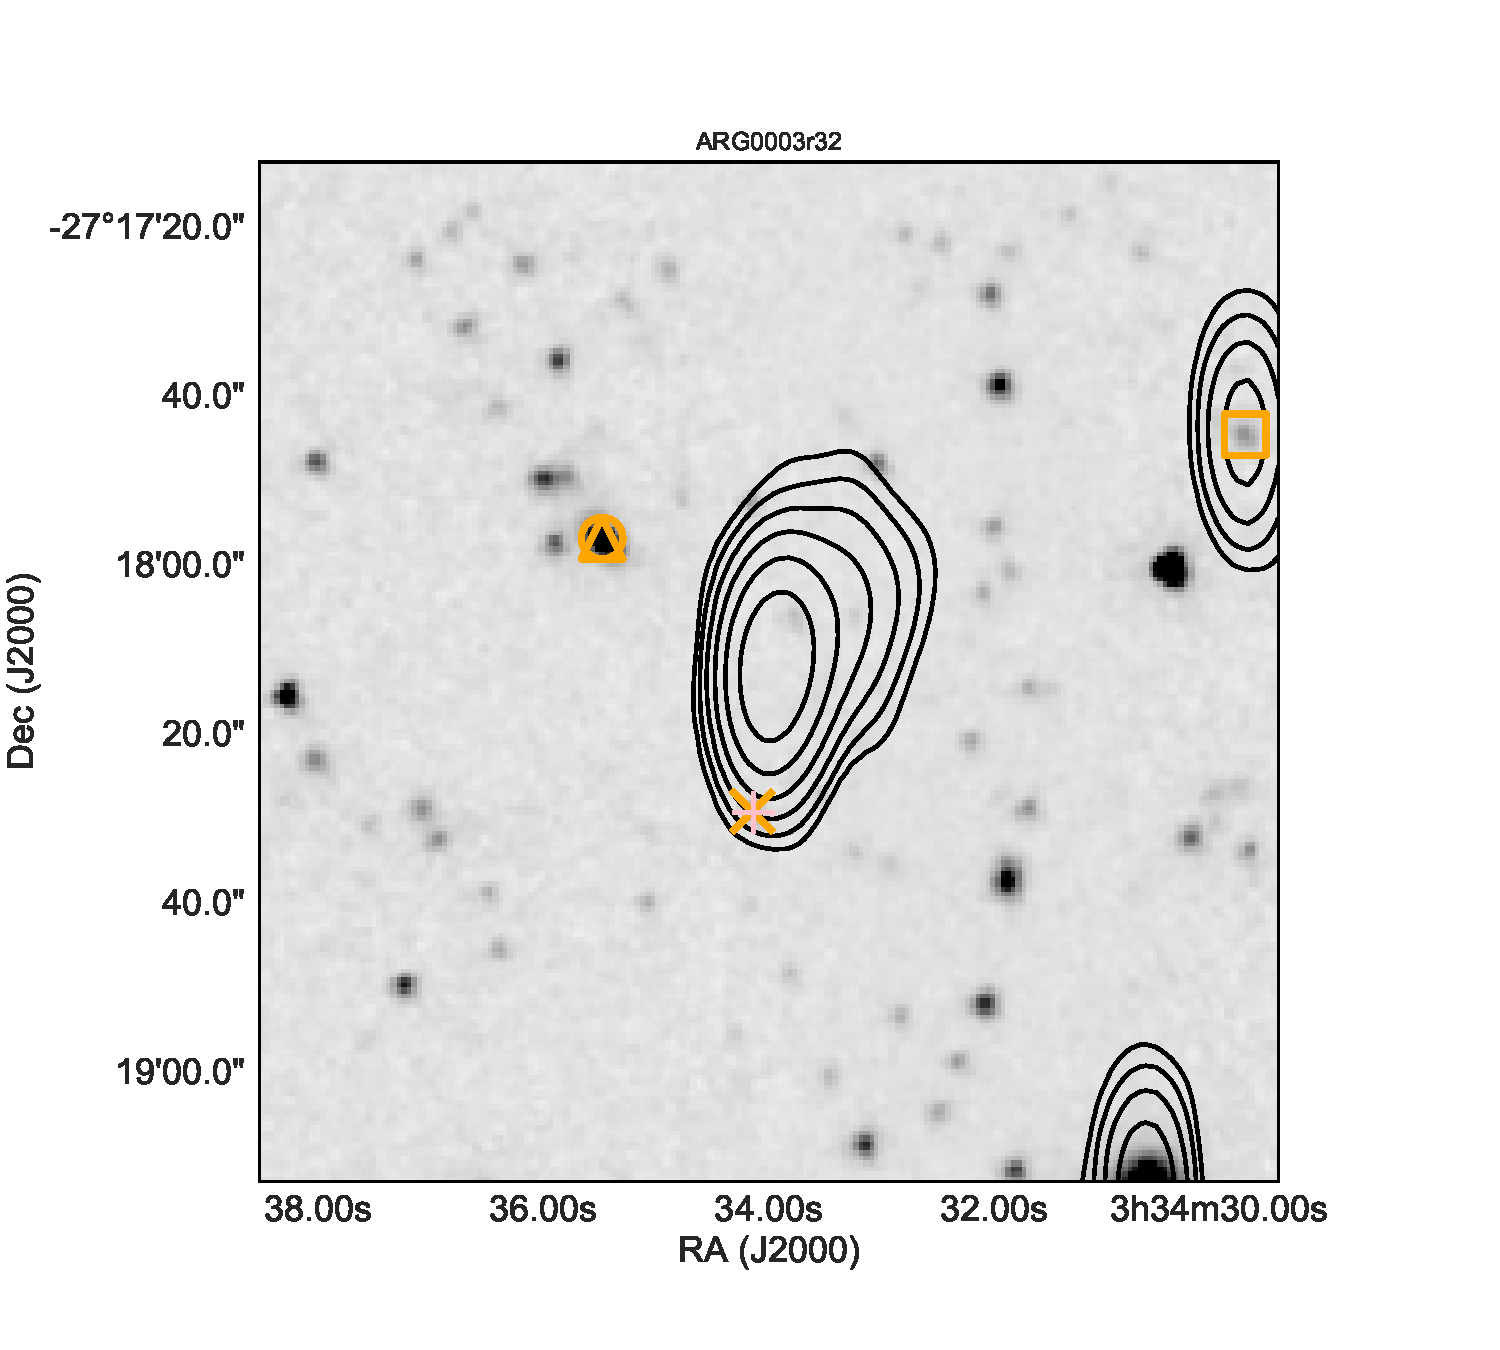
\includegraphics[width=0.25\textwidth]{images/example_14_424.pdf}}%
        % \subfloat[]{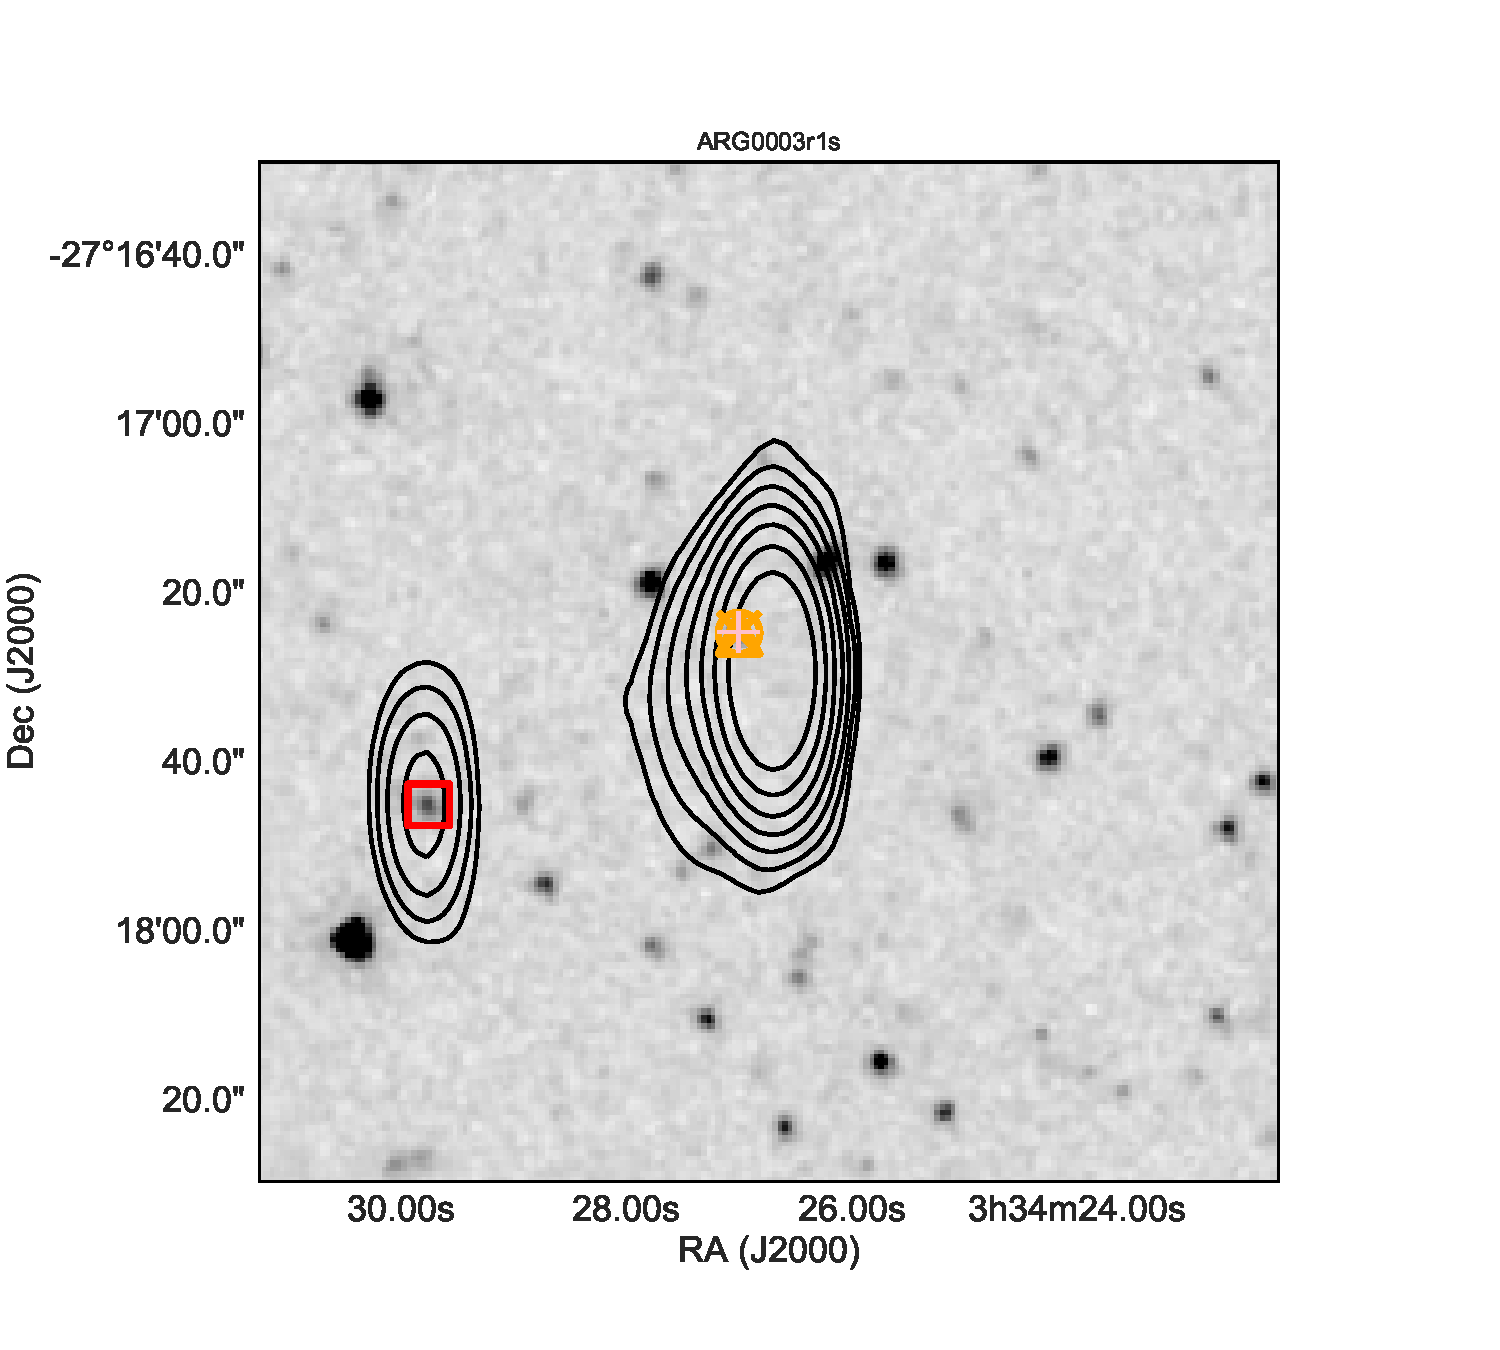
\includegraphics[width=0.25\textwidth]{images/example_13_415.pdf}}%
        \subfloat[]{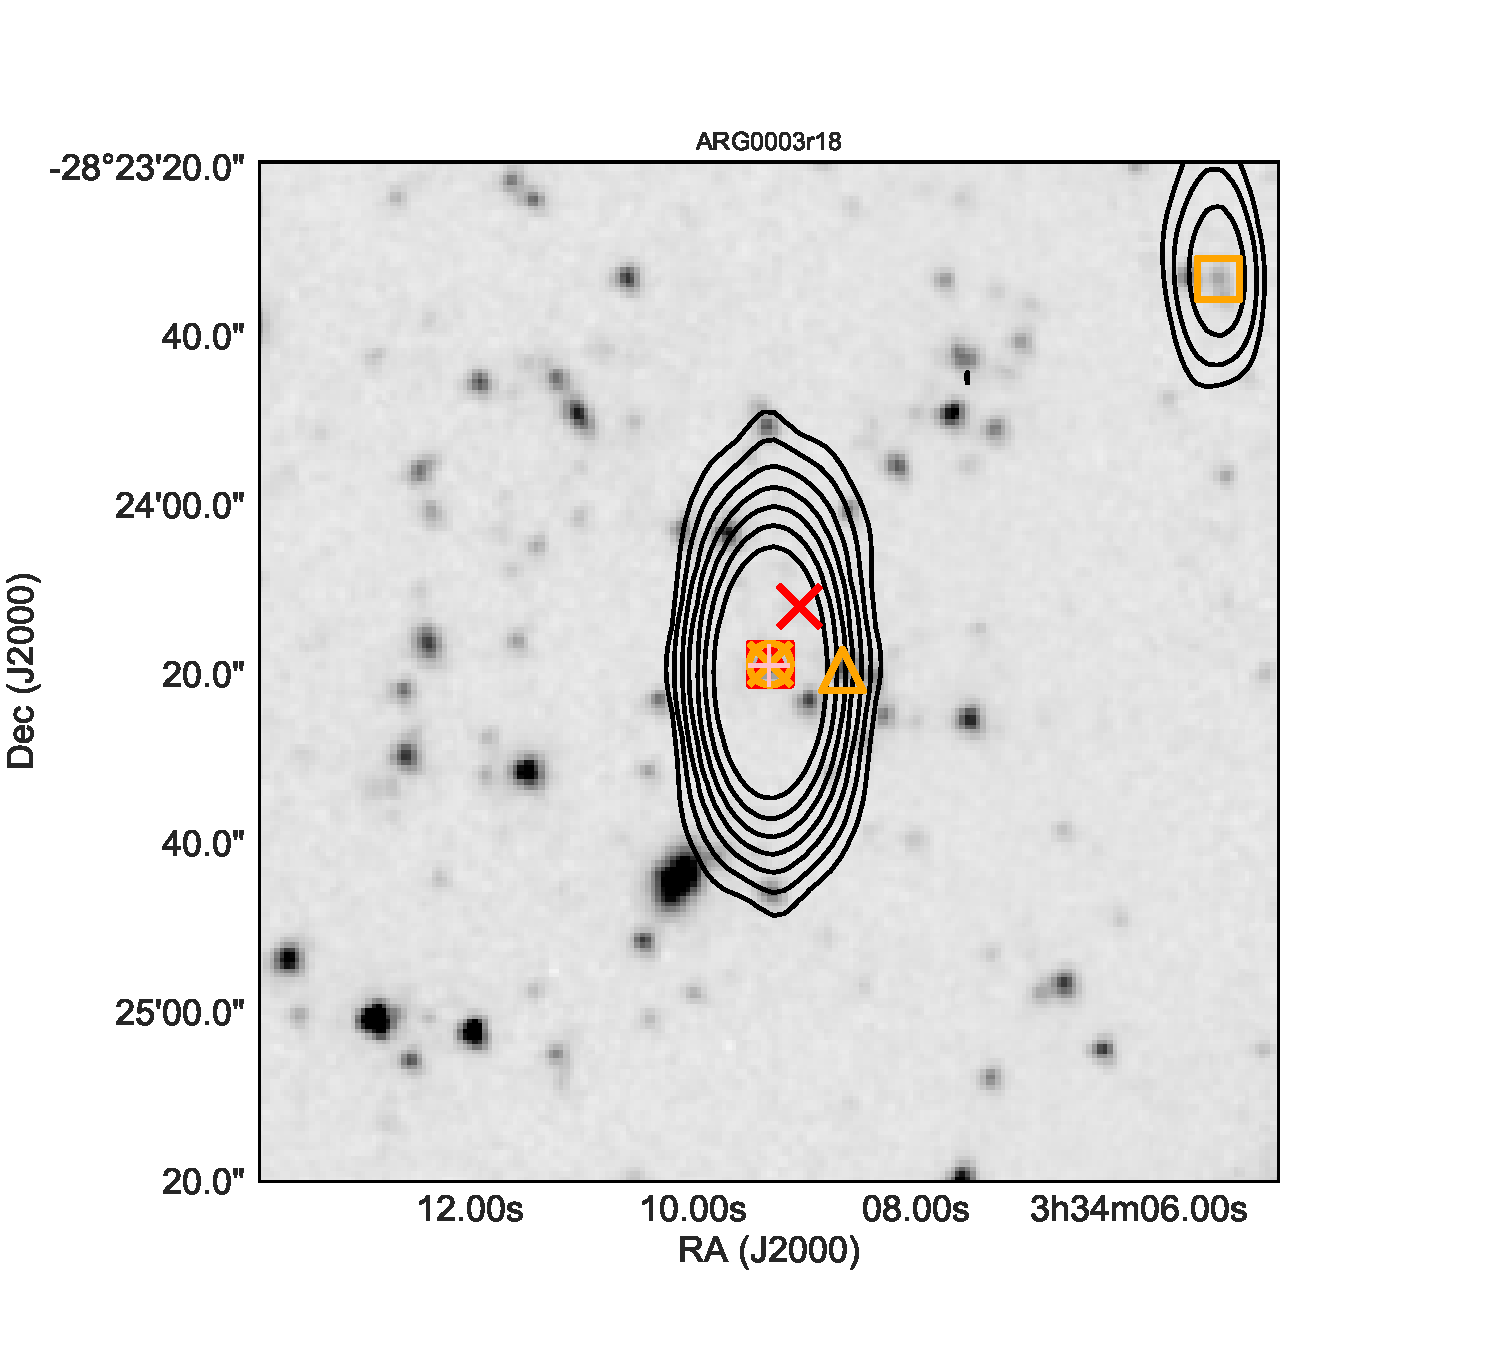
\includegraphics[trim={0cm 1cm 3.5cm 2.5cm}, clip, width=0.33\textwidth]{images/example_12_404.pdf}}%
        % \subfloat[]{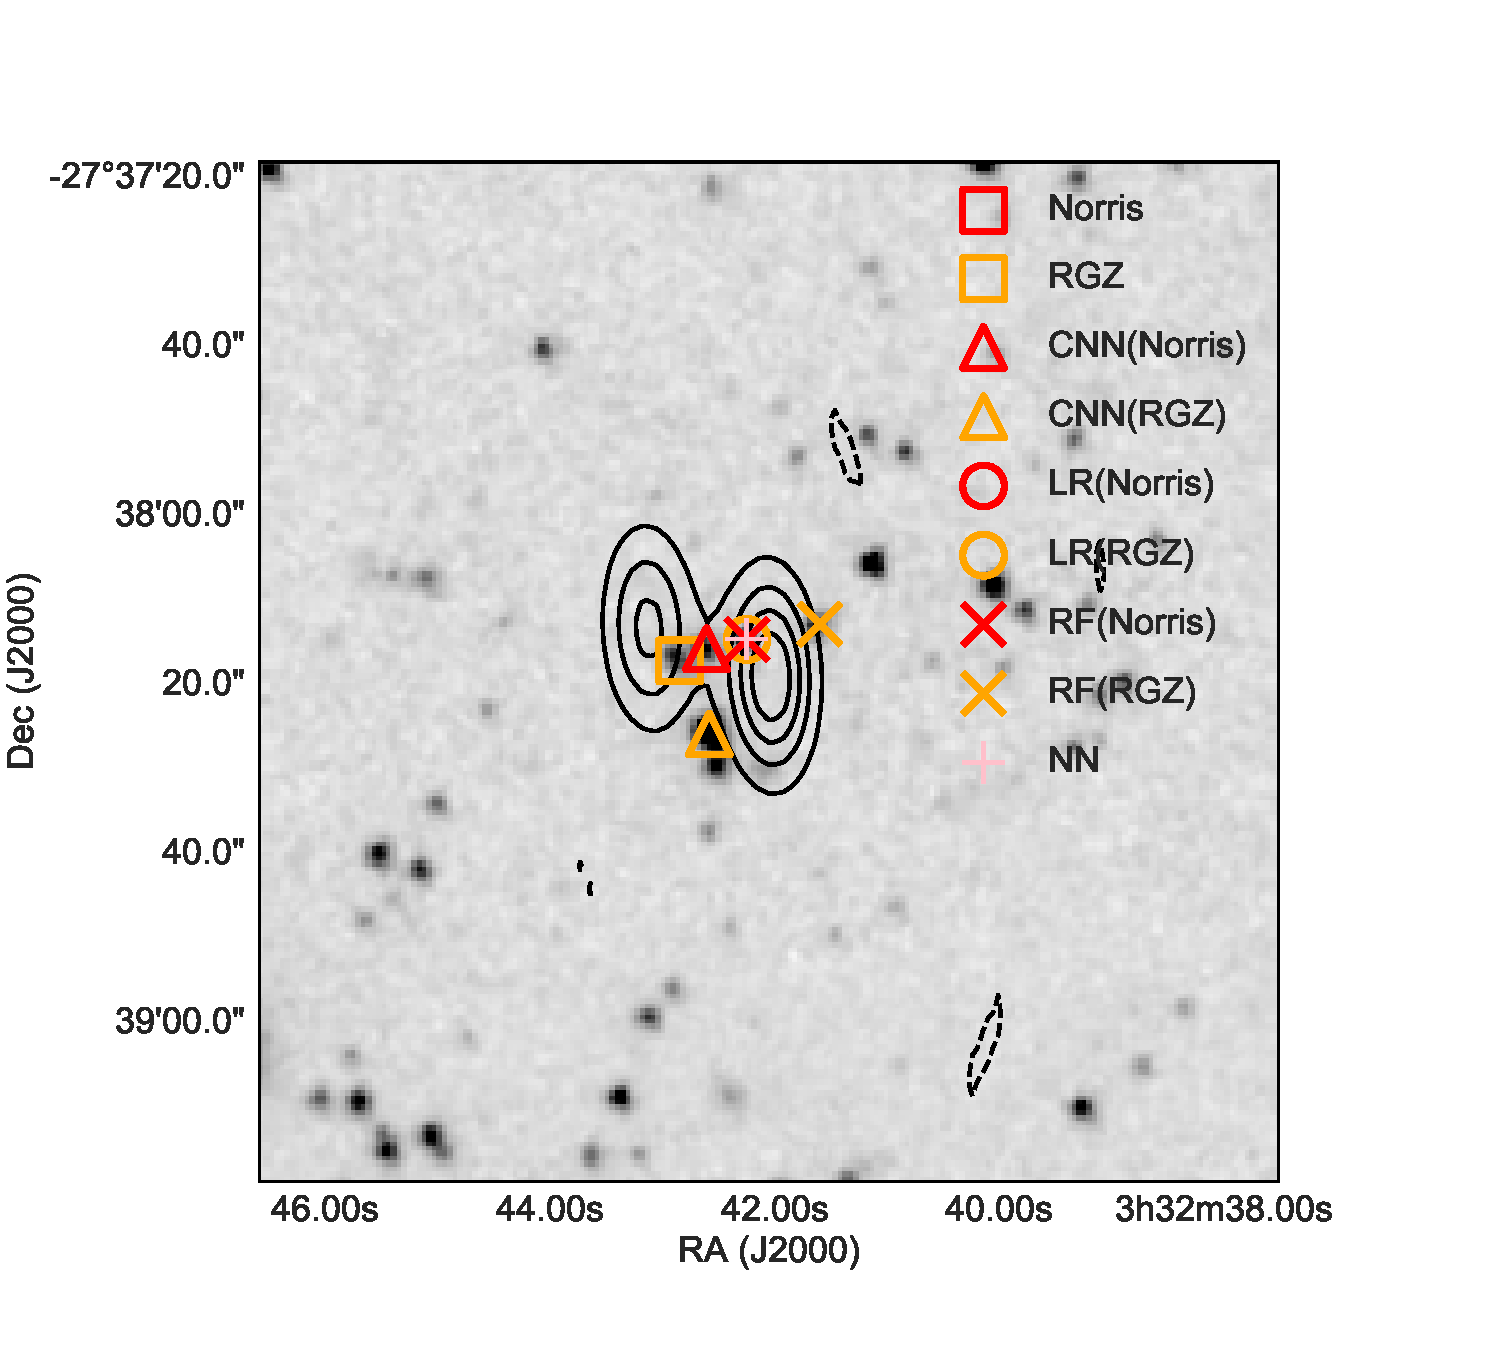
\includegraphics[width=0.25\textwidth]{images/example_11_306.pdf}}%
        \subfloat[]{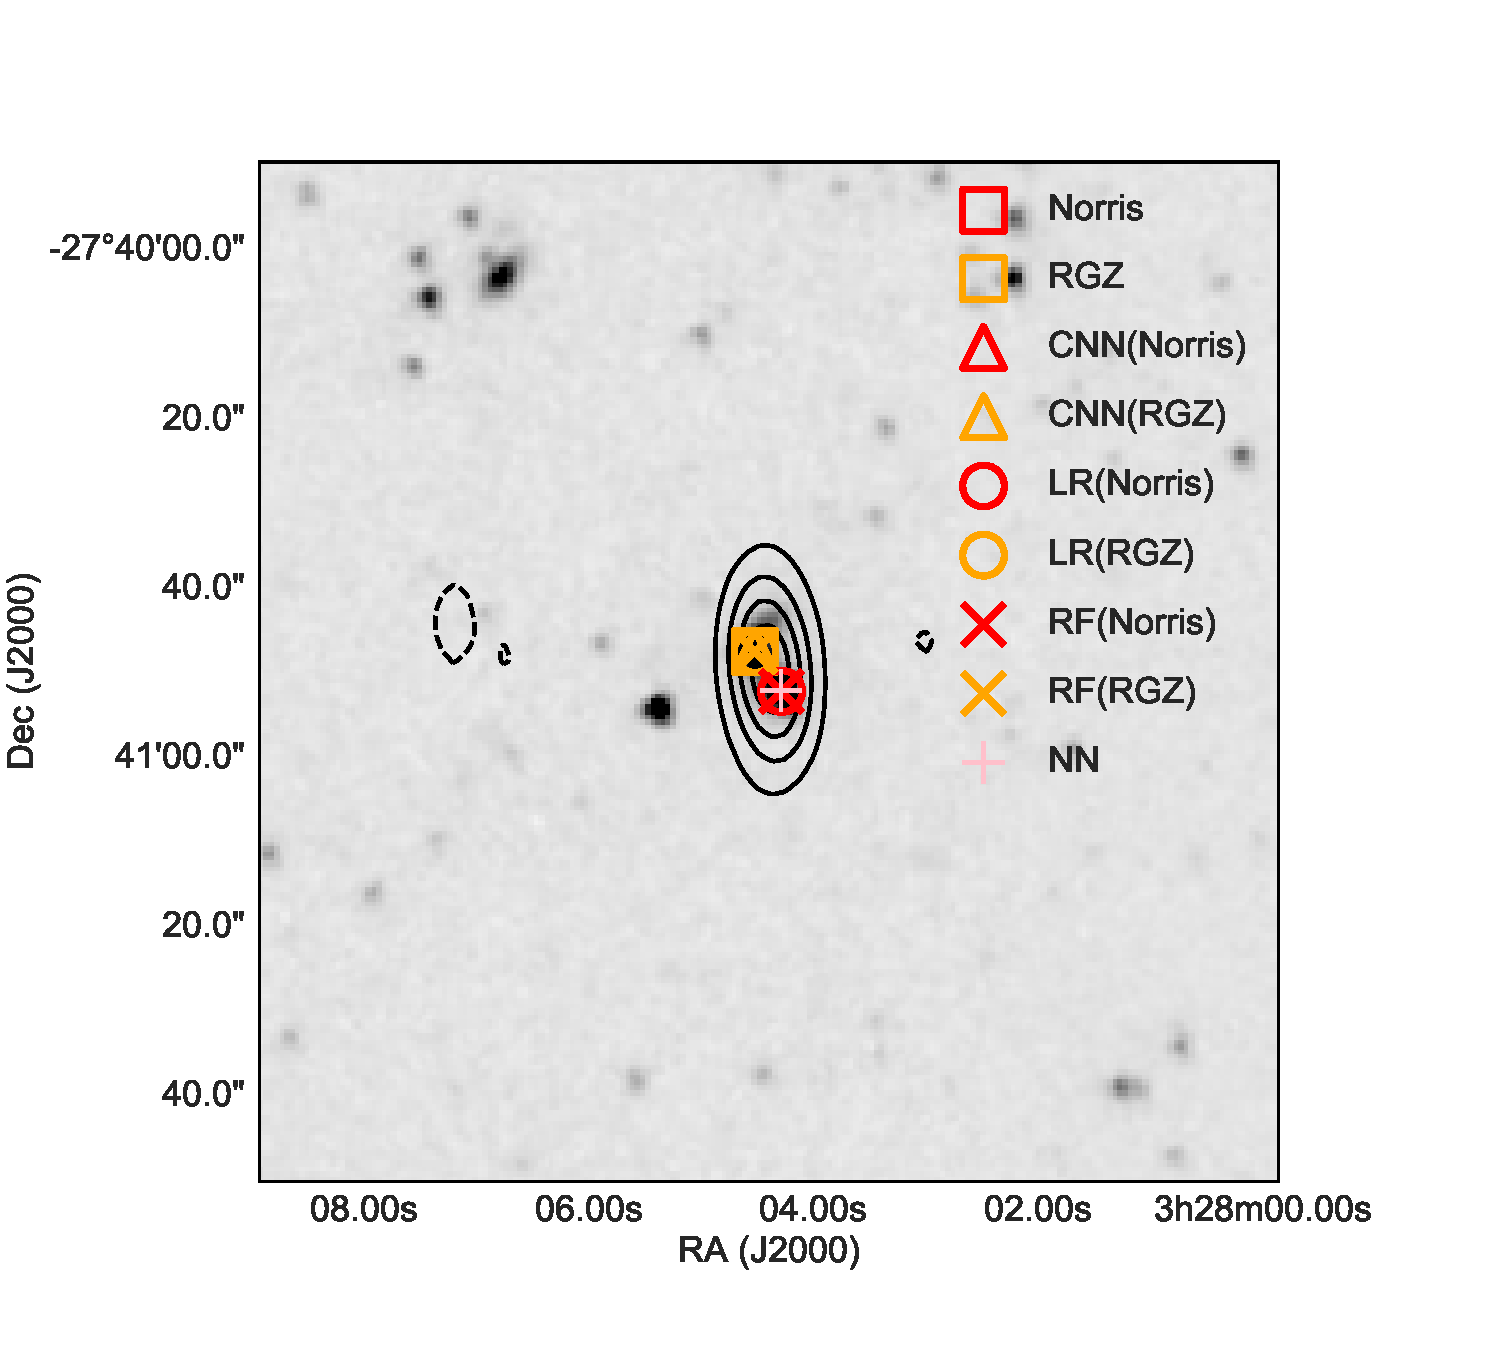
\includegraphics[trim={0cm 1cm 3.5cm 2.5cm}, clip, width=0.33\textwidth]{images/example_2_68.pdf}}

        % \subfloat[]{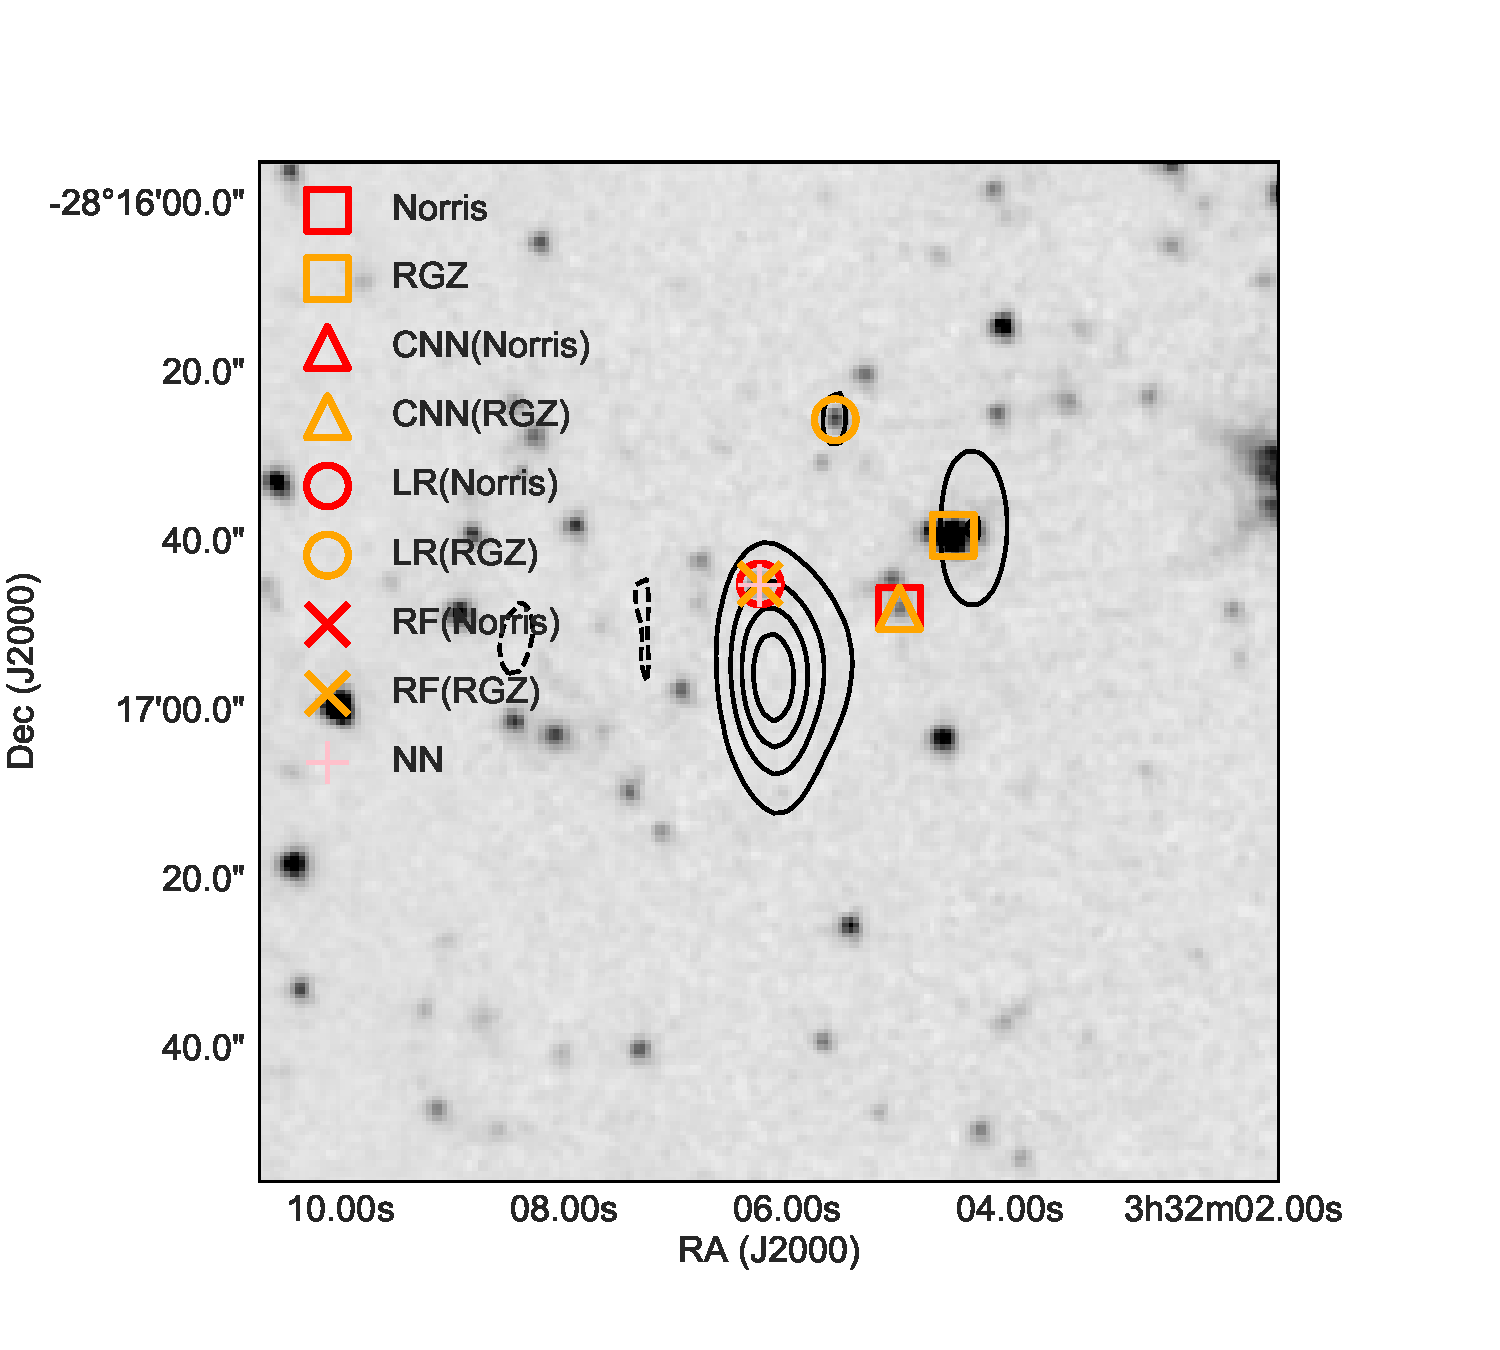
\includegraphics[width=0.25\textwidth]{images/example_9_264.pdf}}%
        % \subfloat[]{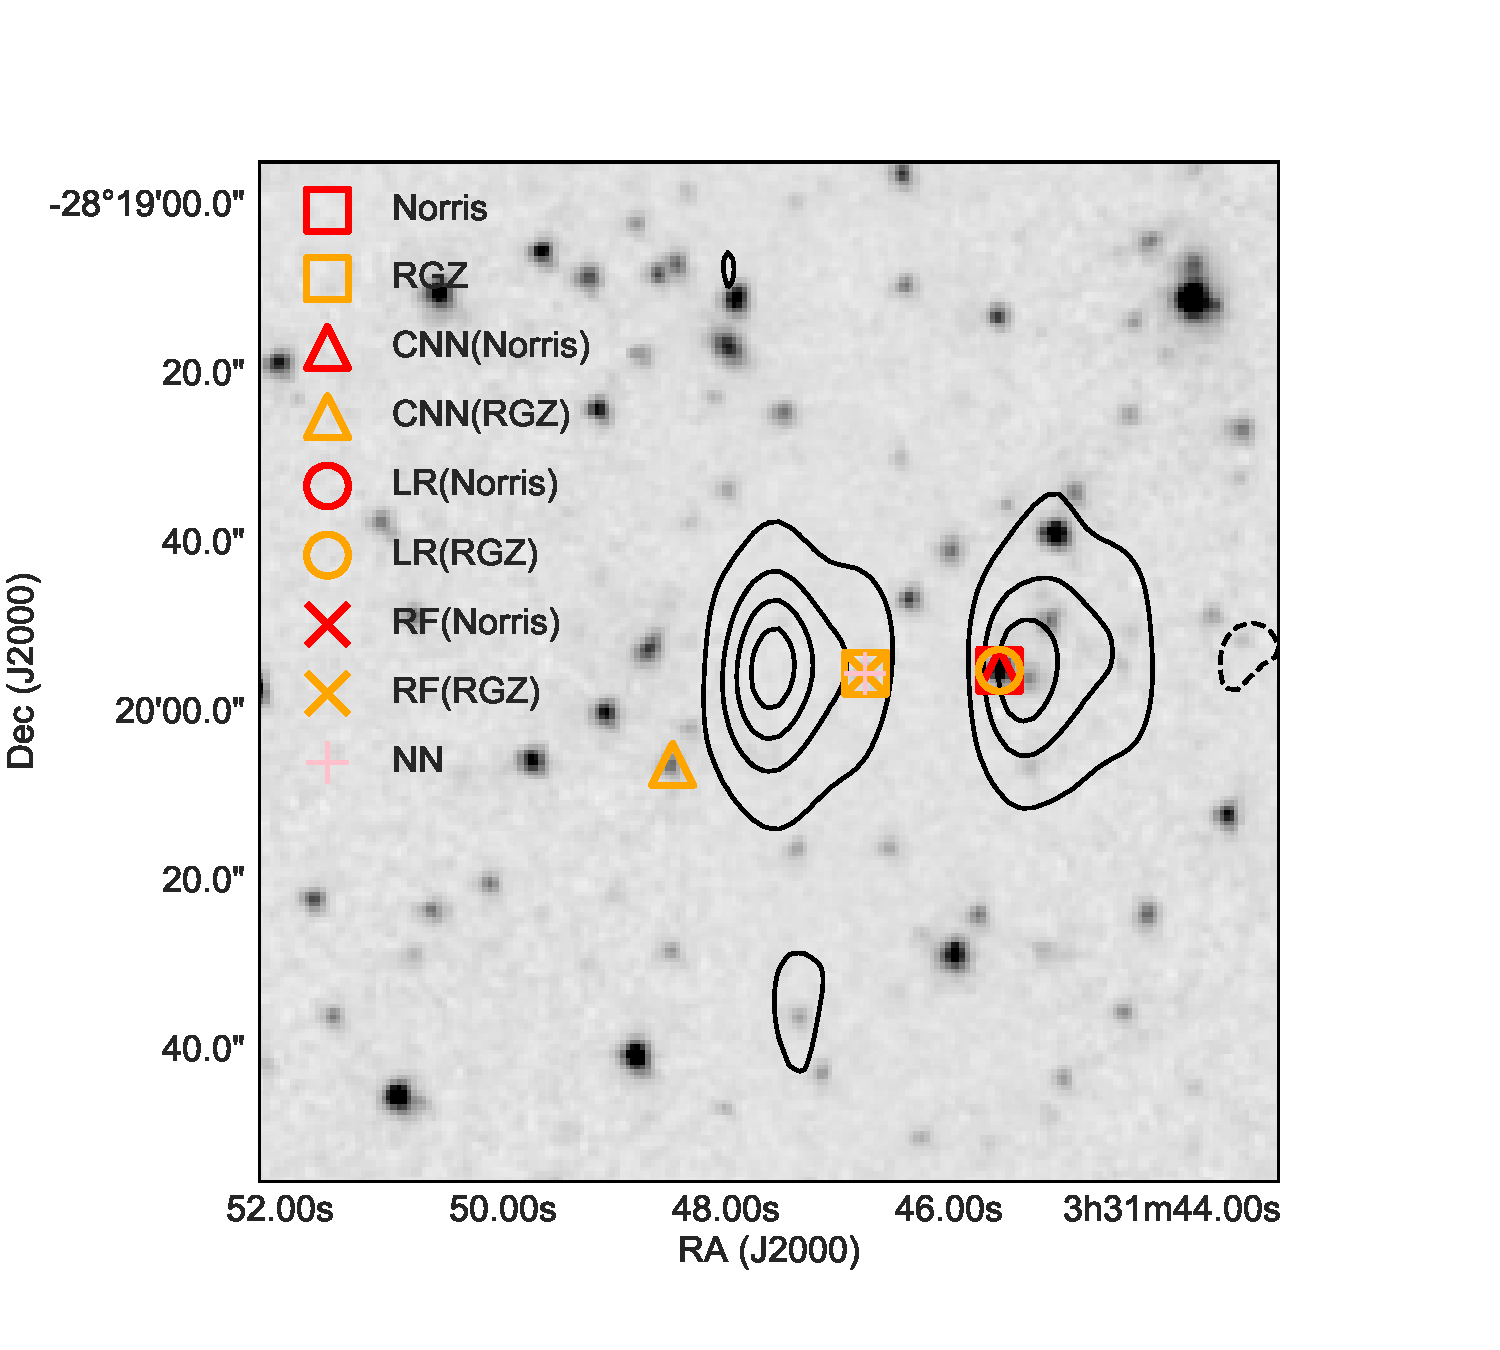
\includegraphics[width=0.25\textwidth]{images/example_8_239.pdf}}
        % \subfloat[]{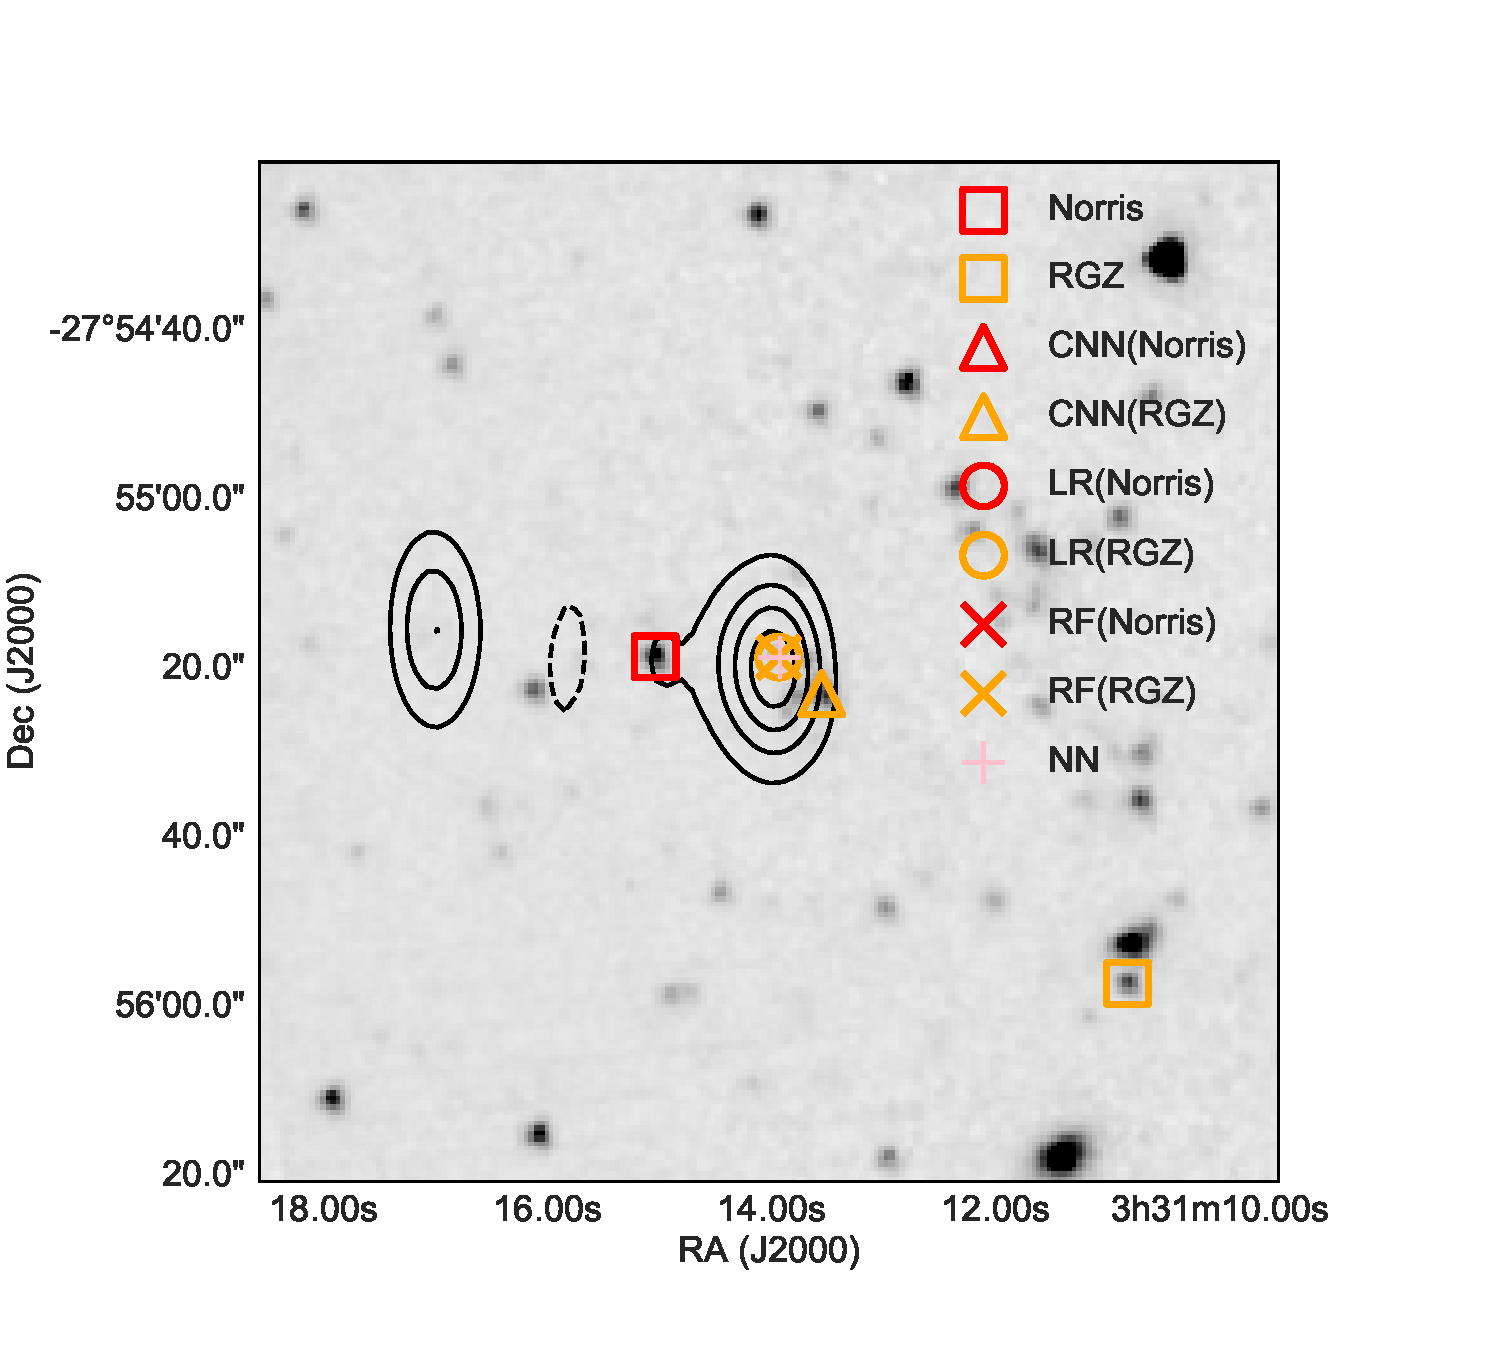
\includegraphics[width=0.25\textwidth]{images/example_7_207.pdf}}%
        % \subfloat[]{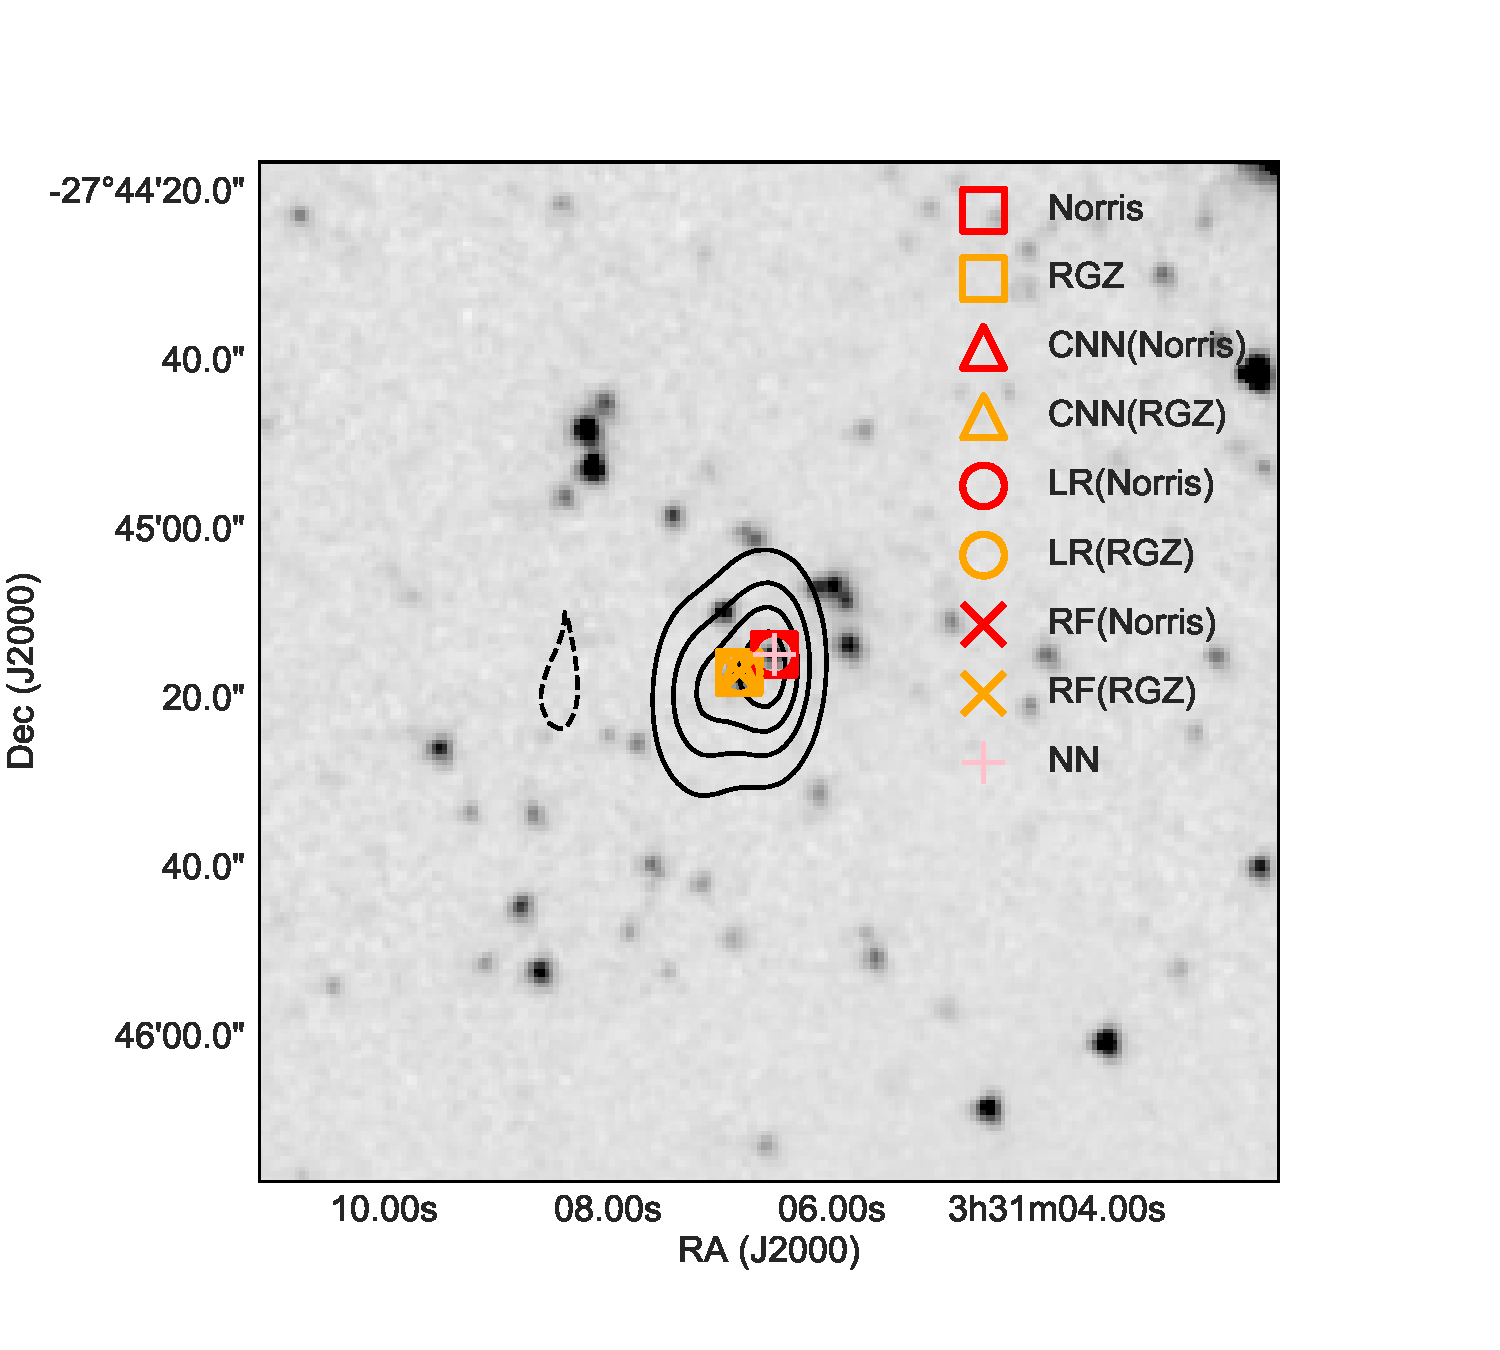
\includegraphics[width=0.25\textwidth]{images/example_6_197.pdf}}%
        % \subfloat[]{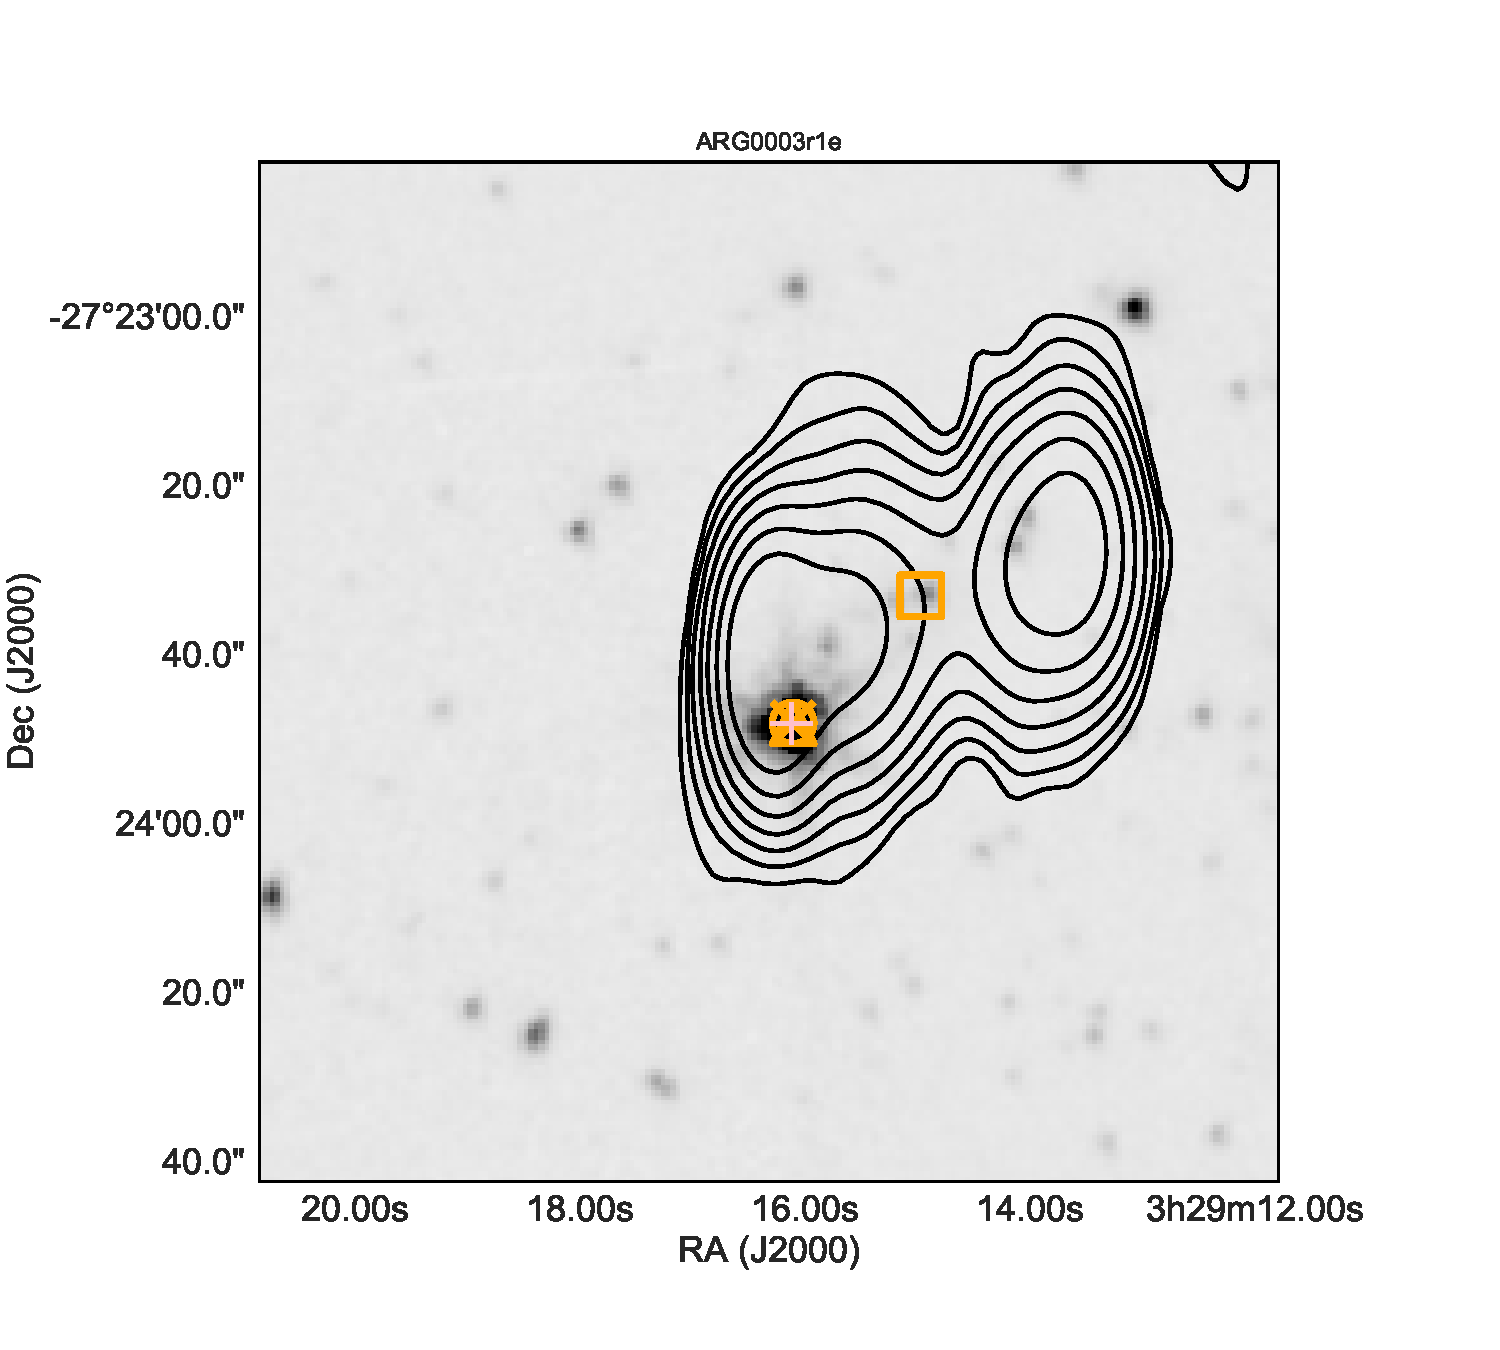
\includegraphics[width=0.25\textwidth]{images/example_5_113.pdf}}%
        \subfloat[]{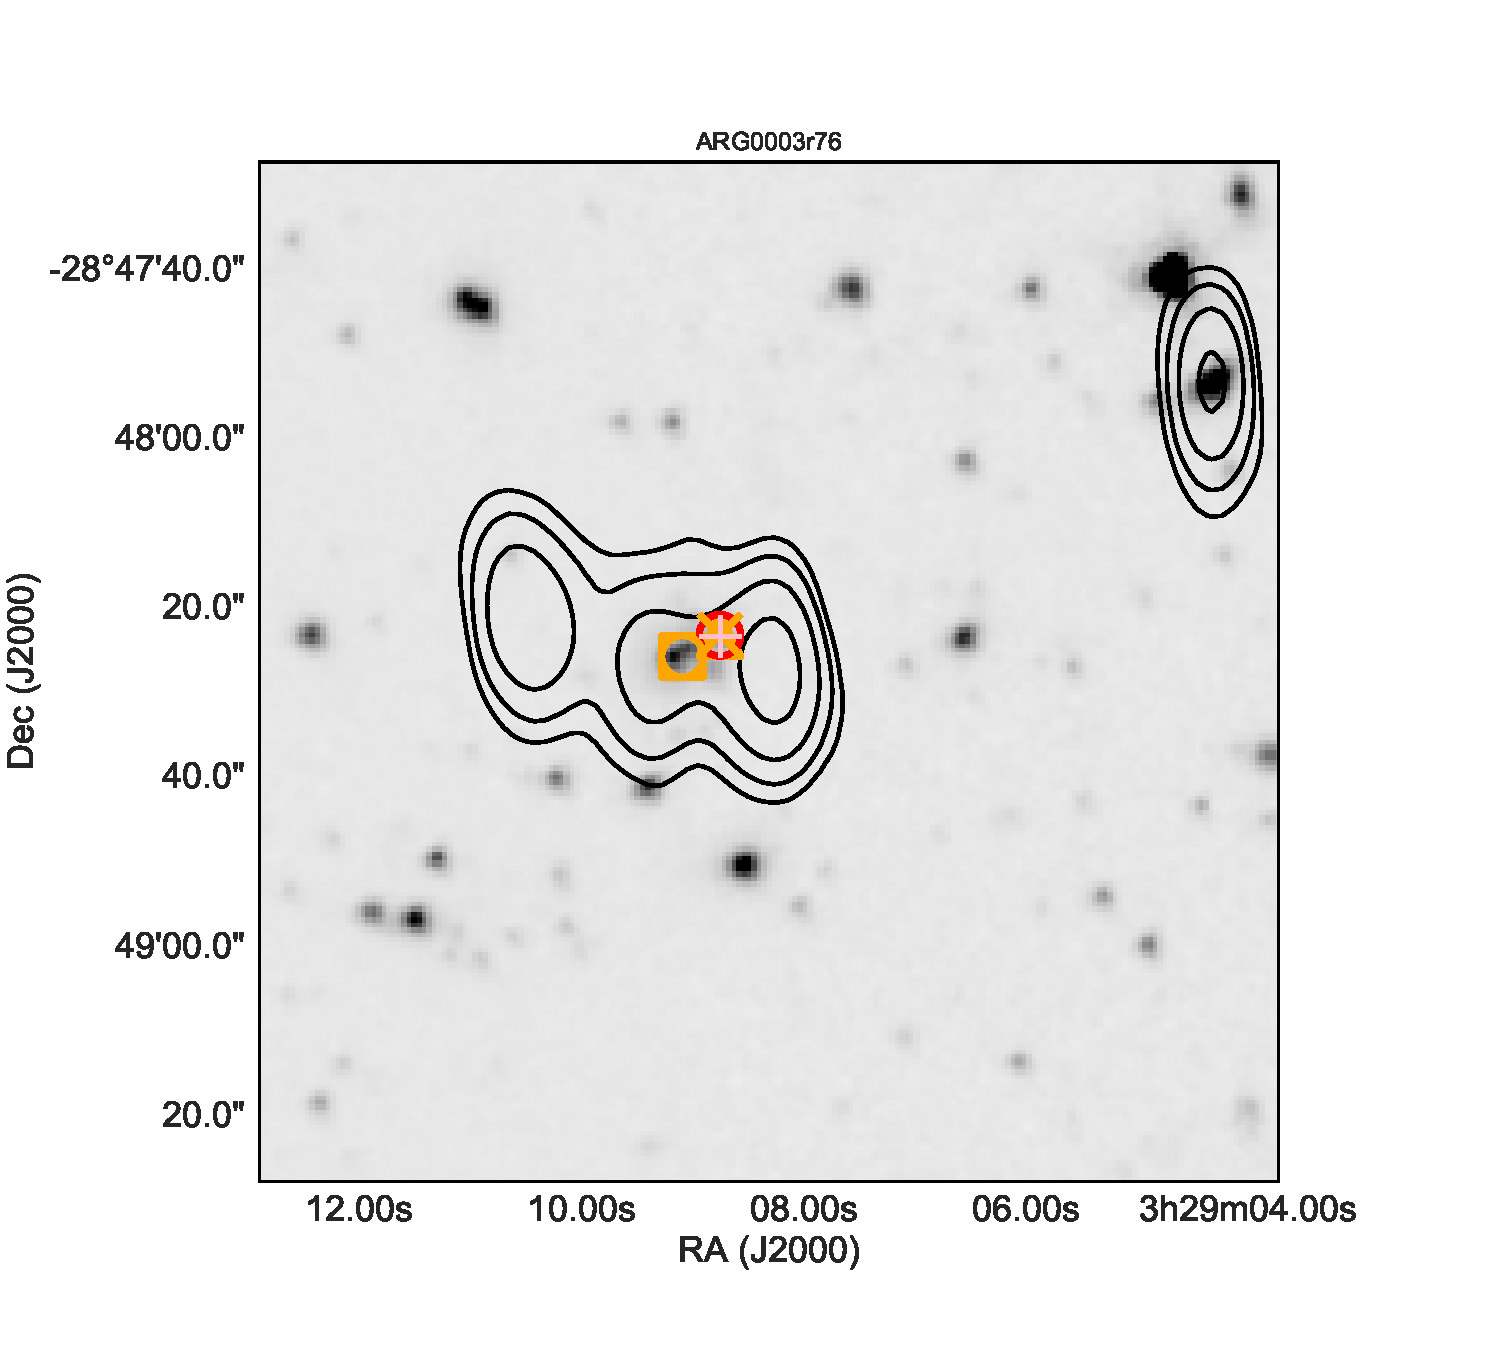
\includegraphics[trim={0cm 1cm 3.5cm 2.5cm}, clip, width=0.33\textwidth]{images/example_4_106.pdf}}%
        % \subfloat[]{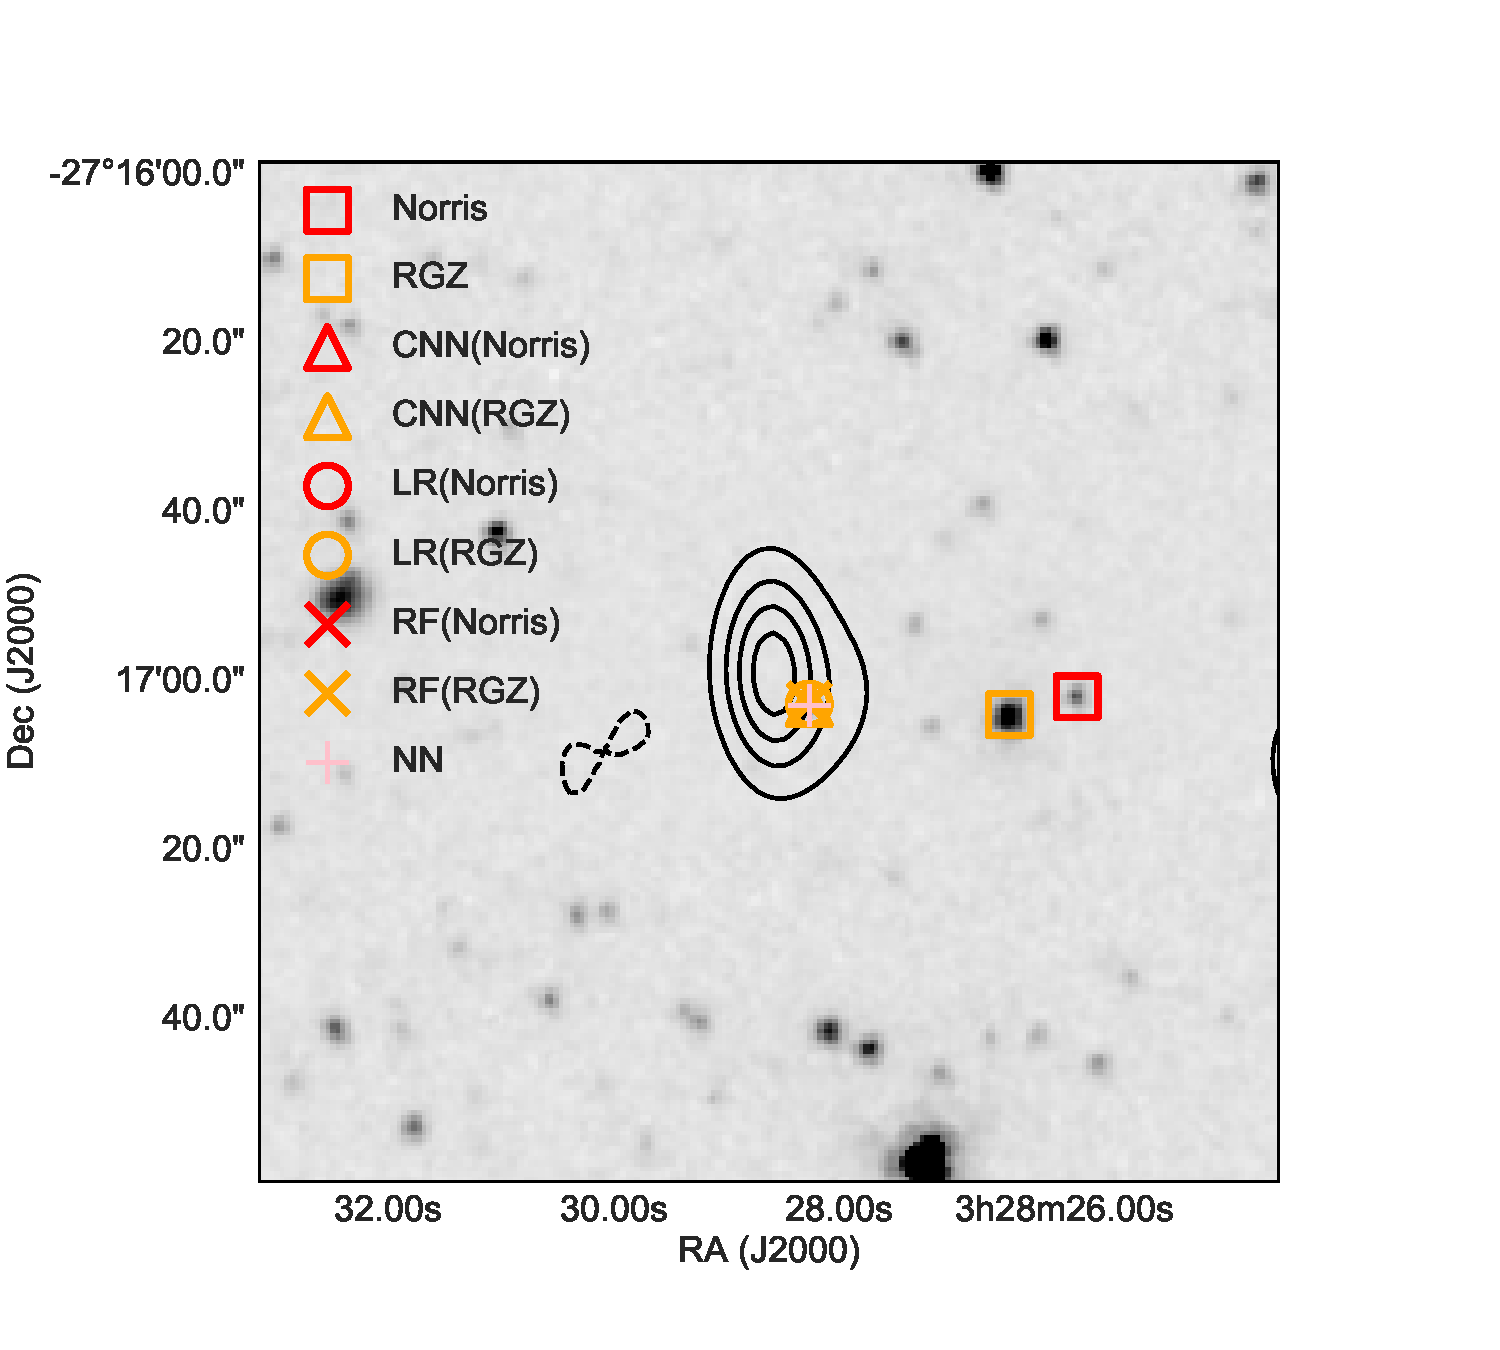
\includegraphics[width=0.25\textwidth]{images/example_3_86.pdf}}%
        \subfloat[]{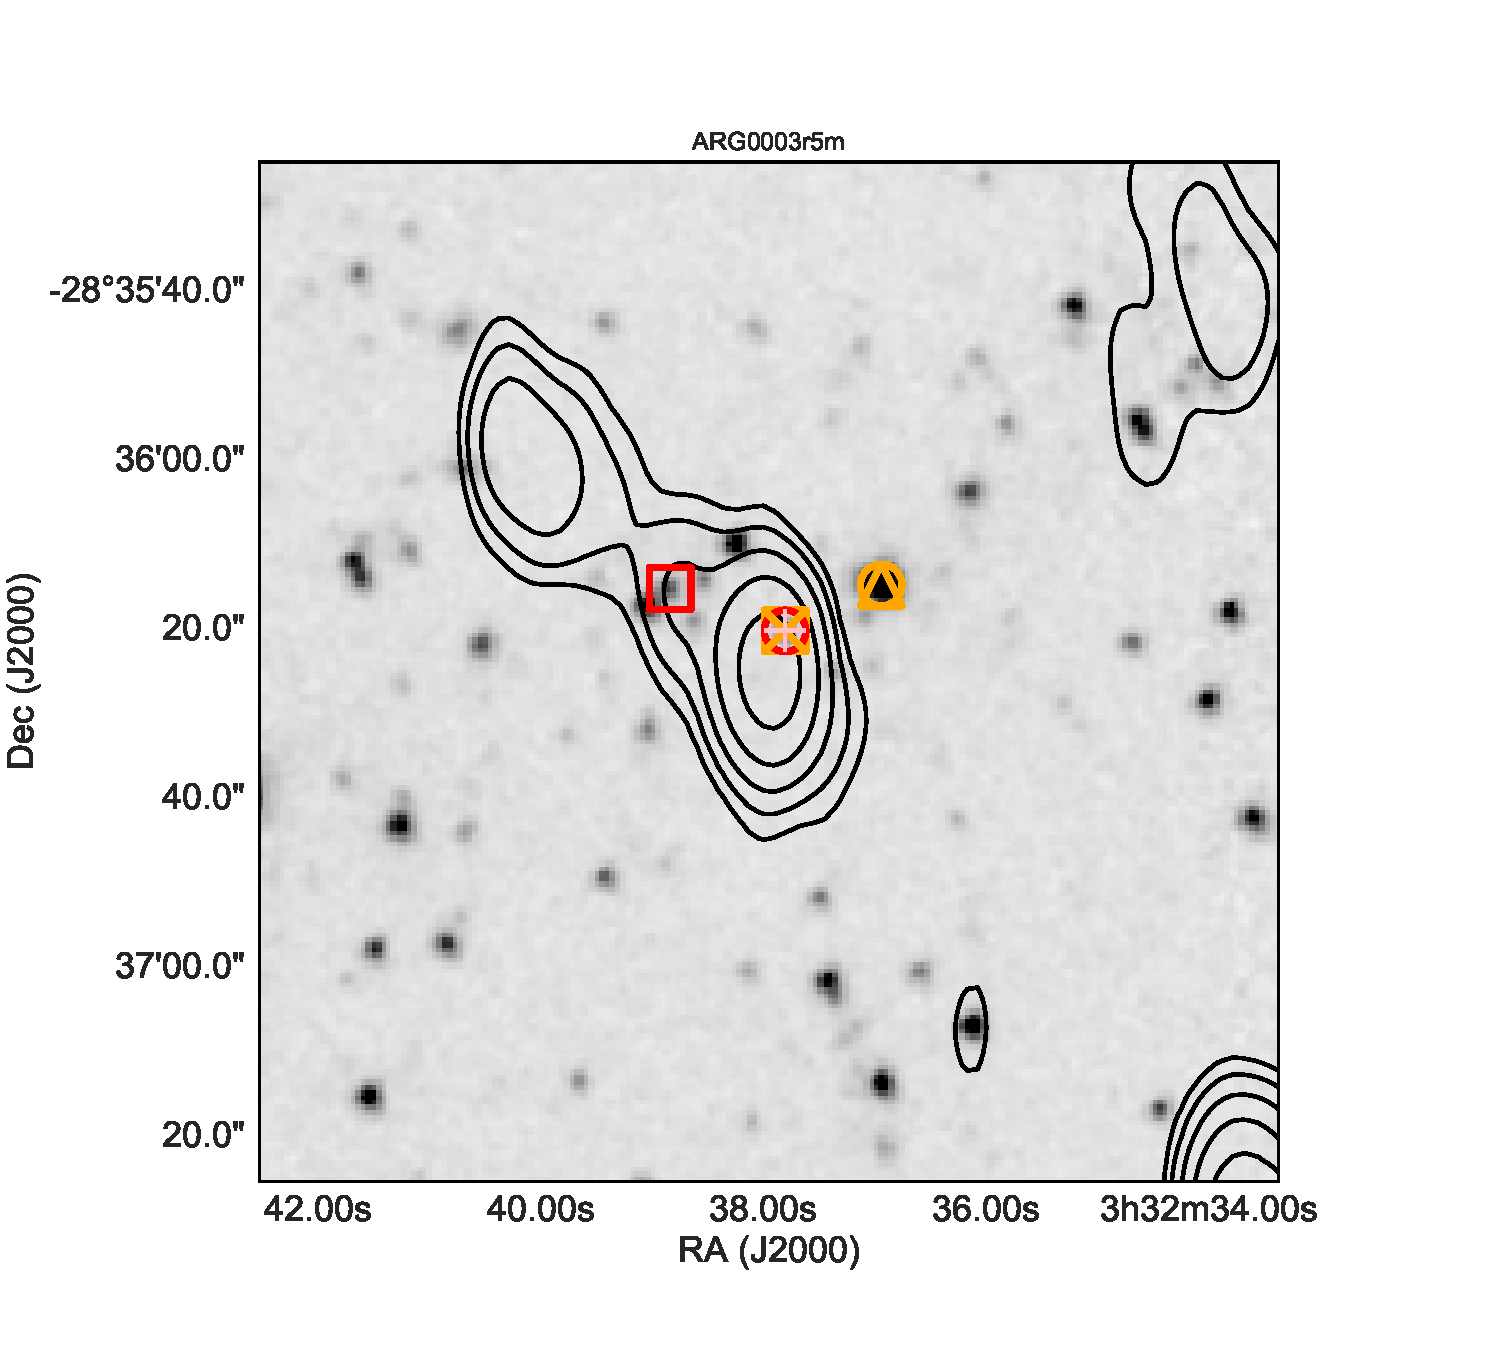
\includegraphics[trim={0cm 1cm 3.5cm 2.5cm}, clip, width=0.33\textwidth]{images/example_10_298.pdf}}%
        % \subfloat[]{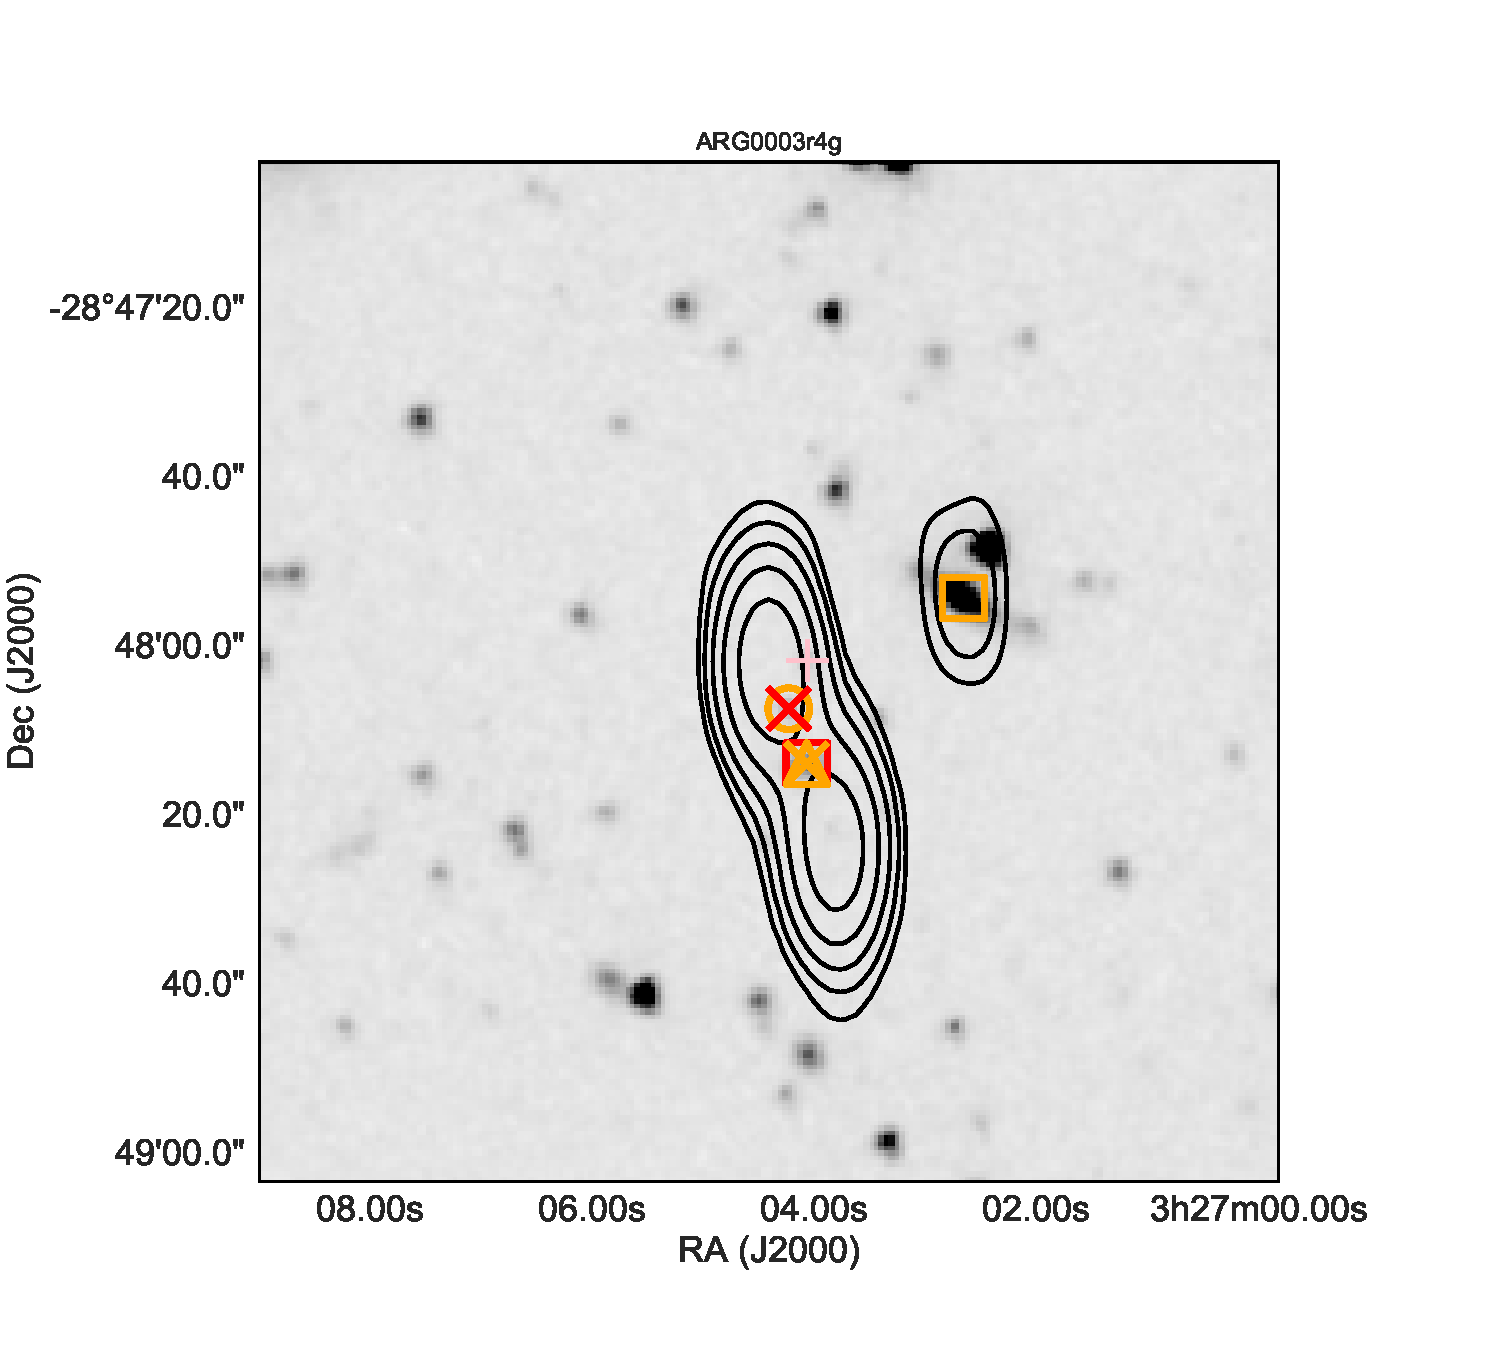
\includegraphics[width=0.25\textwidth]{images/example_1_30.pdf}}%
        \subfloat[]{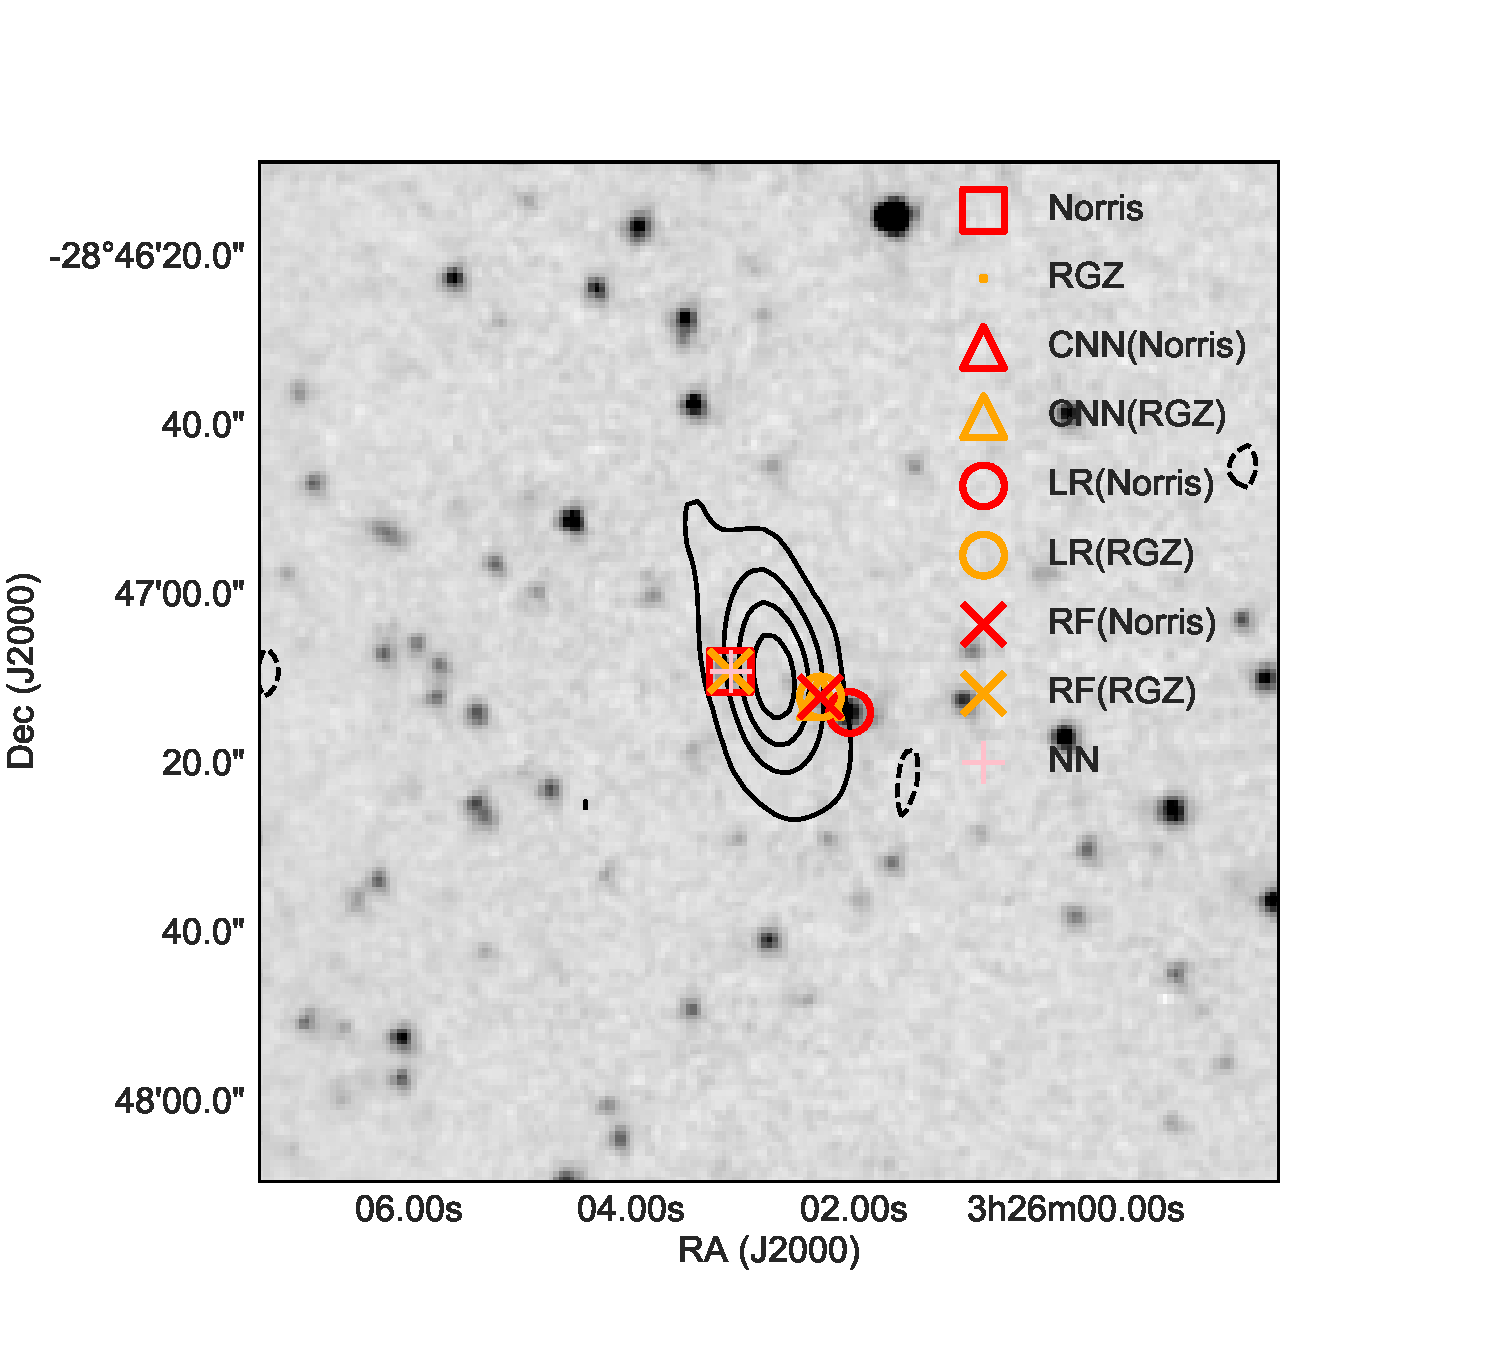
\includegraphics[trim={0cm 1cm 3.5cm 2.5cm}, clip, width=0.33\textwidth]{images/example_0_0.pdf}}%
        \caption{\label{fig:examples} Examples of resolved sources where the incorrect cross-identification was selected by random forests trained on expert labels. Classifier/training set combinations are denoted $C(S)$ where $C$ is the classifier and $S$ is the training set. `LR' is logistic regression, `CNN' is convolutional neural networks, and `RF' is random forests. `Norris' refers to the expert labels and `RGZ' refers to the Radio Galaxy Zoo labels. The cross-identification made by nearest neighbours is shown by `NN'.}
    \end{figure*}

\subsection{Application to ATLAS-ELAIS}
  \label{sec:elais}

  \begin{figure}
  \centering
  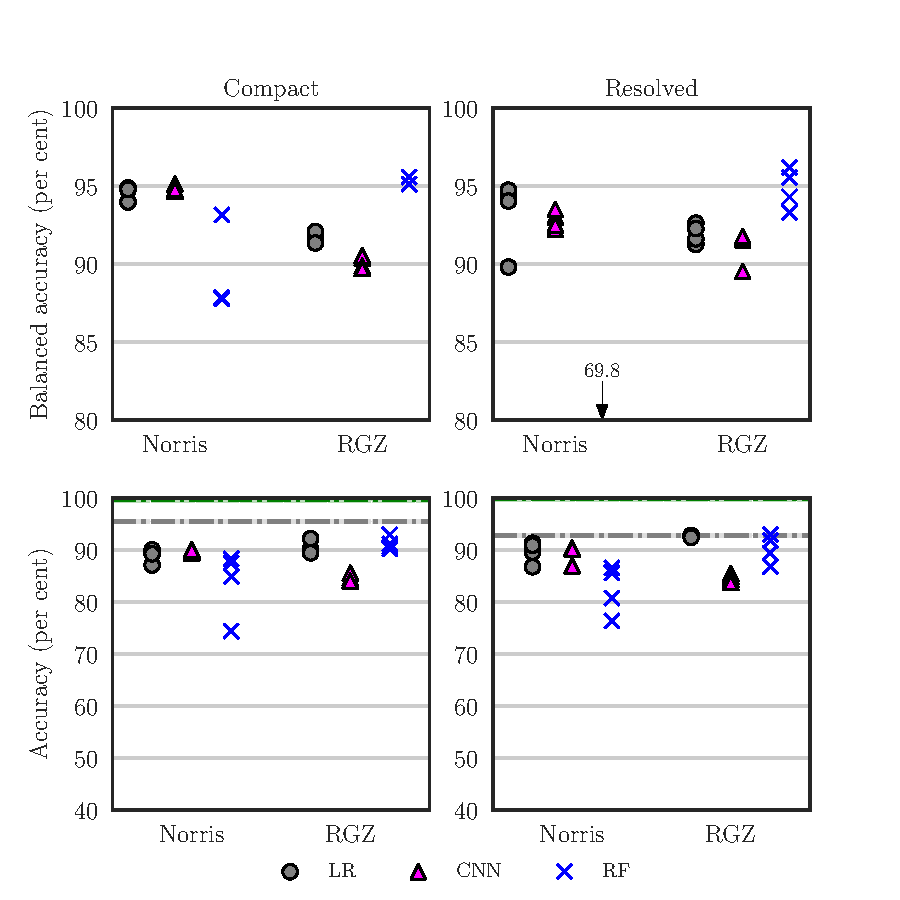
\includegraphics[width=\columnwidth]{images/elais-grid-new.pdf}
  \caption{Performance of different classifiers trained on CDFS and tested on resolved and compact sources in ELAIS-S1. Points represent classifiers trained on different quadrants of CDFS, with markers and axes as in \autoref{fig:ba}. The balanced acccuracy of expert-trained random forest classifiers falls below the axis and the corresponding mean accuracy is shown by an arrow. The solid green line indicates the X-ID performance of a `perfect' classifier; this is almost 100 per cent. The grey dashed line indicates the X-ID performance of nearest neighbours. Note that the pipeline in \autoref{fig:flowchart} is not used in this figure.
    \label{fig:elais-ba}}
  \end{figure}

  \begin{figure}
    \centering
    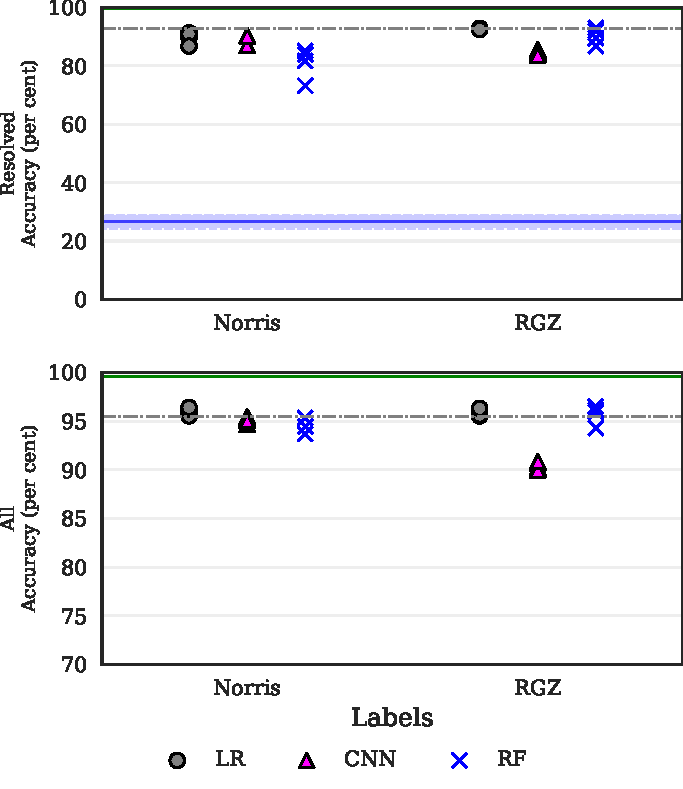
\includegraphics[width=0.9\columnwidth]{images/elais_cross_identification_grid.pdf}
    \caption{Performance of different classifiers trained on CDFS and tested on ELAIS-S1. Markers are as in \autoref{fig:cross-id-accuracy} and horizontal lines are as in \autoref{fig:elais-ba}. Note that the pipeline in \autoref{fig:flowchart} is not used in this figure.
      \label{fig:elais-cross-id-accuracy}}
  \end{figure}

  We applied the classifiers trained on CDFS to perform cross-identification on the ELAIS-S1 field. Both CDFS and ELAIS-S1 were imaged by the same radio telescope to similar sensitivities and angular resolution for the ATLAS survey. As ELAIS-S1 has been cross-identified with SWIRE host galaxies by \citet{middelberg08}, we can use these cross-identifications to derive another set of expert labels, and hence determine how accurate our method is. If our method generalises well across different parts of the sky, then we expect CDFS-trained classifiers applied to cross-identification in ELAIS-S1 to perform comparably to application to CDFS. In \autoref{fig:elais-ba} we plot the performance of CDFS-trained logistic regression, random forests, and convolutional neural networks on both the galaxy classification task and the cross-identification task for resolved and compact sources. We also plot the accuracy of a nearest-neighbours approach. In \autoref{fig:elais-cross-id-accuracy} we plot the performance of these classifiers on the full set of ATLAS~DR1 radio components using the pipeline in \autoref{fig:flowchart}. We list the corresponding accuracies in the supplement.

  Cross-identification results from ELAIS-S1 are similar to those for CDFS,
  showing that classifiers trained on CDFS perform reasonably well on
  ELAIS-S1. However, nearest neighbours outperforms most methods on ELAIS-S1.
  This is likely because there is a much higher percentage of compact objects in ELAIS-S1 than in CDFS. The maximum achievable accuracy we have estimated for ELAIS-S1 is very close to 100 per cent, so (as for CDFS) a very accurate binary classifier would outperform nearest neighbours.

  One interesting difference between the ATLAS fields is that random forests trained on expert labels perform well on CDFS but poorly on ELAIS-S1. This is not the case for logistic regression or convolutional neural networks trained on expert labels, nor is it the case for random forests trained on Radio Galaxy Zoo. We hypothesise that this is because the ELAIS-S1 cross-identification catalogue \citep{middelberg08} labelled fainter radio components than the CDFS cross-identification catalogue \citep{norris06} due to noise from the very bright source ATCDFS\textunderscore{}J032836.53-284156.0 in CDFS. Classifiers trained on CDFS expert labels may thus be biased toward brighter radio components compared to ELAIS-S1. Radio Galaxy Zoo uses the third data release of ATLAS \citep{franzen15} and so classifiers trained on the Radio Galaxy Zoo labels may be less biased toward brighter sources compared to those trained on the expert labels. To test this hypothesis we tested each classifier against test sets with a signal-to-noise ratio (SNR) cutoff. A SWIRE object was only included in the test set for a given cutoff if it was located within $1'$ of a radio component with a SNR above the cutoff. The balanced accuracies for each classifier at each cutoff are shown in \autoref{fig:accuracies-flux}(a) and (b) and the distribution of test set size for each cutoff is shown in \autoref{fig:accuracies-flux}(c). \autoref{fig:accuracies-flux}(c) shows that ELAIS-S1 indeed has more faint objects than CDFS, with the SNR for which the two fields reach the same test set size (approximately $0.02$) indicated by the dashed vertical line on each plot. For CDFS, all classifiers perform reasonably well across cutoffs, with performance dropping as the size of the test set becomes small. For ELAIS-S1, logistic regression and convolutional neural networks perform comparably across all SNR cutoffs, but random forests do not: while random forests trained on Radio Galaxy Zoo labels perform comparably to other classifiers across all SNR cutoffs, random forests trained on expert labels show a considerable drop in performance below the dashed line.

  \begin{figure}
    \centering
    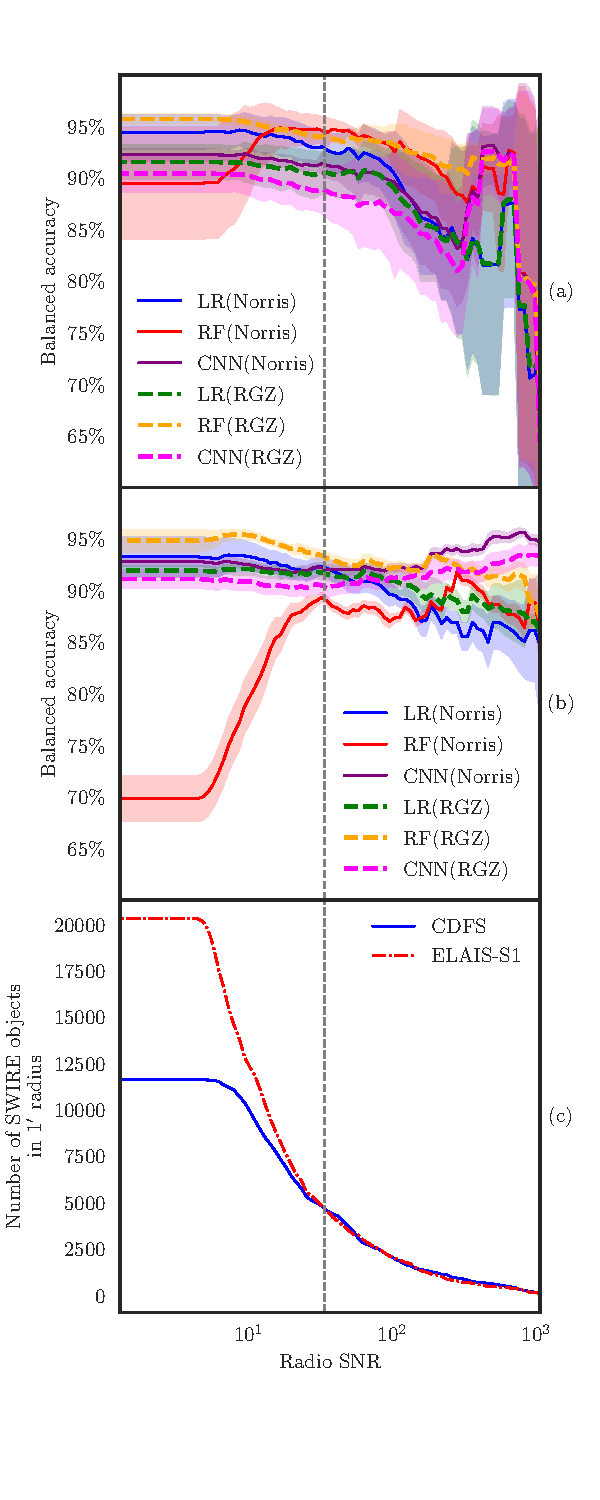
\includegraphics[width=\columnwidth, clip,
                     trim={0 2cm 0 1cm}]{images/accuracies-flux-snr.pdf}
    \caption{(a) Balanced accuracies of classifiers trained and tested on CDFS
      with different signal-to-noise ratio (SNR) cutoffs for the test set. A
      SWIRE object is included in the test set if it is within $1'$ of a radio
      component with greater SNR than the cutoff. Different coloured lines
      indicate different classifier/training labels combinations, where LR is
      logistic regression, RF is random forests, CNN is convolutional neural
      networks, and Norris and RGZ are the expert and Radio Galaxy Zoo label
      sets respectively. Filled areas represent standard deviations across
      CDFS quadrants. (b) Balanced accuracies of classifiers trained on CDFS
      and tested on ELAIS-S1. (c) A cumulative distribution plot of SWIRE
      objects associated with a radio object with greater SNR than the cutoff.
      The grey dashed line shows the SNR level at which the number of SWIRE
      objects above the cutoff is equal for CDFS and ELAIS-S1. This SNR level
      is approximately $0.02$.}
    \label{fig:accuracies-flux}
  \end{figure}

\section{Discussion}

  Our main result is that it is possible to cast radio host galaxy
  cross-identification as a machine learning task for which standard methods
  can be applied. These methods can then be trained with a variety of label
  sets derived from cross-identification catalogues. While we have not outperformed baseline methods, we have demonstrated that for a very accurate binary classifier, good cross-identification results can be obtained using our method. Future work could even combine multiple catalogues or physical priors to boost performance.

  Nearest neighbours approachs outperform most methods we investigated, notably including Radio Galaxy Zoo. This is likely due to the large number of compact or partially-resolved objects in ATLAS. This result shows that for compact
  objects, methods that do not use machine learning such as a
  nearest-neighbours approach or likelihood ratio (Weston et al. in prep) should be
  preferred to machine learning methods.

  The accuracies of our trained cross-identification methods generally fall
  far below the best possible accuracy attainable using our approach, indicated
  by the green lines in Figures \ref{fig:cross-id-accuracy} and
  \ref{fig:elais-cross-id-accuracy}. The balanced accuracies attained by our
  binary classifiers indicate that there is significant room for improvement
  in classification. The classification accuracy can be improved by better
  model selection and more training data, particularly for convolutional
  neural networks. There is a huge variety of ways to build a convolutional
  neural network, and we have only investigated one architecture. For an
  exploration of different convolutional neural network architectures
  applied to radio astronomy, see Lukic et al. (in prep). Convolutional
  neural networks generally require more training data than other machine
  learning models and we have only trained our networks on a few hundred
  sources. We would thus expect performance on the classification task to
  greatly increase with larger training sets.

  Another problem is that of the window size used to select radio features.
  Increasing window size would increase computational expense, but provide
  more information to the models. Results are also highly sensitive to how
  large the window size is compared to the size of the radio galaxy we are
  trying to cross-identify, with large angular sizes requiring large window
  sizes to ensure that the features contain all the information needed to
  localise the host galaxy. An ideal implementation of our method would most
  likely represent a galaxy using radio images taken at multiple window
  sizes, but this is considerably more expensive.

  Larger training sets, better model selection, and larger window sizes
  would improve performance, but only so far: we would still be bounded
  above by the estimated ``perfect'' classifier accuracy. From this point,
  the performance can only be improved by improving upon our broken
  assumptions. We detailed these assumptions in \autoref{sec:limitations},
  and we will discuss here how these could be resolved. Our assumption that the host galaxy is contained within the search radius could be improved by
  dynamically choosing the search radius, perhaps based on the angular
  extent of the galaxy, or the redshift of candidate hosts. Radio morphology information may allow us to select relevant radio data and hence relax the assumption that a $1'$-wide radio image represents just one, whole radio source. Finally, our
  assumption that the host galaxy is visible in infrared is technically not
  needed, as the sliding window approach we have employed will still work
  even if there are no visible host galaxies --- instead of classifying
  candidate hosts, simply classify each pixel in the radio image. The
  downside of removing candidate hosts is that we are no longer able to
  reliably incorporate host galaxy information such as colour and redshift,
  though this could be resolved by treating pixels as potentially invisible
  candidate hosts with noisy features.

  We observe that Radio Galaxy Zoo-trained methods perform comparably to
  methods trained on expert labels. This shows that the crowdsourced labels
  from Radio Galaxy Zoo will indeed provide a valuable source of training
  data for future machine learning methods in radio astronomy.

  \autoref{fig:accuracies-flux} reveals interesting behaviour of different
  classifier models at different flux cutoffs. Logistic regression and
  convolutional neural networks seem relatively independent of flux, with
  these models performing well on the fainter ELAIS-S1 sources even when
  they were trained on the generally brighter objects in CDFS. Conversely,
  random forests were sensitive to the changes in flux distribution between
  datasets. This shows that not all models behave similarly on radio data,
  and it is therefore important to investigate multiple models when
  developing machine learning methods for radio astronomy.

  Our methods can be easily incorporated into other cross-identification
  methods or used as an extra data source for source identification. This is
  because we have essentially produced a scoring function, which rates
  galaxies based on the probability that they are a host galaxy. For
  example, our method could be used to disambiguate between candidate host
  galaxies selected by model-based algorithms, or used to weight candidate
  host galaxies while a source identifier attempts to associate radio
  components. Our method can also be extended using other data sources; for
  example, information from source identification algorithms could be
  incorporated into the feature set of candidate host galaxies.

\section{Summary}

  We present a machine learning approach for cross-identification of radio
  components with their corresponding infrared host galaxy. We trained our
  methods on expert and crowdsourced cross-identification catalogues, and
  applied these methods on the CDFS and ELAIS-S1 fields of ATLAS. The Radio
  Galaxy Zoo-trained models performed comparably to the expert-trained models
  on the cross-identification task, showing that crowdsourced labels are
  useful for training machine learning methods for cross-identification. While
  our cross-identification performance is not as high as would be ideal, we
  make no assumptions on the binary classification model used in our methods
  and so we expect the performance to be improved by further experimentation
  and model selection. Our method provides a useful framework for generalising
  cross-identification catalogues to unseen areas of the sky and can be
  incorporated into existing methods.

\section{Acknowledgements}

  This publication has been made possible by the participation of more than
  11~000 volunteers in the Radio Galaxy Zoo project. Their contributions are
  individually acknowledged at \url{http://rgzauthors.galaxyzoo.org}. Parts of
  this research were conducted by the Australian Research Council Centre of
  Excellence for All-sky Astrophysics (CAASTRO), through project number
  CE110001020. Radio Galaxy Zoo makes use of data products from the Wide-field
  Infrared Survey Explorer and the Very Large Array. The Wide-field Infrared
  Survey Explorer is a joint project of the University of California, Los
  Angeles, and the Jet Propulsion Laboratory/California Institute of
  Technology, funded by the National Aeronautics and Space Administration. The
  National Radio Astronomy Observatory is a facility of the National Science
  Foundation operated under cooperative agreement by Associated Universities,
  Inc. This research has made use of the NASA/IPAC Extragalactic Database
  (NED) which is operated by the Jet Propulsion Laboratory, California
  Institute of Technology, under contract with the National Aeronautics and
  Space Administration. The figures in this work made use of Astropy, a
  community-developed core Python package for Astronomy \citep{astropy}.
  Partial support for L.~Rudnick was provided by U.S. National Science
  Foundation grants AST1211595 and 1714205 to the University of Minnesota. The
  Australia Telescope Compact Array is part of the Australia Telescope, which
  is funded by the Commonwealth of Australia for operation as a National
  Facility managed by CSIRO. We also acknowledge H.~Andernach, A.~Tran, and C.~Wolf for their contributions to this paper.

%
%%%%%%%%%%%%%%%%%%%% REFERENCES %%%%%%%%%%%%%%%%%%
\bibliographystyle{mnras}
\bibliography{rgz-cdfs-ms}

%%%%%%%%%%%%%%%%%%%%%%%%%%%%%%%%%%%%%%%%%%%%%%%%%%
% \clearpage
% \appendix
% \section{Tables of accuracies}

% In \autoref{tab:average-accuracies} and \autoref{tab:average-accuracies-elais}
% we list the balanced accuracies of classifiers on CDFS and ELAIS-S1
% respectively, averaged over quadrants. In \autoref{tab:cross-id-accuracies}
% and \autoref{tab:cross-id-accuracies-elais} we list the accuracies of our
% method on the cross-identification task on CDFS and ELAIS-S1 respectively,
% averaged over quadrants.

% \begin{table*}
%   \caption{Average balanced accuracies across quadrants shown in
%     \autoref{fig:ba} for CDFS. Uncertainties represent standard
%     deviations. The classifiers were trained and tested on compact
%     sources, resolved sources, and all sources separately. `Labeller'
%     indicates what label set the classifiers were trained on. `Norris' is
%     the expert label set, `RGZ' is the Radio Galaxy Zoo label set.%, and
%     `LR' refers to logistic regression, `CNN' refers to our convolutional
%     neural network, and `RF' refers to random forests. `Labels' refers to a
%     classifier that simply reads the test labels, and hence represents the
%     balanced accuracy of the Radio Galaxy Zoo citizen scientists.}
%   \label{tab:average-accuracies}
%   \begin{tabular}{llccc}
%     \hline
%     Labeller & Classifier & Mean `Compact' accuracy & Mean `Resolved' accuracy & Mean `All' accuracy\\
%      & & (per cent) & (per cent) & (per cent)\\
%     \hline
%     Norris & CNN & $92.6 \pm 0.7$ & $91.2 \pm 0.5$ & $92.1 \pm 0.6$\\
%      & LR & $91.6 \pm 1.0$ & $93.2 \pm 1.0$ & $93.1 \pm 1.2$\\
%      & RF & $97.5 \pm 0.6$ & $90.9 \pm 4.8$ & $96.7 \pm 2.3$\\
%      \\
%     RGZ & CNN & $87.8 \pm 0.7$ & $89.2 \pm 0.7$ & $87.7 \pm 0.9$\\
%      & LR & $91.4 \pm 0.8$ & $89.8 \pm 0.8$ & $90.8 \pm 1.4$\\
%      & RF & $94.0 \pm 0.6$ & $94.7 \pm 0.6$ & $94.1 \pm 0.3$\\
%      & Labels & $94.5 \pm 0.8$ & $89.0 \pm 2.5$ & $93.1 \pm 0.9$\\
%     \hline
%   \end{tabular}
% \end{table*}

% \begin{table}
%   \caption{Average cross-identification accuracies across quadrants.
%     Uncertainties represent standard deviations across quadrants and, for
%     the `random' classifier, 25 random classifiers. Columns and
%     classifiers as defined in \autoref{tab:average-accuracies}.  A
%     `perfect' classifier reads the expert labels directly and hence
%     represents the maximum attainable accuracy on the test set under our
%     assumptions. A `random' classifier generates uniform random class
%     probabilities and hence represents the expected minimum attainable
%     accuracy with our cross-identification method.}
%     \label{tab:cross-id-accuracies}
%   \begin{tabular}{llcc}
%     \hline
%     Labeller & Classifier & Mean `Resolved' & Mean `All'\\
%     && accuracy (per cent) & accuracy (per cent)\\
%     \hline
%       NN & --- & $75.7 \pm 7.9$ & $93.4 \pm 0.8$\\
%       Random & --- & $22.3 \pm 9.2$ & $83.2 \pm 4.7$\\
%       Norris & CNN & $74.3 \pm 12.3$ & $94.8 \pm 1.1$\\
%        & LR & $76.0 \pm 3.2$ & $94.0 \pm 1.6$\\
%        & RF & $81.3 \pm 3.7$ & $94.4 \pm 2.0$\\
%        & Perfect & $99.0 \pm 1.8$ & $98.1 \pm 1.7$\\
%       RGZ & CNN & $68.1 \pm 9.2$ & $92.2 \pm 0.8$\\
%        & LR & $74.5 \pm 5.1$ & $94.2 \pm 1.3$\\
%        & RF & $69.6 \pm 10.5$ & $94.1 \pm 2.2$\\
%        & Labels & $56.7 \pm 5.9$ & $90.5 \pm 2.6$\\
%     \hline
%   \end{tabular}
% \end{table}

% \begin{table*}
%   \caption{Average balanced accuracies across quadrants shown in
%     \autoref{fig:elais-ba} for ELAIS-S1. Uncertainties represent standard
%     deviations. The classifiers were applied to compact sources, resolved
%     sources, and all sources separately.}
%   \label{tab:average-accuracies-elais}
%   \begin{tabular}{ccccc}
%     \hline
%     Labeller & Classifier & Mean `Compact' accuracy & Mean `Resolved' accuracy & Mean `All' accuracy \\
%      & & (per cent) & (per cent) & (per cent)\\
%     \hline
%     Norris & CNN & $94.8 \pm 0.2$ & $92.8 \pm 0.5$ & $94.4 \pm 0.2$ \\
%      & LR & $94.6 \pm 0.4$ & $93.3 \pm 2.0$ & $95.3 \pm 0.1$ \\
%      & RF & $87.4 \pm 5.6$ & $71.5 \pm 2.3$ & $86.0 \pm 2.6$ \\
%      \\
%     RGZ & CNN & $88.8 \pm 0.6$ & $89.9 \pm 0.3$ & $88.5 \pm 0.3$ \\
%      & LR & $93.2 \pm 0.5$ & $91.4 \pm 0.3$ & $91.6 \pm 0.6$ \\
%      & RF & $94.9 \pm 0.2$ & $95.2 \pm 0.3$ & $95.1 \pm 0.2$ \\
%      \hline
%   \end{tabular}
% \end{table*}

% \begin{table}
%   \caption{Average cross-identification accuracies for ELAIS-S1.
%     Uncertainties represent standard deviations across classifiers trained
%     on CDFS quadrants. Columns and classifiers as defined in Table
%     \ref{tab:average-accuracies}.  A `perfect' classifier reads the expert
%     labels directly and hence represents the maximum attainable accuracy
%     under our assumptions. A `random' classifier generates uniform random
%     class probabilities and hence represents the expected minimum attainable
%     accuracy with our cross-identification method.}
%     \label{tab:cross-id-accuracies-elais}
%   \begin{tabular}{llcc}
%     \hline
%     Labeller & Classifier & Mean `Resolved' & Mean `All'\\
%     && accuracy (per cent) & accuracy (per cent)\\
%     \hline
%     NN & --- & $92.8 \pm 0.0$ & $95.5 \pm 0.0$\\
%     Random & --- & $26.6 \pm 2.1$ & $61.9 \pm 1.1$\\
%     Norris & CNN & $89.4 \pm 1.4$ & $95.1 \pm 0.3$\\
%      & LR & $89.7 \pm 1.8$ & $96.0 \pm 0.3$\\
%      & RF & $81.0 \pm 4.7$ & $94.7 \pm 0.7$\\
%      & Perfect & $99.8 \pm 0.0$ & $99.6 \pm 0.0$\\
%     RGZ & CNN & $84.6 \pm 0.6$ & $90.4 \pm 0.4$\\
%      & LR & $92.7 \pm 0.2$ & $95.8 \pm 0.3$\\
%      & RF & $90.3 \pm 2.4$ & $95.7 \pm 0.9$\\
%     \hline
%   \end{tabular}
% \end{table}


% \section{Catalogues}

%   \begin{table*}
%     \caption{Predicted probabilities that each object in SWIRE is a host
%       galaxy. Probabilities are reported for each predictor. $C(A\ /\ B)$
%       indicates the predictor using classifier model $C$, trained on label set
%       $A$ on data set $B$. Ellipsis indicates columns that have been omitted.
%       The omitted columns are all other combinations of classifier, label set,
%       and data set. If a SWIRE object does not appear in the table, then it
%       was further than 1 arcmin from an ATLAS object and hence has a predicted
%       probability of zero by our assumptions. Full table electronic.}
%     \label{tab:probs}
%     \begin{tabular}{ccccccccccccccccccccc}
%       \hline
%       SWIRE & RA & Dec & CNN(Norris / All) & & RF(RGZ / Resolved) \\\hline
%       SWIRE3\textunderscore{}J032559.15-284724.2 & 51.4965 & -28.7901 & 0.0001 & $\cdots$ & 0.1170 \\
%       SWIRE3\textunderscore{}J032559.91-284728.9 & 51.4996 & -28.7914 & 0.0004 & $\cdots$ & 0.0000 \\
%       SWIRE3\textunderscore{}J032600.02-284736.9 & 51.5001 & -28.7936 & 0.0002 & $\cdots$ & 0.0451 \\
%       SWIRE3\textunderscore{}J032600.13-284637.5 & 51.5005 & -28.7771 & 0.0004 & $\cdots$ & 0.0637 \\
%       SWIRE3\textunderscore{}J032600.13-284715.7 & 51.5006 & -28.7877 & 0.0014 & $\cdots$ & 0.0153 \\
%       SWIRE3\textunderscore{}J032600.98-284705.4 & 51.5041 & -28.7848 & 0.0205 & $\cdots$ & 0.0000 \\
%       SWIRE3\textunderscore{}J032601.03-284711.6 & 51.5043 & -28.7866 & 0.0699 & $\cdots$ & 0.0000 \\
%       SWIRE3\textunderscore{}J032601.56-284131.0 & 51.5065 & -28.692 & 0.0001 & $\cdots$ & 0.0000 \\
%       SWIRE3\textunderscore{}J032601.60-284207.5 & 51.5067 & -28.7021 & 0.0000 & $\cdots$ & 0.0000 \\\hline
%     \end{tabular}
%   \end{table*}

%  \begin{table*}
%     \small
%     \caption{Predicted host galaxy cross-identifications for each object in
%       ATLAS. Cross-identifications are reported for each predictor, with the
%       predictor listed as in \autoref{tab:probs}. The cross-identification
%       given by \citet{norris06} for CDFS or \citet{middelberg08} for ELAIS-S1
%       is included in the `Expert' column. For CDFS, the cross-identification
%       given by the Radio Galaxy Zoo consensus is included in the `RGZ' column,
%       along with the corresponding consensus levels for the radio morphology
%       and host cross-identification tasks (see Wong et al., in prep, for
%       details on how consensus is calculated). Low radio consensus indicates
%       that the component has multiple nearby components (and thus is more
%       impacted by our assumption that the source is isolated), and low
%       infrared consensus indicates that the host galaxy is unclear in the
%       SWIRE image (possibly due to multiple nearby candidate host galaxies).
%       Full table electronic.}
%     \begin{tabular}{ccccc}
%       \hline
%       ATLAS & RA & Dec & Expert & RGZ \\\hline
%       ATLAS3\textunderscore{}J032602.82-284708.1C & 51.511734 & -28.785575 & SWIRE3\textunderscore{}J032603.15-284708.5 & -\\
%       ATLAS3\textunderscore{}J032615.49-284629.4C & 51.564555 & -28.774847 & SWIRE3\textunderscore{}J032615.41-284630.7 & SWIRE3\textunderscore{}J032615.41-284630.7\\
%       ATLAS3\textunderscore{}J032615.55-280559.8C & 51.564799 & -28.099955 & SWIRE3\textunderscore{}J032615.52-280559.8 & SWIRE3\textunderscore{}J032615.52-280559.8\\
%       ATLAS3\textunderscore{}J032617.35-280710.2C & 51.572279 & -28.119491 & SWIRE3\textunderscore{}J032617.89-280707.2 & SWIRE3\textunderscore{}J032617.89-280707.2\\
%       ATLAS3\textunderscore{}J032625.13-280909.8C & 51.604711 & -28.152731 & SWIRE3\textunderscore{}J032625.19-280910.1 & SWIRE3\textunderscore{}J032625.19-280910.1\\
%       ATLAS3\textunderscore{}J032629.10-280650.1C & 51.621251 & -28.113924 & SWIRE3\textunderscore{}J032629.13-280650.7 & SWIRE3\textunderscore{}J032626.74-280636.7\\
%       ATLAS3\textunderscore{}J032629.61-284052.7C & 51.623385 & -28.681315 & SWIRE3\textunderscore{}J032629.54-284055.8 & SWIRE3\textunderscore{}J032629.54-284055.8\\
%       ATLAS3\textunderscore{}J032629.92-284753.5C & 51.624653 & -28.798195 & SWIRE3\textunderscore{}J032629.81-284754.4 & SWIRE3\textunderscore{}J032629.81-284754.4\\
%       ATLAS3\textunderscore{}J032630.66-283657.3C & 51.62777 & -28.615917 & SWIRE3\textunderscore{}J032630.64-283658.0 & SWIRE3\textunderscore{}J032628.56-283744.8\\
%       \hline
%     \end{tabular}
%     \begin{tabular}{ccccccccccccccccccccccccc}
%       \hline
%       RGZ radio consensus & RGZ IR consensus & CNN(Norris / All) & & RF(RGZ / Resolved) \\\hline
%       0.4516 & 0.3214 & SWIRE3\textunderscore{}J032602.36-284711.5 & $\cdots$ & SWIRE3\textunderscore{}J032603.60-284627.4 \\
%       0.2941 & 0.8000 & SWIRE3\textunderscore{}J032615.41-284630.7 & $\cdots$ & SWIRE3\textunderscore{}J032615.41-284630.7 \\
%       0.5625 & 0.8333 & SWIRE3\textunderscore{}J032615.52-280559.8 & $\cdots$ & SWIRE3\textunderscore{}J032615.52-280559.8 \\
%       0.4146 & 1.0000 & SWIRE3\textunderscore{}J032617.89-280707.2 & $\cdots$ & SWIRE3\textunderscore{}J032617.89-280707.2 \\
%       0.3158 & 0.6667 & SWIRE3\textunderscore{}J032625.19-280910.1 & $\cdots$ & SWIRE3\textunderscore{}J032625.19-280910.1 \\
%       0.3333 & 1.0000 & SWIRE3\textunderscore{}J032629.13-280650.7 & $\cdots$ & SWIRE3\textunderscore{}J032629.13-280650.7 \\
%       0.2676 & 1.0000 & SWIRE3\textunderscore{}J032629.54-284051.9 & $\cdots$ & SWIRE3\textunderscore{}J032629.54-284051.9 \\
%       1.0000 & 0.8571 & SWIRE3\textunderscore{}J032629.81-284754.4 & $\cdots$ & SWIRE3\textunderscore{}J032629.81-284754.4 \\
%       0.3611 & 0.7308 & SWIRE3\textunderscore{}J032630.64-283658.0 & $\cdots$ & SWIRE3\textunderscore{}J032628.56-283744.8 \\
%       \hline
%     \end{tabular}
%     \label{tab:cids}
%   \end{table*}

%   The predicted probabilities for each SWIRE object are listed in \autoref{tab:probs}. A full version of the table is available electronically.  The columns are defined as follows:
%   \begin{itemize}
%     \item {\em Column 1}  -- SWIRE. The SWIRE object name given in \citet{surace05swire}.
%     \item {\em Column 2} -- RA. The right ascension of the SWIRE object in decimal degrees (J2000).
%     \item {\em Column 3} -- Dec. The declination of the SWIRE object in decimal degrees (J2000).
%     \item {\em Columns 4 -- 21} -- $C(A\ /\ B)$. The predicted probability
%       that the SWIRE object is a host galaxy according to classifier $C$ trained
%       on subset $B$ of label set $A$. `LR' indicates logistic regression, `RF'
%       indicates random forests, `CNN' indicates convolutional neural networks,
%       `Norris' indicates the expert labels, and `RGZ' indicates the Radio Galaxy
%       Zoo labels.
%   \end{itemize}

%   The predicted cross-identifications for each ATLAS object are listed in
%   \autoref{tab:cids}. A full version of the table is available electronically.
%   The columns are defined as follows:
%   \begin{itemize}
%     \item {\em Column 1}  -- ATLAS. The ATLAS object name given in \citet{franzen15}.
%     \item {\em Column 2} -- RA. The right ascension of the ATLAS object in decimal degrees (J2000).
%     \item {\em Column 3} -- Dec. The declination of the ATLAS object in decimal degrees (J2000).
%     \item {\em Column 4} -- Expert. The expert SWIRE cross-identification.
%       This is the SWIRE object associated with the ATLAS object according to
%       either \citet{norris06} or \citet{middelberg08} for CDFS and ELAIS-S1,
%       respectively.
%     \item {\em Column 5} -- RGZ. The Radio Galaxy Zoo cross-identification.
%       This is the SWIRE object associated with the ATLAS object according to
%       Radio Galaxy Zoo.
%     \item {\em Column 5} -- RGZ radio consensus. The percentage agreement on
%       the radio source according to Radio Galaxy Zoo. Lower numbers tend to
%       indicate more complex sources. For more information on how consensus is
%       generated, see Wong et al. (in prep).
%     \item {\em Column 6} -- RGZ IR consensus. The percentage agreement on
%       the host galaxy cross-identification according to Radio Galaxy Zoo.
%       Lower numbers tend to indicate sources that are harder to
%       cross-identify. For more information on how consensus is generated, see Wong et al. (in prep).
%     \item {\em Columns 7 -- 25} -- $C(A\ /\ B)$. The predicted
%       cross-identification according to classifier $C$ trained on subset $B$
%       of label set $A$. `LR' indicates logistic regression, `RF' indicates
%       random forests, `CNN' indicates convolutional neural networks, `Norris'
%       indicates the expert labels, and `RGZ' indicates the Radio Galaxy Zoo
%       labels.
%   \end{itemize}

% Don't change these lines
\bsp	% typesetting comment
\label{lastpage}
\end{document}
